\documentclass[12pt,a4paper]{article}
%\usepackage{algorithmic}
\usepackage[utf8]{inputenc}
\usepackage[brazil]{babel}
\usepackage{graphicx}
\usepackage[linktocpage]{hyperref}
\usepackage{abnt-alf}
\usepackage[top=3cm,bottom=2cm,left=3cm,right=2cm]{geometry}
\usepackage{indentfirst}
\usepackage{longtable}
\usepackage{lscape}
\usepackage{amsmath}
\usepackage{amsfonts}
\usepackage{float}
\usepackage{chngcntr}
\usepackage{lscape}
\usepackage[section]{algorithm}
\usepackage{savesym}
\usepackage{vaucanson-g}
\savesymbol{State}
\usepackage{algcompatible}
\let\vState=\origState
\usepackage{rotating}

\floatname{algorithm}{Algoritmo}

\newenvironment{definition}[1][Definição]{\begin{trivlist}
\item[\hskip \labelsep {\bfseries #1}]}{\end{trivlist}}

\counterwithin{equation}{section}
\counterwithin{figure}{section}
\counterwithin{table}{section}

\algrenewcommand\algorithmicindent{0.9em}%

\newtheorem{theorem}{Teorema}[section]
\newtheorem{lemma}[theorem]{Lema}
\newtheorem{proposition}[theorem]{Proposição}
\newtheorem{corollary}[theorem]{Corolário}

\newenvironment{proof}[1][Prova]{\begin{trivlist}
\item[\hskip \labelsep {\bfseries #1}]}{\end{trivlist}}

% CAPA
\pagestyle{empty}
\begin{document}
\begin{center}
\large  \textbf{UNIVERSIDADE PRESBITERIANA MACKENZIE}
\large  \textbf{PROGRAMA DE PÓS-GRADUAÇÃO EM}\\
\large  \textbf{ENGENHARIA ELÉTRICA}\\
\vskip 2.0cm
\textbf{\large Wander Lairson Costa}\\
\vskip 3.5cm
\setlength{\baselineskip}{1.5\baselineskip}
\textbf{\large Avanços no estudo de complexidade em linguagem regular de
autômatos celulares elementares}\\
\vskip 4.0cm
\end{center}
\hfill{\vbox{\hsize=8.5cm\noindent\strut
Dissertação de Mestrado apresentada ao\break
Programa de Pós-Graduação em Engenharia\break
Elétrica, como parte das Exigências para\break
Obtenção do Grau de Mestre em Engenharia\break
Elétrica, na Área de Concentração em\break
Engenharia da Computação.}\\
\strut}
\vskip 2.0cm
\textbf{\normalsize Orientador: Pedro Paulo Balbi de Oliveira}\\
\vskip 2.0cm
\begin{center}
São Paulo\\
2012\\
\end{center}

% AGRADECIMENTOS
\newpage
\thispagestyle{plain}
\pagenumbering{roman}
\begin{center}
\large  
\textbf{AGRADECIMENTOS}
\end{center}
\renewcommand{\baselinestretch}{0.6666666}

Agradeço primeiramente a Deus, por guiar meus passos e a meus pais, que me
ensinaram que a fé realmente move montanhas e por terem-me mostrado o
verdadeiro significado da palavra caráter.

Agradeço também aos colegas de curso, que sempre me incentivaram, em especial
agradeço aos meus amigos Israel Florentino dos Santos e Adílson Eduardo
Spagiari.

Por fim, mas não menos importante, agradeço ao meu orientador e amigo 
Prof. Pedro Paulo Balbi de Oliveira, pelo trabalho de orientação com
dedicação, empenho e amizade, e que tanto contribuiu para a elaboração e
evolução deste estudo.
\\[0.5cm]

% RESUMO
\newpage
\thispagestyle{plain}
%\pagenumbering{roman}
\begin{center}
\large  
\textbf{RESUMO}
\end{center}
\renewcommand{\baselinestretch}{0.6666666}
Autômatos celulares (ACs) são sistemas totalmente discretos que agem
localmente de forma simples e determinística, mas cujo comportamento
global resultante pode ser extremamente complexo. O conjunto de possíveis
configurações globais em um passo de tempo $t$ finito para um AC pode ser
descrito por uma linguagem regular, a qual por sua vez pode ser representada
por meio de um autômato finito (AF). Uma classe de AFs relevante para este
trabalho são os chamados grafos de processo, que são AFs em que todos os
estados são iniciais e finais, pois estes permitem uma notação matricial
compacta e inequívoca. Estuda-se aqui a complexidade da evolução temporal
dos ACs, onde trabalhos anteriores são revisados e discutidos, apontando
problemas nos experimentos e seu impacto nos resultados. Também inicia-se
uma nova abordagem para o problema, substituindo a representação dos
grafos de processo que descrevem a configuração a cada passo de tempo
por matrizes de adjacência deles derivadas. De fato, estende-se a notação
clássica de matriz de adjacência, já que ela se mostra insuficiente para
descrever completamente os grafos de processo em questão. Com essa nova
notação, mostra-se que é possível obter o algoritmo que gere o grafo de
processo de tempo $t$ para cada uma das regras estudadas. Conclui-se que,
embora houve avanços para o problema do grafo limite, este ainda permanece
aberto, e sugestões para continuação da pesquisa são dadas.
\\[0.5cm]
\begin{flushleft}
{\bf Palavras-chave:} {\it Autômato celular elementar, comportamento limite,
linguagem regular, matriz de adjacência, complexidade, autômato finito.}
\end{flushleft}

% SUMÁRIO
\newpage
\thispagestyle{empty}
\tableofcontents

% DESENVOLVIMENTO
\newpage
\pagestyle{plain}
\pagenumbering{arabic}
\renewcommand{\baselinestretch}{1.5} 
\normalsize

\newcommand{\citecustom}[1]{[\citeauthoronline{#1}, \citeyear{#1}]}

\section{Introdução}

Autômatos celulares (ACs) são sistemas discretos que apresentam um comportamento
local extremamente simples, mas cujo comportamento global pode ser tão
complexo quanto uma máquina de Turing \citecustom{wolfram1984a}. Ele
é caracterizado por um reticulado de células cujos estados posteriores
dependem dos estados anteriores de si próprias e de suas vizinhas.
Este tipo de comportamento, que é localmente simples mas globalmente
complexo dá origem à chamada \textit{computação emergente}, e é
a base da utilização dos ACs na modelagem de diversos sistemas naturais.

A vizinhança das células de um AC pode ser definida por
um \textit{raio} centrado na célula em questão, de forma a englobar
todas as células dentro do raio. Um AC
elementar possui raio igual a 1 e conjunto de estados $\{0,1\}$, o que
permite a definição de um espaço de 256 regras possíveis, que são
usualmente identificadas por um número entre 0 e 255 \citecustom{wolfram1984}.
Este trabalho estuda um subconjunto dos ACs elementares, que consiste
em 26 regras estudadas em \citecustom{trafaniuc2004} e 
\citecustom{miki2006}.

O comportamento limite de ACs pode ser descrito por meio
de linguagens formais, a partir das cadeias ou
palavras formadas por seu alfabeto \citecustom{lewis2008}.
A classe mais simples de linguagens formais é
a das linguagens regulares, que pode ser gerada por uma gramática regular ou
pelas chamadas expressões regulares. Qualquer linguagem regular pode ser
reconhecida por um autômato finito (AF), que é uma modalidade de autômato que
possui memória restrita. As linguagens regulares são o tipo mais simples
de linguagem na hierarquia de Chomsky.

O conjunto de todas as configurações globais de um AC
elementar em um dado momento no tempo discreto pode ser descrito por
uma linguagem regular e, consequentemente, um AF
\citecustom{wolfram1984}. \citeonline{trafaniuc2004} e \citeonline{miki2006}
estudaram, em seus respectivos trabalhos, a complexidade de ACs
elementares por meio da análise da evolução dos sucessivos
AFs para diferentes instantes de tempo. Este trabalho
tem o objetivo de dar prosseguimento àqueles estudos, criticando os
experimentos anteriormente realizados e introduzindo a abordagem
de representação dos AFs por meio de matrizes de adjacência.
Sobretudo, este trabalho visa estender os resultados até então obtidos
sobre a análise da complexidade de ACs por meio de grafos.

O Capítulo \ref{sec:refteo} apresenta referencial teórico sobre 
os ACs, linguagens formais e comportamento limite.

O Capítulo \ref{sec:complexity} descreve os trabalhos anteriores, aponta
os problemas encontrados nestes e discute novos resultados obtidos.

O Capítulo \ref{sec:matrix} descreve uma nova abordagem por meio de matrizes
de adjacência. A obtenção do
grafo de processo de tempo $t$ pode ser conseguida por meio de uma nova notação de 
matrizes de adjacência em relação ao respectivo grafo de processo.

O Capítulo \ref{sec:conclude} conclui o trabalho, onde são resumidos todas
as críticas a trabalhos anteriores e os resultados conseguidos nesta pesquisa.

\newpage

\section{Autômatos celulares}\label{sec:refteo}

É comum na natureza encontrar sistemas cujo comportamento global é extremamente
complexo, ainda que as partes que formam tais sistemas sejam simples. A
complexidade é gerada pelo efeito cooperativo de componentes com regras locais
simples. Muito foi descoberto sobre a natureza dos componentes em sistemas físicos
e biológicos, mas pouco é conhecido sobre os mecanismos pelos quais tais componentes
agem cooperativamente para gerar o comportamento global observado \citecustom{wolfram1984a}.

ACs podem ser vistos como uma classe de sistemas dinâmicos que atua em um reticulado
infinito cujo tempo, espaço e estado são todos discretos e os estados de cada célula
podem ser obtidos a partir de um conjunto finito de estados possíveis \citecustom{zhisong2001}. 

ACs são, fundamentalmente, as representações matemáticas mais simples
de uma classe muito maior dos chamados \textit{sistemas complexos}, termo que se refere
a qualquer sistema dinâmico que consiste de mais do que algumas poucas - tipicamente
não lineares - partes que se interagem). Assim, ACs têm se provado
serem idealizações extremamente úteis do comportamento dinâmico de muitos sistemas
complexos reais, incluindo fluídos físicos, redes neurais, sistemas dinâmicos
moleculares, economia, entre outros \citecustom{ilachinski2002}. Por causa de sua
simplicidade subjacente, ACs são máquinas
conceituais poderosas com as quais se estuda padrões generalizados de formação. Eles
já forneceram ideias cruciais sobre auto organização de reações químicas, sistemas de
difusão, crescimento de cristais, formação de padrões de conchas e fenômenos em fluxo
de tráfego veicular, para citar alguns exemplos. Em um lado mais prático, ACs
fornecem a base de algoritmos de criptografia extremamente poderosos. Existem
até mesmo algumas sérias especulações de que ACs possam fornecer
a espinha dorsal de uma física fundamental radicalmente discreta \citecustom{ilachinski2002}.

Os primeiros estudos de ACs por John von Neumann no final da década de
40 tinham como meta desenvolver sistemas computacionais auto replicantes que também fossem
computacionalmente universais. von Neumann queria investigar dispositivos sintéticos de
computação análogos ao cérebro humano no qual a memória e as unidades de processamento
não são separadas uma da outra, e que fossem massivamente paralelos e capazes de se
auto reparar e reproduzir dado o material base necessário. Segundo sugestões de
Stanislaw Ulam, von Neumann visualizou um universo discreto consistindo de uma grade
bidimensional de máquinas de estado finito, chamadas células, interconectadas
internamente umas com as outras \citecustom{kari2005}. O autômato originalmente descrito por
von Neumann é um vetor uniforme infinito bidimensional de células, onde cada célula é
conectada pelos seus quatro vizinhos ortogonais. As primeiras estruturas estudadas eram
em sua maioria de uma ou duas dimensões, apesar de dimensões maiores também terem sido
consideradas \citecustom{sarkar2000}.

Dois tópicos imediatos surgiram a partir do trabalho de von Neumann. O primeiro, em
sua maior parte na década de 60, era uma discussão sobre a construção de autômatos
auto replicantes. O segundo foi uma tentativa de capturar mais da essência de
auto replicação por meio de estudos matemáticos de propriedades detalhadas de
ACs. Durante o curso da década de 60 foram encontradas construções
mais simples de ACs capazes de auto replicação e computação
universal. No início da década de 60 foram notadas algumas características gerais
incrivelmente simples de ACs que acreditava-se serem relevantes para
auto replicação - e foram estudadas com um formalismo técnico mais elaborado. Existiram
também várias construções de ACs cujo comportamento mostraram
características particularmente simples talvez relevantes para a auto
replicação \citecustom{wolfram2002}.

A década de 80 é um período importante na história dos ACs,
largamente devido ao trabalho executado por Stephen Wolfram. A natureza de suas questões
representa uma mudança de paradigma na pesquisa com ACs. Wolfram conduziu
uma análise experimental dos padrões de crescimento de ACs
\citecustom{sarkar2000}. Seus primeiros experimentos mais importantes em ACs
datam do final de 1981. Duas características inicialmente chamaram sua atenção.
Primeiro, que iniciando de condições iniciais aleatórias, os ACs
podiam se auto organizar para produzir padrões complexos. E segundo, que em casos
como acontece com o AC elementar número 90, simples condições iniciais levavam a
padrões fractais auto similares.
Durante a metade de 1982, ele trabalhou duramente em analisar o comportamento de
ACs usando ideias da mecânica estatística, teoria de sistemas
dinâmicos e matemática discreta \citecustom{wolfram2002}.

\subsection{Autômatos celulares elementares}

Um AC unimensional consiste de uma grade bi-infinita (podendo também ter tamanho
$N$, para o caso finito), onde existe uma função de transição $\sigma: Z_r \mapsto \Sigma$,
que determina a dinâmica do AC, onde $r$ representa o raio (inteiro) de vizinhança do AC e
$\Sigma$ é o conjunto de estados possíveis de uma célula. Um AC com raio $r$ tem 
vizinhança $(-r,-r+1,\ldots,r-1,r)$, de maneira que cada vizinhança consiste
de $2r+1$ células.

Um AC \textit{elementar} é um AC unidimensional com conjunto de estados
$\Sigma = \{0,1\}$ e raio $r=1$ \citecustom{kari2005}.

Em ACs unidimensionais uma configuração inicial genérica será tipicamente atraída
para uma condição de \textit{equilíbrio} a qual é chamada de atrator \citecustom{li1987}.
Atratores representam pontos de equílibrio em sistemas dinâmicos, e, no caso de ACs,
representam configurações estáveis quando $t \mapsto \infty$. O conjunto de atratores
de um AC representa sua \textit{configuração limite}.

Embora teoricamente um autômato unidimensional possa ser interpretado como uma linha bi-infinita,
na prática existe uma quantidade fixa de células e é necessário adotar uma condição de contorno
para as células nos extremos. Um possibilidade é adotar uma condição de contorno fixa, onde
escolhe-se um determinado valor para os vizinhos não existentes das células da extrema direita
e esquerda. Outra possibilidade é adotar uma condição de contorno periódica, onde o vizinho
da direita da última célula é a primeira célula, e vice-versa, conforme ilustrado na Figura
\ref{fig:ring}.

\begin{figure}[htp]
\begin{center}
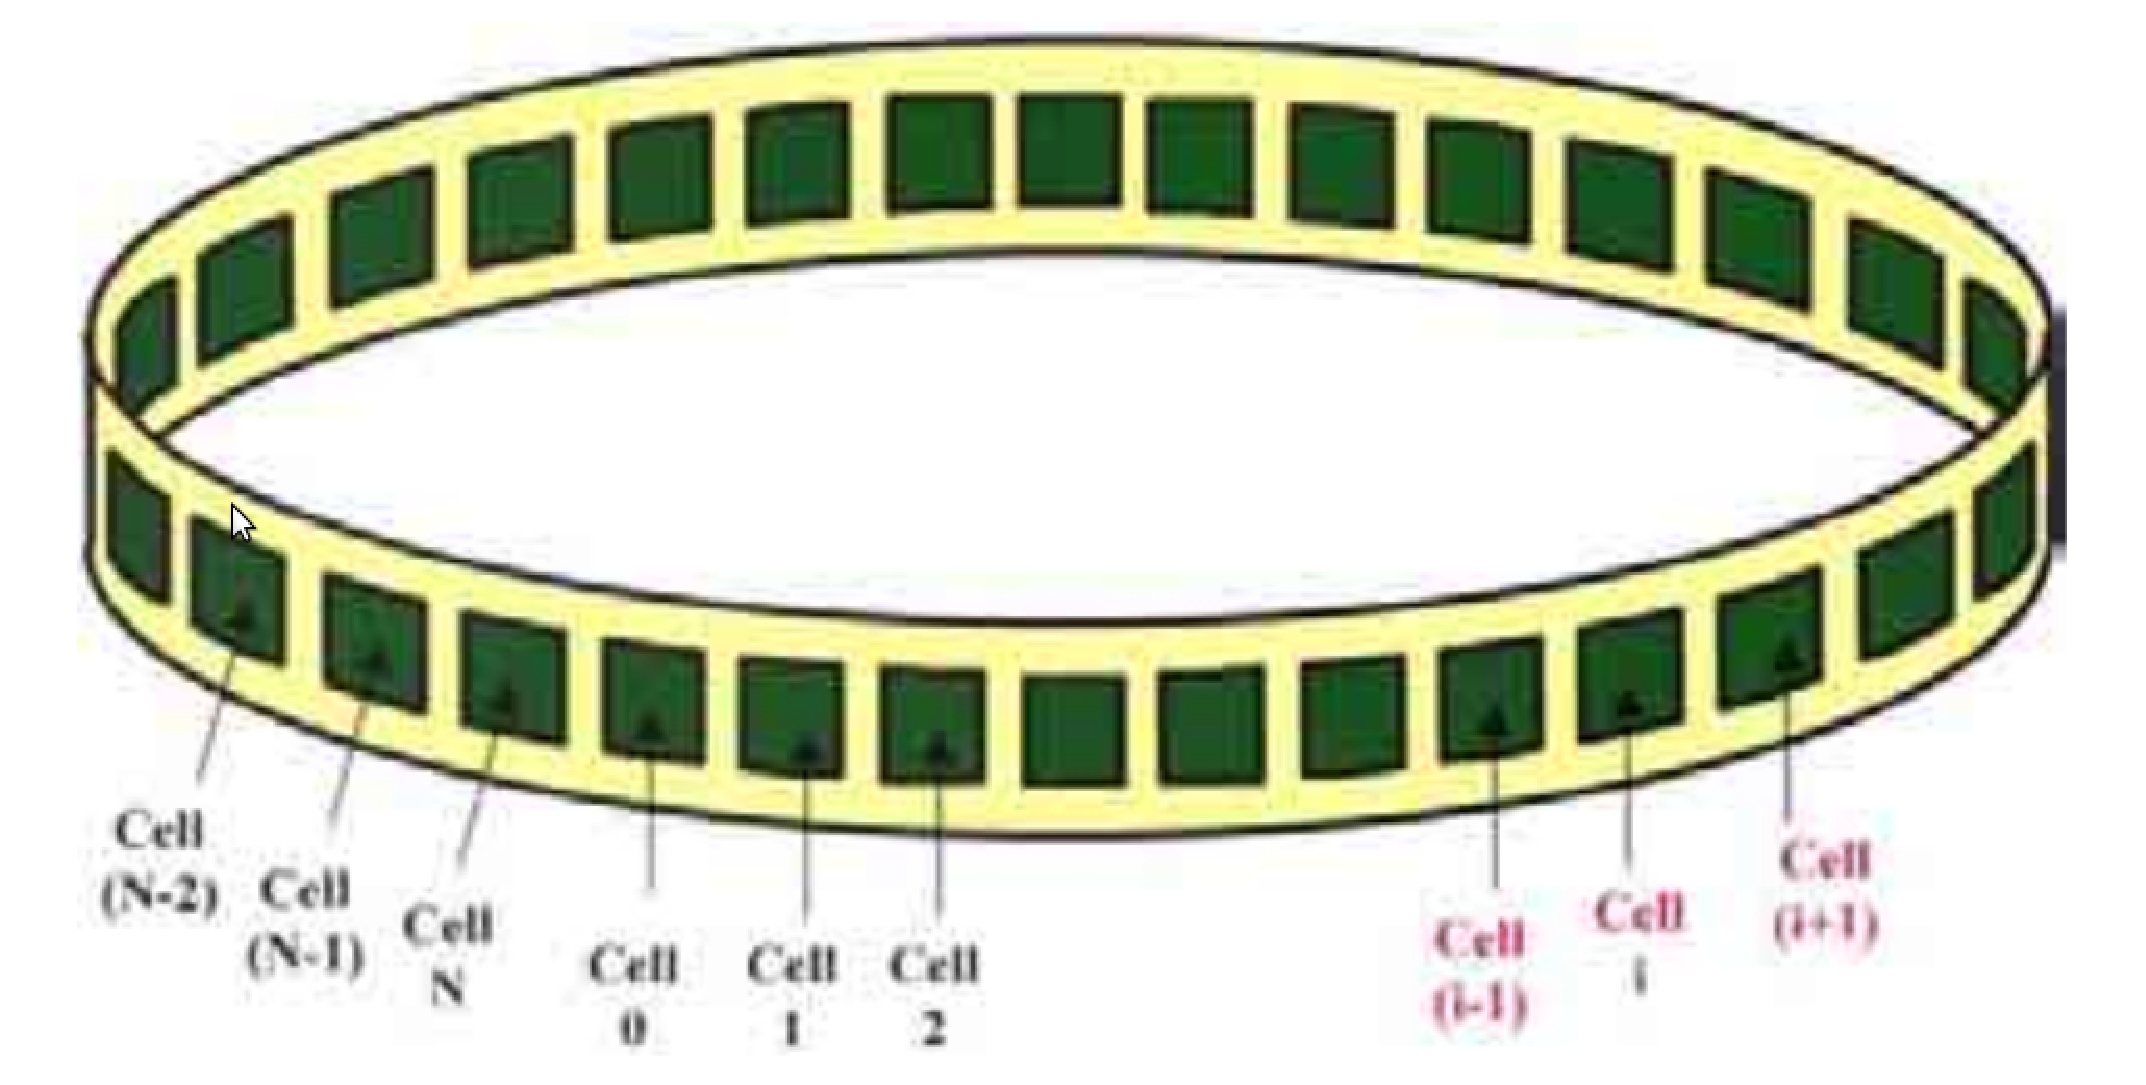
\includegraphics[scale=0.3]{img/ring.eps}
\caption{Condição de contorno periódica: a última célula é ligada à primeira,
formando um anel \citecustom{chua2002a}.}
\label{fig:ring}
\end{center}
\end{figure}

A evolução de um autômato unidimensional pode ser visualizada por meio de uma grade bidimensional
onde cada linha representa uma configuração global em um determinado instante de tempo discreto,
conforme visualizado na Figura \ref{fig:celautomaton}.

\begin{figure}[htp]
\begin{center}
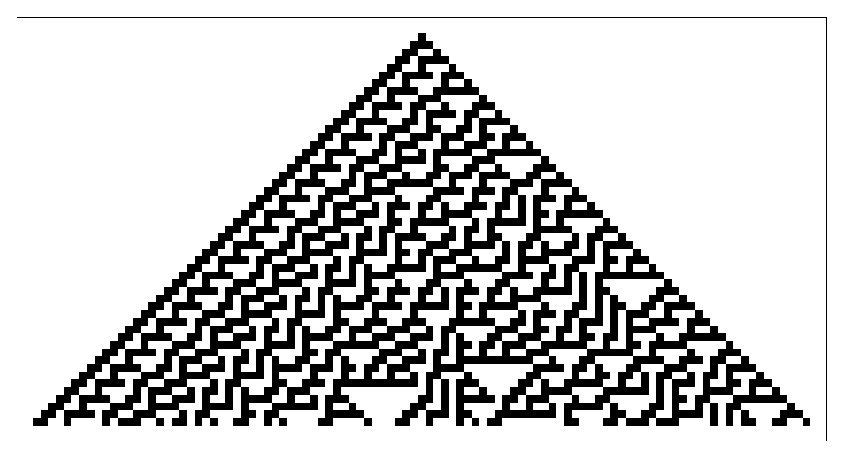
\includegraphics[scale=0.8]{img/CellularAutomaton.eps}
\caption{Evolução temporal de um autômato celular unidimensional.}
\label{fig:celautomaton}
\end{center}
\end{figure}

Existem $2^3=8$ possíveis padrões de estados dentro de uma vizinhança para ACs.
Cada combinação pode resultar nos valores 0 ou 1, assim podem existir $2^{2^3}=256$ ACs
elementares. A regra local pode ser formalizada como:

\begin{equation}
x^{t+1}_i = \phi(x^t_{i-1}, x^t_i, x^t_{i+1})
\end{equation}

\hspace{1 mm} onde $x^t_i$ é o estado da célula $i$ no instante $t$ em que a
regra local atua, e $\phi$ é a função que executa a regra local.  A Tabela
\ref{tab:localrule} mostra como é aplicada a regra local.  As regras locais
para ACs podem ser descritas por um número número binário de oito dígitos,
codificado pelo resultado das oito combinações de vizinhança da regra local
$\{x_{i-1},x_i,x_{i+1}\}$ \citecustom{wolfram1983}. No caso da Figura
\ref{fig:celnumbering}, este número é o número $90_{10}$, e este autômato
é chamado de \textit{regra 90}. Neste texto, a menos que explicitamente
dito o contrário, a referência a um AC por meio do número de sua regra se
diz respeito a um AC elementar.

\begin{table}[htp]
\begin{center}
\begin{tabular}{|c|c|c|c|}
\hline
$\mathbf{x_{i-1}}$ & $\mathbf{x_i}$ & $\mathbf{x_{i+1}}$ & $\mathbf{\phi}$ \\ \hline
1 & 1 & 1 & 0 \\ \hline
1 & 1 & 0 & 1 \\ \hline
1 & 0 & 1 & 0 \\ \hline
1 & 0 & 0 & 1 \\ \hline
0 & 1 & 1 & 1 \\ \hline
0 & 1 & 0 & 0 \\ \hline
0 & 0 & 1 & 1 \\ \hline
0 & 0 & 0 & 0 \\ \hline
\end{tabular}
\caption{Aplicação de regra local.}
\label{tab:localrule}
\end{center}
\end{table}

\begin{figure}[htp]
\begin{center}
\[ \fbox {
{\Large
\begin{tabular}{c c c c c c c c c c c}
$\frac{1 1 1}{0}$ & $\frac{1 1 0}{1}$ & $\frac{1 0 1}{0}$ & $\frac{1 0 0}{1}$ & 
$\frac{0 1 1}{1}$ & $\frac{0 1 0}{0}$ & $\frac{0 0 1}{1}$ & $\frac{0 0 0}{0}$ &
= & 90
\end{tabular}
}
} \]
\caption{Exemplo de esquema de numeração de Wolfram para ACs unidimensionais
\citecustom{wolfram1983}.}
\label{fig:celnumbering}
\end{center}
\end{figure}

\subsection{Equivalência dinâmica de regras}

Duas regras locais ${\phi}_1$ e ${\phi}_2$ são ditas equivalentes se e somente se existir
uma transformação a qual mapeia a regra ${\phi}_1$ na regra ${\phi}_2$, e vice-versa
\citecustom{chua2002a}. No caso de equivalência dinâmica, estas transformações
podem ser de três tipos:

\begin{description}

\item[Transformação de complemento (ou conjugação)] nesta transformação
todos os estados são complementados, ou seja, troca-se 0 por 1 e vice-versa,
conforme exemplificado na Figura \ref{fig:complement}.

\begin{figure}[htp]
\begin{center}
\begin{tabular}{|c|c|c|c|c|c|c|c|c|}
\hline
\textbf{Vizinhança}  & 111 & 110 & 101 & 100 & 011 & 010 & 001 & 000 \\ \hline
\textbf{$\phi$}      &  0  &  1  &  1  &  0  &  1  &  1  &  1  &  0  \\ \hline
\hline
\textbf{Complemento} & 000 & 001 & 010 & 011 & 100 & 101 & 110 & 111 \\ \hline
\textbf{$\phi$}      &  1  &  0  &  0  &  1  &  0  &  0  &  0  &  1  \\ \hline
\hline
\textbf{Reordenado}  & 111 & 110 & 101 & 100 & 011 & 010 & 001 & 000 \\ \hline
\textbf{$\phi$}      &  1  &  0  &  0  &  0  &  1  &  0  &  0  &  1  \\ \hline
\end{tabular}
\caption{Transformação de complemento.}
\label{fig:complement}
\end{center}
\end{figure}

\item[Transformação por reflexão] nesta transformação o estado do vizinho da direita é
trocado com o estado do vizinho da esquerda. A Figura \ref{fig:reflex} ilustra o processo.

\begin{figure}[htp]
\begin{center}
\begin{tabular}{|c|c|c|c|c|c|c|c|c|}
\hline
\textbf{Vizinhança}  & 111 & 110 & 101 & 100 & 011 & 010 & 001 & 000 \\ \hline
\textbf{$\phi$}      &  0  &  1  &  1  &  0  &  1  &  1  &  1  &  0  \\ \hline
\hline
\textbf{Reflexão}    & 111 & 011 & 101 & 001 & 110 & 010 & 100 & 000 \\ \hline
\textbf{$\phi$}      &  0  &  1  &  1  &  0  &  1  &  1  &  1  &  0  \\ \hline
\hline
\textbf{Reordenado}  & 111 & 110 & 101 & 100 & 011 & 010 & 001 & 000 \\ \hline
\textbf{$\phi$}      &  0  &  1  &  1  &  1  &  1  &  1  &  0  &  0  \\ \hline
\end{tabular}
\caption{Transformação do tipo reflexão.}
\label{fig:reflex}
\end{center}
\end{figure}

\newpage

\item[Transformação conjunta] neste caso é realizada uma operação
conjunta de composição das duas operações anteriores.

\end{description}

Para os 256 ACs elementares, existem 88 classes de regras dinamicamente equivalentes.
A Tabela \ref{tab:equiv} lista todas as classes de equivalência. A classe com o menor número
de regra é escolhida como representante de classe.

\begin{table}[H]
\begin{minipage}[b]{0.3\linewidth}\centering
\scalebox{0.9}{
\begin{tabular}{|c|c|}
\hline
\footnotesize \textbf{Representante} & \footnotesize \textbf{Regras} \\
{\footnotesize \textbf{da classe}} & \footnotesize \textbf{equivalentes} \\ \hline
0   & 255 \\ \hline
1   & 127 \\ \hline
2   & 16,191,247 \\ \hline
3   & 17,63,119 \\ \hline
4   & 223 \\ \hline
5   & 95 \\ \hline
6   & 20,159,215 \\ \hline
7   & 21,431,87 \\ \hline
8   & 64,239,253 \\ \hline
9   & 65,111,125 \\ \hline
10  & 80,175,245 \\ \hline
11  & 47,81,117 \\ \hline
12  & 68,207,221 \\ \hline
13  & 69,79,93 \\ \hline
14  & 84,143,213 \\ \hline
15  & 85 \\ \hline
18  & 183 \\ \hline
19  & 55 \\ \hline
22  & 151 \\ \hline
23  & \\ \hline
24  & 66,189,231 \\ \hline
25  & 61,67,103 \\ \hline
26  & 82,167,181 \\ \hline
27  & 39,53,83 \\ \hline
28  & 70,157,199 \\ \hline
29  & 71 \\ \hline
30  & 86,135,149 \\ \hline
32  & 251 \\ \hline
33  & 123 \\ \hline
34  & 48,187,243 \\ \hline
\end{tabular}
}
\end{minipage}
\hspace{0.3cm}
\begin{minipage}[b]{0.3\linewidth}
\centering
\scalebox{0.9}{
\begin{tabular}{|c|c|}
\hline
\footnotesize \textbf{Representante} & \footnotesize \textbf{Regras} \\
{\footnotesize \textbf{da classe}} & \footnotesize \textbf{equivalentes} \\ \hline
35  & 49,59,115 \\ \hline
36  & 219 \\ \hline
37  & 91 \\ \hline
38  & 52,155,211 \\ \hline
40  & 96,235,249 \\ \hline
41  & 97,107,121 \\ \hline
42  & 112,171,241 \\ \hline
43  & 113 \\ \hline
44  & 100,203,217 \\ \hline
45  & 75,89,101 \\ \hline
46  & 116,139,209 \\ \hline
50  & 179 \\ \hline
51  & \\ \hline
54  & 147 \\ \hline
56  & 98,185,227 \\ \hline
57  & 99 \\ \hline
58  & 114,163,177 \\ \hline
60  & 102,153,195 \\ \hline
62  & 118,131,145 \\ \hline
72  & 237 \\ \hline
73  & 109 \\ \hline
74  & 88,173,229 \\ \hline
76  & 205 \\ \hline
77  & \\ \hline
78  & 92,141,197 \\ \hline
90  & 165 \\ \hline
94  & 133 \\ \hline
104 & 233 \\ \hline
105 & \\ \hline
106 & 120,169,225 \\ \hline
\end{tabular}
}
\end{minipage}
\hspace{0.3cm}
\begin{minipage}[b]{0.3\linewidth}
\centering
\scalebox{0.9}{
\begin{tabular}{|c|c|}
\hline
\footnotesize \textbf{Representante} & \footnotesize \textbf{Regras} \\
{\footnotesize \textbf{da classe}} & \footnotesize \textbf{equivalentes} \\ \hline
108 & 201 \\ \hline
110 & 124,137,193 \\ \hline
122 & 161 \\ \hline
126 & 129 \\ \hline
128 & 254 \\ \hline
130 & 144,190,246 \\ \hline
132 & 222 \\ \hline
134 & 148,158,214 \\ \hline
136 & 192,238,252 \\ \hline
138 & 174,208,244 \\ \hline
140 & 196,206,220 \\ \hline
142 & 212 \\ \hline
146 & 182 \\ \hline
150 & \\ \hline
152 & 188,194,230 \\ \hline
154 & 166,180,210 \\ \hline
156 & 198 \\ \hline
160 & 250 \\ \hline
162 & 176,186,242 \\ \hline
164 & 218 \\ \hline
168 & 224,234,248 \\ \hline
170 & 240 \\ \hline
172 & 202,216,228 \\ \hline
178 & \\ \hline
184 & 226 \\ \hline
200 & 236 \\ \hline
204 & \\ \hline
232 & \\ \hline
& \\ \hline
& \\ \hline
\end{tabular}
}
\end{minipage}
\caption{Autômatos celulares elementares dinamicamente equivalentes
\citecustom{wolfram1994}.}
\label{tab:equiv}
\end{table}

As Figuras \ref{fig:rule30} e \ref{fig:rule86} mostram a evolução de duas regras locais
equivalentes. Nota-se pelas figuras que a evolução de uma é o espelho da outra.

\begin{figure}[ht]
\begin{minipage}[b]{0.5\linewidth}
\centering
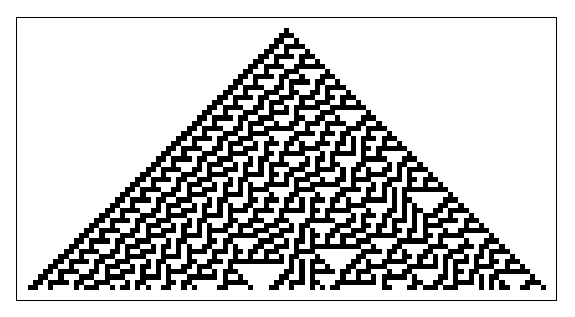
\includegraphics[scale=0.85]{img/rule30.eps}
\caption{Regra 30.}
\label{fig:rule30}
\end{minipage}
\hspace{0.5cm}
\begin{minipage}[b]{0.5\linewidth}
\centering
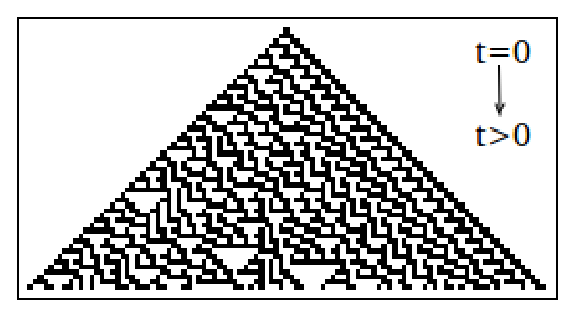
\includegraphics[scale=0.85]{img/rule86.eps}
\caption{Regra 86.}
\label{fig:rule86}
\end{minipage}
\end{figure}

Estudar as classes de equivalência mostra-se importante porque regras locais
equivalentes apresentam o mesmo padrão de complexidade de evolução.

\subsection{Classificação dos autômatos celulares}

\citeonline{wolfram1994} dividiu os ACs elementares em quatro
classes segundo a complexidade do padrão gerado pelo seu comportamento dinâmico,
conforme descrito a seguir:

\begin{description}
\item[Classe 1] A evolução leva a um estado nulo, ou seja, quase todas as condições
iniciais levam ao mesmo estado uniforme.
\item[Classe 2] A evolução leva a um conjunto de estruturas de ponto-fixo ou periódicas.
\item[Classe 3] A evolução leva a um padrão caótico.
\item[Classe 4] A evolução leva a estruturas localizadas complexas.
\end{description}

Os atratores nas classes 1, 2 e 3 são respectivamente análogos aos atratores
de ponto fixo, ciclo limite e caóticos encontrados em sistemas dinâmicos
contínuos. A Figura \ref{fig:classes} mostra exemplos de ACs
das quatro classes de complexidade.

\begin{figure}[htp]
\begin{center}
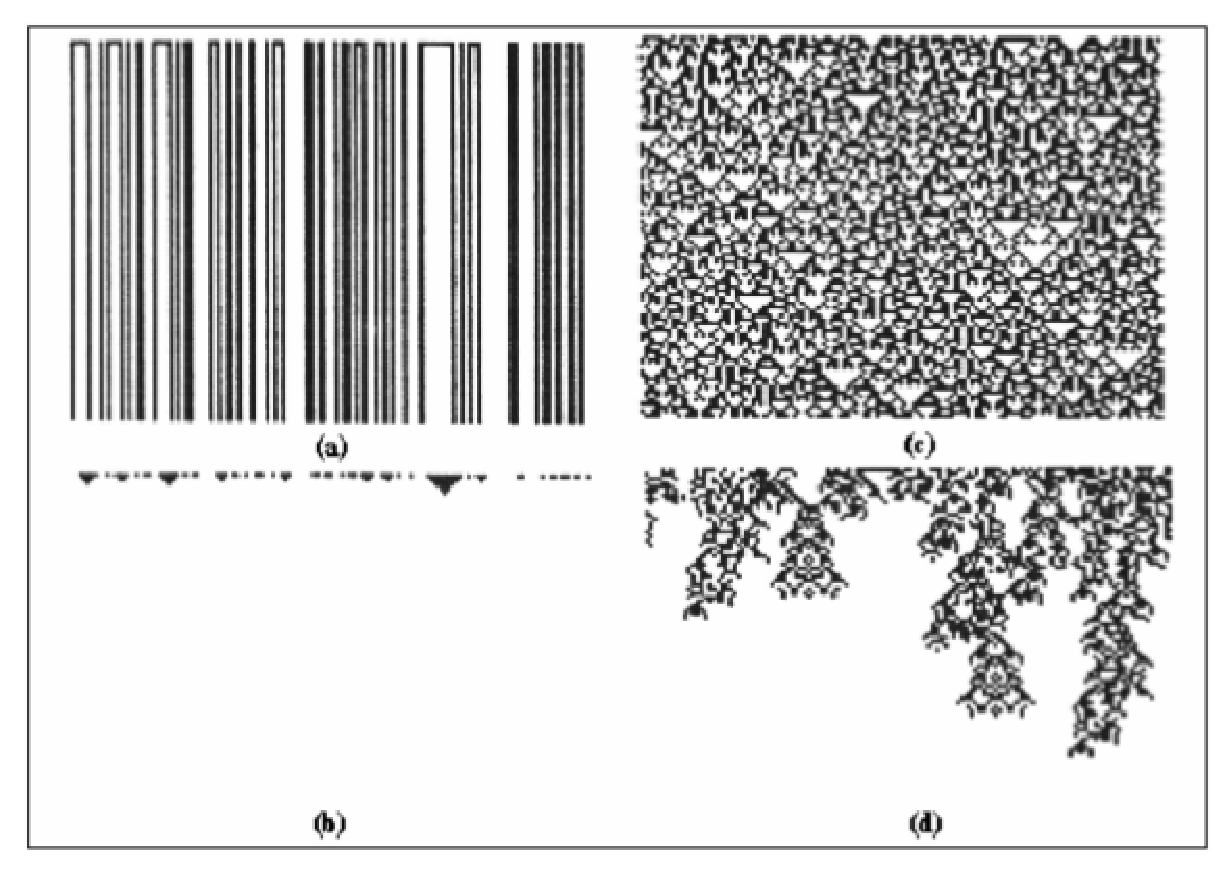
\includegraphics[scale=0.5]{img/classes.eps}
\caption{Classes dinâmicas dos ACs \citecustom{wolfram1984}.
(a) classe 2, (b) classe 1, (c) classe 3 e (d) classe 4.}
\label{fig:classes}
\end{center}
\end{figure}

Trabalhos posteriores se concentraram em formalizar a classificação intuitiva
feita por Wolfram \citecustom{sarkar2000}. \citeonline{li1990} propuseram a seguinte
classificação \citecustom{trafaniuc2004}:

\begin{description}
\item[Regras Nulas] A configuração limite é formada somente por 0s e 1s.

\item[Regras Ponto-Fixo] A configuração limite não se altera ao
reaplicarmos a regra do autômato celular.

\item[Regras Ciclo Duplo] A configuração limite não se altera ao
reaplicarmos a regra do autômato celular duas vezes.

\item[Regras Periódicas] A configuração limite não se altera à aplicação
da regra N vezes, com o tamanho do ciclo N, ou independente ou fracamente
dependente do tamanho do reticulado.

\item[Regras Complexas] Embora a dinâmica limite possa ser periódica,
o intervalo transiente pode ser extremamente longo e, tipicamente,
este intervalo cresce mais que linearmente com o tamanho do sistema.

\item[Regras Caóticas] Produzem dinâmicas não periódicas e se caracterizam
pela divergência exponencial do comprimento do seu ciclo com o tamanho do
reticulado e pela instabilidade com respeito a perturbações.
\end{description}

\subsection{Linguagens formais}

A teoria dos autômatos é o estudo dos dispositivos de computação abstratos,
ou \textit{máquinas}. Antes de existirem computadores, na década de 1930, Alan
Turing estudou uma máquina abstrata que tinha todas as características dos
computadores atuais, pelo menos no que se refere ao quanto eles poderiam 
calcular. O objetivo de Turing era descrever com exatidão o limite entre
o que uma máquina de computação podia fazer e aquilo que ela não podia fazer.

Nas décadas de 1940 e 1950, tipos de máquinas mais simples, que hoje são
conhecidas como \textit{autômatos finitos}, foram estudados por diversos
pesquisadores. Esses autômatos, propostos originalmente no contexto de
modelagem matemática do cérebro, se mostraram extremamente úteis para uma grande variedade
de propósitos. Também no final dos anos 50, o linguista N. Chomsky, iniciou
o estudo de gramáticas formais gerativas, as quais guardam relacionamentos
estreitos com os autômatos abstratos \citecustom{hopcroft2002}.

Linguagens regulares estão entre os tópicos mais antigos em teoria de
linguagens formais. O estudo formal de linguagens regulares
e AFs é datado do início da década de 40, quando máquinas
de estado finito foram utilizadas para modelar conjuntos de neurônios
por McCulloch e Pitts. Desde então, linguagens regulares têm sido
extensivamente estudadas. Resultados das primeiras investigações são,
por exemplo, o teorema de Kleene estabelecendo a equivalência de
expressões regulares e AFs, a introdução de autômatos
com saída por Mealy e Moore e a introdução de AFs não
determinísticos por Rabin e Scott \citecustom{rozenberg1997}.

O elemento básico de uma linguagem é o alfabeto, um conjunto finito de símbolos
utilizados para formar as palavras pertencentes à linguagem. Por exemplo, o
alfabeto $\Sigma = \{0,1\}$ contém os símbolos $0$ e $1$, e todas as palavras
formadas a partir deste alfabeto só poderão conter estes símbolos.

Uma palavra ou cadeia sobre um alfabeto é uma sequência finita de símbolos
pertencentes a este alfabeto. Assim, $011101$ é uma palavra sobre o alfabeto
$\Sigma = \{0, 1\}$. Uma palavra pode não conter nenhum símbolo. Neste caso,
ela recebe o nome de cadeia \textit{vazia}, e é denotada por $\varepsilon$.
O conjunto de todas as palavras não vazias sobre um alfabeto $\Sigma$ é
denotado por $\Sigma^+$, e o conjunto de todas as palavras, incluindo
a cadeia vazia, sobre um alfabeto $\Sigma$ é denotado por
${\Sigma}^+ \bigcup \varepsilon = \Sigma^*$. O comprimento de uma palavra
é o número de símbolos que a forma. Logo, o comprimento da palavra
\emph{abcd} é 4. Denota-se o comprimento de uma cadeia $w$ por
$|w|$; portanto, $|101| = 3$ e $|\varepsilon| = 0$. Alternativamente,
por meio de um isomorfismo natural, uma cadeia $w \in \Sigma^*$ pode ser
considerada uma função $w: \{1,\ldots,|w|\} \mapsto \Sigma$; o
valor de $w(j)$, onde $1 \le j \le |w|$, é o símbolo que ocupa a j-ésima
posição em $w$ \citecustom{lewis2008}.

Dá-se o nome de \textbf{linguagem} a qualquer conjunto de palavras sobre um
alfabeto $\Sigma$, ou seja, a qualquer subconjunto de $\Sigma^*$. Portanto,
$\Sigma^*$, $\varepsilon$ e $\Sigma$ são linguagens. Sendo uma linguagem 
simplesmente um tipo particular de conjunto, pode-se especificar linguagens
finitas enumerando-se todas as suas palavras. Por exemplo, $\{aba, czr, d, f\}$
é uma linguagem sobre $\{a, b, \ldots, z\}$. Entretanto, quando as
linguagens são infinitas, não é possível listar todas as palavras
\citecustom{lewis2008}. Assim, especifica-se linguagens infinitas da seguinte forma:

\begin{center}
$L = \{w \in \Sigma^*: \mbox{ w possui a propriedade P}\}$
\end{center}

\subsection{Autômatos finitos e linguagens regulares}

Segundo \citeonline{hopcroft2002}, um AF é definido por
uma quíntupla $A = (\mathbb{Q},\Sigma,\delta,q_0,\mathbb{F})$, onde:

\begin{description}
\item[$A$] é o nome associado ao AF.
\item[$\mathbb{Q}$] é um conjunto finito de estados.
\item[$\Sigma$] é um conjunto finito de símbolos de entrada
\item[$\delta$] é uma função de transição do tipo $\delta: \mathbb{Q} \times \Sigma \mapsto \mathbb{Q}$.
A função de transição toma um estado e um símbolo de entrada e retorna um novo estado.
$\delta$ também é chamada de \textit{tabela de transição de estados}.
\item[$q_0$] é o estado inicial.
\item[$\mathbb{F}$] é o conjunto de estado finais, com $\mathbb{F} \subseteq \mathbb{Q}$.
\end{description}

O autômato atua lendo símbolos de uma fita de entrada onde cada posição na fita
contém um símbolo. O autômato começa seu processamento no estado inicial $q_0$ e,
a cada símbolo lido da fita de entrada, a função de transição
$\delta: \mathbb{Q} \times \Sigma \mapsto \mathbb{Q}$ define um novo estado como o estado atual.
Quando o processamento da fita de entrada termina, se o estado atual for
um dos estados pertencentes ao conjunto $\mathbb{F}$ de estados finais, a entrada é
considerada aceita, caso o contrário, a entrada é rejeitada. Por exemplo,
considere o seguinte AF:

\begin{center}
$M = \{ \mathbb{Q} = \{A,B\}, \break \Sigma = \{0,1\}, \break
\delta = \{A \times 0 \mapsto A; A \times 1 \mapsto B; B \times 0 \mapsto A; B \times 1 \mapsto B\}, \break
q_0 = A, \break \mathbb{F} = \{B\} \}$
\end{center}

Neste caso, o estado inicial é o estado $A$, e o conjunto de estados finais
é formado pelo estado único $B$. É fácil verificar que este autômato aceita
qualquer palavra sobre o alfabeto $\{0,1\}$ que termine com o símbolo $1$.
Considere a cadeia $00101$. O autômato começa no estado $A$ e lê o primeiro
símbolo $0$, a função $\delta$ possui uma entrada $A \times 0 \mapsto A$,
então o autômato consome o símbolo $0$, avança a fita de entrada e permanece
no estado $A$. Novamente um $0$ é lido, então o estado $A$ é mantido e
avança-se a fita de entrada. Agora o símbolo $1$ é lido, a entrada correspondente
na tabela de transição é $A \times 1 \mapsto B$, então o autômato vai para
o estado $B$. O próximo símbolo da entrada é o $0$, e a entrada correspondente
na tabela de transição é $B \times 0 \mapsto A$, então o autômato vai para o
estado $A$. O último símbolo de entrada é o símbolo $1$, então o autômato vai
para o estado $B$. Como toda a entrada foi consumida e o estado atual $B$
pertence ao conjunto de estados finais $\mathbb{F}$, a cadeia de entrada $00101$ é
aceita.

AFs também podem ser representados graficamente através de
um grafo orientado. Os estados são representados pelos nós do grafo
e os arcos representam as transições de estado. O estado inicial possui
uma seta de entrada e os estados finais possui um círculo duplo. A
Figura \ref{fig:automata} mostra graficamente o autômato anterior.

\begin{figure}[htp]
\begin{center}
\begin{VCPicture}{(0,-2)(3,2)}
\vState[A]{(0,0)}{A} \FinalState[B]{(3,0)}{B}
\Initial{A} %\Final{B}
\ArcL{A}{B}{1} \ArcL{B}{A}{0}
\LoopN{A}{0} \LoopN{B}{1}
\end{VCPicture}
\caption{Autômato finito representado como um grafo orientado.}
\label{fig:automata}
\end{center}
\end{figure}

O AF anteriormente exemplificado é chamado de AF determinístico.
Em um AF determinístico, cada transição na função de transição possui apenas
um único estado objetivo, ou seja, cada entrada da tabela de transição possui a forma
$\delta: \mathbb{Q} \times \Sigma \mapsto \mathbb{Q}$. Nos AFs não
determinísticos, cada entrada na tabela de transição é da forma
$\delta: \mathbb{Q} \times \Sigma \mapsto 2^{\mathbb{Q}}$,
ou seja, para um dado estado e um símbolo de entrada, o número de possíveis
transições pode ser maior que um \citecustom{rozenberg1997}.

A mecânica básica de um AF é simples.
O processamento em um autômato não determinístico é análogo à sua contraparte
determinística, exceto que quando existe uma ambiguidade na transição (existe
mais de um estado objetivo para uma dada entrada), o autômato se replica, tomando
o caminho dos $n$ estados objetivos. A entrada é considerada aceita se, ao
final do processamento, pelo menos uma instância do autômato está em um
estado final.

O conjunto de palavras reconhecidas por um autômato forma a linguagem do
autômato. Seja $M$ um autômato, $L(M)$ constitui sua linguagem. A classe
de linguagens reconhecidas por AFs são as linguagens regulares.
Linguagens regulares podem também ser representadas por meio das chamadas
expressões regulares. 

Dadas as operações:

\begin{description}
\item[União] $A+B=\{x | x \in A \mbox{ ou } x \in B\}$
\item[Concatenação] $AB=\{xy | x \in A \mbox{ e } y \in B\}$
\item[Fechamento de Kleene] $A^*=\{x_1x_2 \ldots x_k | k \ge 0 \mbox{ e cada } x_i \in A\}$.
Adicionalmente também pode-se utilizar a notação $A^+$, que é equivalente a $AA^*$.
\end{description}

Uma expressão $R$ é considerada uma expressão regular \citecustom{sipser1996}
se ela é:

\begin{enumerate}
\item $a$ para algum $a \in \Sigma$
\item $\varepsilon$
\item $\varepsilon$, $1^*\varepsilon=\varepsilon$, $\varepsilon^*=\{\varepsilon\}$, $R\varepsilon=R$
\item $R_1+R_2$, onde $R_1$ e $R_2$ são expressões regulares e
o $+$ representa a união das duas expressões
\item $R_1R_2$, onde $R_1$ e $R_2$ são expressões regulares
\item ${R_1}^*$, onde $R_1$ é uma expressão regular
\end{enumerate}

Por exemplo, a expressão regular do autômato da Figura \ref{fig:automata}
é $(0+1)^*1^+$.

\subsection{Grafos de processo}

Uma importante subclasse das linguagens regulares é a classe de linguagens
de processo. Isto é, para todas as palavras $\omega \in L$, todas as
sub-palavras
$v \in \{s^i \ldots s^{i+j}:s^k=(\omega)_k,i+j\le \|\omega\|,i,j\ge 0\}$
de $\omega$ estão em $L$. Forma-se o fechamento das sub-palavras sub($L$)
de uma linguagem $L$ pela inclusão em sub($L$) de todas as sub-palavras
de cada $\omega \in L$ \citecustom{hanson1992}, ou seja, para cada
cadeia $w \in L$, todas as subcadeias de $w$ também pertencem a $L$.

\begin{definition}
O \textbf{grafo de processo} de uma linguagem de processo $L$ é o grafo
formado permitindo o AF mínimo associado $M(L)$ iniciar em qualquer
estado e marcando todos os estados como de aceitação.
\end{definition}

Todos os estados de um grafo de processo são, então, estados iniciais e de
aceitação.

Claramente linguagens regulares de processo são um conjunto menor do que
linguagens regulares. Por exemplo, a linguagem $L = \{0011\}$ só pode ser
representada por uma linguagem regular.

\subsection{Evolução de um autômato celular}

Uma configuração de um AC pode ser definida por uma concatenação de estados
de células $x_i$, com $-\infty < i < \infty$ para o caso infinito ou
$0 < i < N$ para o caso finito. O conjunto dos estados de todas as células
de um reticulado do AC em um dado passo em sua evolução temporal é chamado de
\textit{configuração global}, e um subconjunto dos estados destas
células define uma \textit{configuração local}.

Linguagens formais consistem do conjunto de palavras formadas a partir de
cadeias de símbolos em um alfabeto finito $\Sigma$ de acordo com regras
gramaticais definidas. Conjuntos de configurações de ACs
podem assim ser considerados como linguagens formais, com cada palavra na
linguagem representando uma configuração do AC. Tais conjuntos
infinitos de configurações são então completamente especificados por
conjuntos finitos de regras gramaticais \citecustom{wolfram1984}.

O conjunto de configurações possíveis em um AC unidimensional depois de $t$
passos de evolução pode ser representado por um conjunto $\Omega^{(t)}$
\citecustom{wolfram1984}.

O seguinte exemplo, retirado de \citecustom{wolfram1984}, ilustra o processo de
geração do AF que representa o conjunto de configurações
possíveis $\Omega^{(t)}$ após $t$ iterações. A construção do AF se baseia no
grafo de De Bruijn \citecustom{debruijn1946,powley2009,mcintosh2009}.
Um grafo de De Bruijn com $m$ símbolos
é um grafo direcionado representando sobreposições entre sequências de símbolos,
onde cada estado possui $m$ arestas chegando e $m$ arestas deixando o estado.
Toda regra elementar pode ser inicialmente representada por um grafo de De
Bruijn de 4 estados, somente as transições mudam para cada regra.

Considere a construção do conjunto $\Omega^{(1)}$ gerado por um passo de
tempo na evolução do AC elementar com uma regra
local $\phi$ dada por (regra número 76):

\begin{equation}\label{eqn:r76}
111 \mapsto 0, 110 \mapsto 1, 101 \mapsto 0, 100 \mapsto 0, 011 \mapsto 1, 010 \mapsto 1,
001 \mapsto 0, 000 \mapsto 0
\end{equation}

O valor $a_i^{(1)}$ de uma célula na posição $i$ em uma configuração
$A^{(1)} = \phi A^{(0)} \in \Omega^{(1)}$ depende da vizinhança de três
células $(a_{i-1}^{(0)},a_i^{(0)},a_{i+1}^{(0)})$ na configuração precedente
$A^{(0)} \in \Omega^{(0)}$. A célula adjacente de $a_{i+1}^{(1)}$ depende da
vizinhança sobreposta $\{a_i^{(0)},a_{i+1}^{(0)},a_{i+2}^{(0)}\}$. A
dependência de $a_{i+1}^{(0)}$ em $a_i^{(0)}$ associada com esta sobreposição
de duas células nas vizinhanças pode ser representada por um grafo de
De Bruijn $g$, conforme
ilustra a Figura \ref{fig:A1}. Os nós no grafo representam as sobreposições
$(a_i^{(0)},a_{i+1}^{(0)})$. Estes nós são agregados por arcos direcionados
correspondentes a vizinhanças de três células. A regra local do AC
$\phi$ da Equação \ref{eqn:r76} define uma transformação para cada
vizinhança de três células, e assim associa um símbolo com cada arco de $g$.
Cada possível caminho através de $g$ corresponde a uma configuração particular
$A^{(0)}$. O sucessor $A^{(1)}$ de cada configuração inicial é dado pela
sequência de símbolos associada com os arcos no caminho. As sequências de
símbolos obtidas seguindo todos os caminhos possíveis através de $g$ assim
correspondem a todas as possíveis configurações $A^{(1)}$ obtidas depois
de um passo de tempo na evolução do AC da Equação \ref{eqn:r76}. O
conjunto completo $\Omega^{(1)}$ pode assim ser representado pelo grafo
$g$. Está claro que nem todas as possíveis sequências de 0s e 1s podem
aparecer nas configurações de $\Omega^{(1)}$. Por exemplo, não existe um
caminho em $g$ que pode incluir a sequência $111$, e assim nenhuma
configuração em $\Omega^{(1)}$ pode conter blocos de células $111$.

\begin{figure}[htp]
\begin{center}
\begin{VCPicture}{(0,-2)(12,8)}
\vState[00]{(0,3)}{A} \vState[01]{(6,6)}{B}
\vState[10]{(6,0)}{C} \vState[11]{(12,3)}{D}
\ArcL{A}{B}{001 \mapsto 0} \LoopW{A}{000 \mapsto 0}
\ArcL{B}{D}{011 \mapsto 1} \ArcL{B}{C}{010 \mapsto 1}
\ArcL{C}{B}{101 \mapsto 0} \ArcL{C}{A}{100 \mapsto 0}
\ArcL{D}{C}{110 \mapsto 1} \LoopE{D}{111 \mapsto 0}
\end{VCPicture}
\caption{O grafo de transição de estados $g$ para um AF
não determinístico que gera as configurações obtidas depois de um passo
de tempo na evolução do AC com a regra número 76.
Possíveis sequências de valores de células são representadas por
caminhos possíveis pelo grafo. Os nós no grafo são rotulados por pares
de valores iniciais das células; os arcos então correspondem a triplas
de valores iniciais das células. Cada tripla é mapeada sob a regra 76
para um valor particular da célula. O grafo com arcos rotulados por estas
células correspondem a todas as configurações possíveis obtidas depois
de um passo de tempo \citecustom{wolfram1984}.}
\label{fig:A1}
\end{center}
\end{figure}

O grafo $g$ da Figura \ref{fig:A1} pode ser considerado como um grafo
de transição de estados para um AC o qual gera a linguagem
formal $\Omega^{(1)}$. Cada nó de $g$ corresponde a um estado do
AF, e cada arco a uma transição no AF, ou
equivalentemente a uma regra  de produção na gramática representada pelo
AF. O conjunto $\Omega^{(1)}$ assim forma uma linguagem
regular.

\subsection{Configuração inicial de um autômato celular}

O espaço de configurações iniciais $\Omega^{(0)}$ de um AC
elementar pode ser qualquer combinação de sequências de 0s e 1s
representando os estados iniciais das células. O AF
que representa tal sequência pode ser visualizado na Figura
\ref{fig:initconfigautomaton}, e sua representação em formato de
grafo de processo na Figura \ref{fig:initconfigmathematica}.

\begin{figure}[htp]
\begin{center}
\begin{VCPicture}{(0,-2)(3,2)}
\FinalState[A]{(0,0)}{A}
\Initial{A}
\LoopN{A}{0,1}
\end{VCPicture}
\caption{Possíveis configurações iniciais representadas por um AF
determinístico. É fácil perceber que o autômato aceita qualquer sequência de
0s e 1s.}
\label{fig:initconfigautomaton}
\end{center}
\end{figure}

\begin{figure}[htp]
\begin{center}
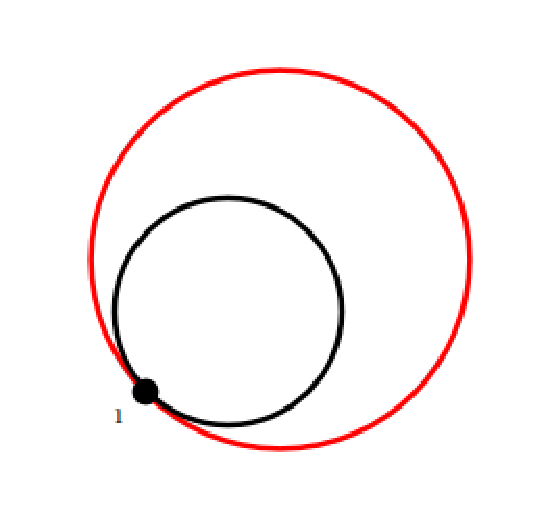
\includegraphics[scale=0.3]{img/InitialConfig.eps}
\caption{Grafo de processo representando as possíveis configurações
iniciais. Arcos vermelhos representam transições em 0 e arcos
pretos representam transições em 1.}
\label{fig:initconfigmathematica}
\end{center}
\end{figure}

Na representação do \textit{Mathematica}, transições em 0 são
representadas por arcos vermelhos e transições em 1 são
representadas por arcos pretos.

\subsection{Funções NetCAStep, TrimNet e MinNet}

\emph{NetCAStep}, \emph{TrimNet} e \emph{MinNet} \citecustom{wolfram2002} são
funções desenvolvidas no \textit{Mathematica} para gerar AFs
que representam a evolução para um passo de tempo de um AC
elementar.

Dado um grafo de processo relacionado à configuração do AC para
um instante de tempo $t$, a função \emph{NetCAStep} \citecustom{wolfram2002}
retorna um AF relacionado ao instante de tempo $t+1$
\citecustom{miki2006}.

A função \emph{NetCAStep} gera como saída uma lista de transições
de estados correspondente a um AF não determinístico.
Sobre a lista de transições de estado resultante da função
\emph{NetCAStep} é aplicada a função \emph{MinNet}, que, por sua vez,
gera um AF determinístico mínimo equivalente ao autômato gerado por
\emph{NetCAStep}.

A função \emph{TrimNet} transformação do AF de saída da \emph{MinNet}
em um grafo de processo.

\newpage

\section{Complexidade de linguagens regulares de autômatos
finitos elementares}\label{sec:complexity}

O conjunto de possíveis configurações globais de um AC elementar pode ser
representado por um AF para um passo de tempo finito. Para
o caso $t \rightarrow \infty$, o conjunto de configurações globais pode ou
não ser representado por um AF. Diversos trabalhos trataram de estudar e
caracterizar o comportamento limite de ACs.

O comportamento limite de um AC pode ser definido por uma linguagem
formal dentro da hierarquia de Chomsky. \citeonline{hurd1987} apresentou
exemplos de ACs para os quais o conjunto limite eram linguagens não
regulares. Exemplos adicionais foram apresentados em \citecustom{hurd19902}.
\citeonline{hurd1987}também provou que o problema de determinar se uma
dada cadeia aparece no conjunto limite de um AC é indecidível.
Uma prova alternativa utilizando uma abordagem topológica foi demonstrada
por \citecustom{culik1989}.  \citeonline{hurd1990} construiu um AC cuja
linguagem limite não é recursivamente enumerável.

\citeonline{culik1988} formalizaram a classificação de ACs proposta por
\citecustom{wolfram2002}. Com a formalização, conseguiram provar que é
indecidível determinar a qual classe um determinado AC pertence, e que
ACs que evoluem para um estado quiescente não necessariamente possuem
comportamento limite descrito por uma linguagem regular.

\citeonline{zhisong2001}, utilizando dinâmica simbólica e teoria de
linguagens formais, provou que o conjunto limite da regra 122 é,
pelo menos, sensível ao contexto. \citeonline{zhisong2005} provaram que
o comportamento limite da regra 22 não é regular.

\citeonline{kurka2000} analisaram a probabilidade do aparecimento de
determinadas estruturas conforme $t \mapsto \infty$ para as regras
18, 54, 62 e 184, e também compararam este conceito probabilístico
com o conceito de atratores, tanto do ponto de vista topológico
quanto de teoria de medidas.

O encadeamento das funções NetCAStep, MinNet
e TrimNet rende um grafo de processo que representa o conjunto de
configurações globais para um passo de tempo finito, conforme ilustra
a Figura \ref{fig:net}.

\begin{figure}[htp]
\begin{center}
\input net.tex
\centerline{\box\graph}
\caption{Sequência de utilização das funções NetCAStep, MinNet e TrimNet.}
\label{fig:net}
\end{center}
\end{figure}

Conforme avançam-se os passos de tempo, a tendência é que o conjunto de 
configurações fique mais restrito e, como consequência, o grafo torne-se
mais complexo. A Figura \ref{fig:r11t} mostra os grafos de processo de
4 passos de tempo para a regra 11. Nota-se que, com o passar do tempo,
o número de estados e transições aumenta, em decorrência da maior
restrição de configurações possíveis. \citeonline{wolfram1984} propôs
este aumento de complexidade do grafo como medida de complexidade da
regra, ou seja, a complexidade da regra é proporcional ao aumento do número
de estados e transições dos grafos dos sucessivos passos de tempo.

\begin{figure}[htp]
\begin{center}
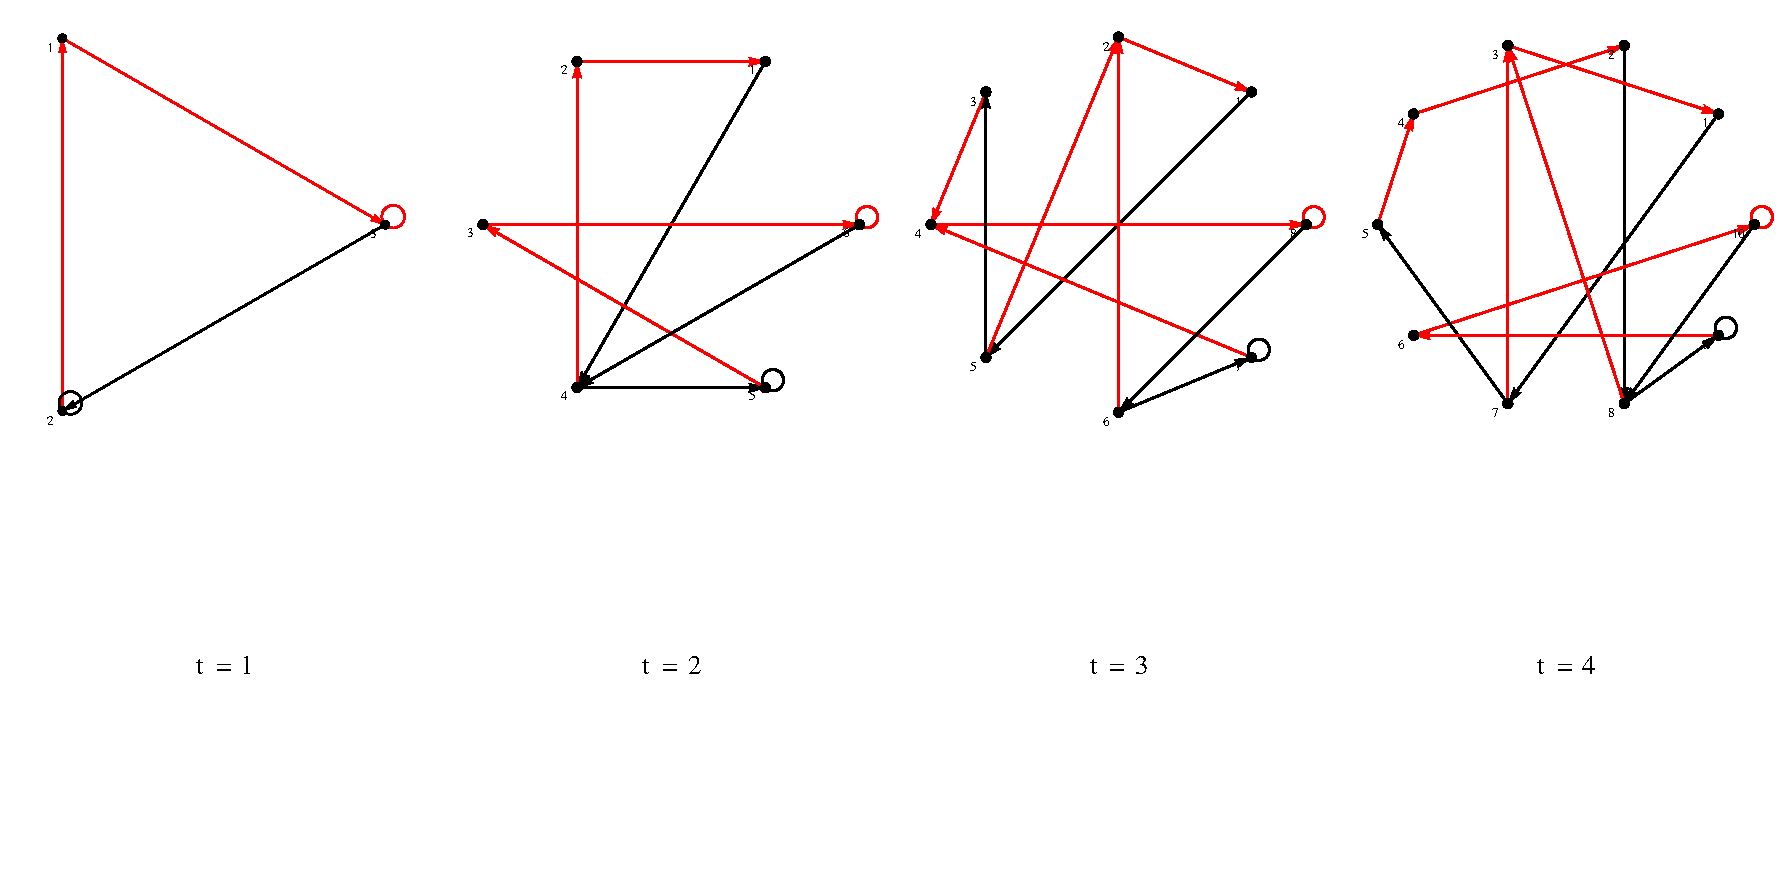
\includegraphics[scale=0.5]{img/Rule11.eps}
\caption{Grafos de processo para 4 passos de tempo da regra elementar 11.}
\label{fig:r11t}
\end{center}
\end{figure}

Conforme já mencionado, o conjunto de configurações globais de uma regra
unidimensional de um AC pode ou não ser representada por um grafo de
processo. É importante ressaltar que esta abordagem limita-se à condição
de contorno não periódica. Para condição de contorno periódica, este grafo
pode não existir para uma determinada regra, mesmo existindo na condição de
contorno não periódica. Como exemplo, segue uma prova de que não é possível
representar o comportamento limite da regra 184 por meio de grafos de processo
para condição de contorno periódica.

\begin{proposition}
Não é possível representar o comportamento limite da regra 184 por meio de
um grafo de processo para condição de contorno periódica.
\end{proposition}

\begin{proof}
Considera-se $L$ como sendo a linguagem limite da regra 184. Considera-se $G$
como sendo o grafo de processo que reconhece $L$. Admite-se também a
cadeia $w = 000101$ pertencente a $L$. Defini-se então $v = 100010$.
$v$ também pertence a $L$ uma vez que é igual
a $w$ com um deslocamento à direita, logo $v$ também é reconhecida por $G$.
Dado $v' = 10001$, uma sub-cadeia de $v$, da definição de
linguagens regulares de processo e grafos de processo, $v'$ também é
reconhecida por $G$, mas não pode pertencer a $L$, porque $v'$ é
a cadeia $11000$ deslocada, e sabe-se que essa string não
faz parte do conjunto limite da regra 184.
\end{proof}

Pode-se imaginar que, para os casos em que o grafo
limite existe, a execução do encadeamento das funções NetCAStep, MinNet e
TrimNet por um período suficiente de tempo levará ao grafo limite, conforme
se exemplifica na Figura \ref{fig:r8t}. Mas existem regras em que esta
convergência não ocorre, como a regra 128, mesmo seu comportamento limite
sendo conhecido (Figura \ref{fig:limit184}) \citecustom{wolfram1984}.

\begin{figure}[htp]
\begin{center}
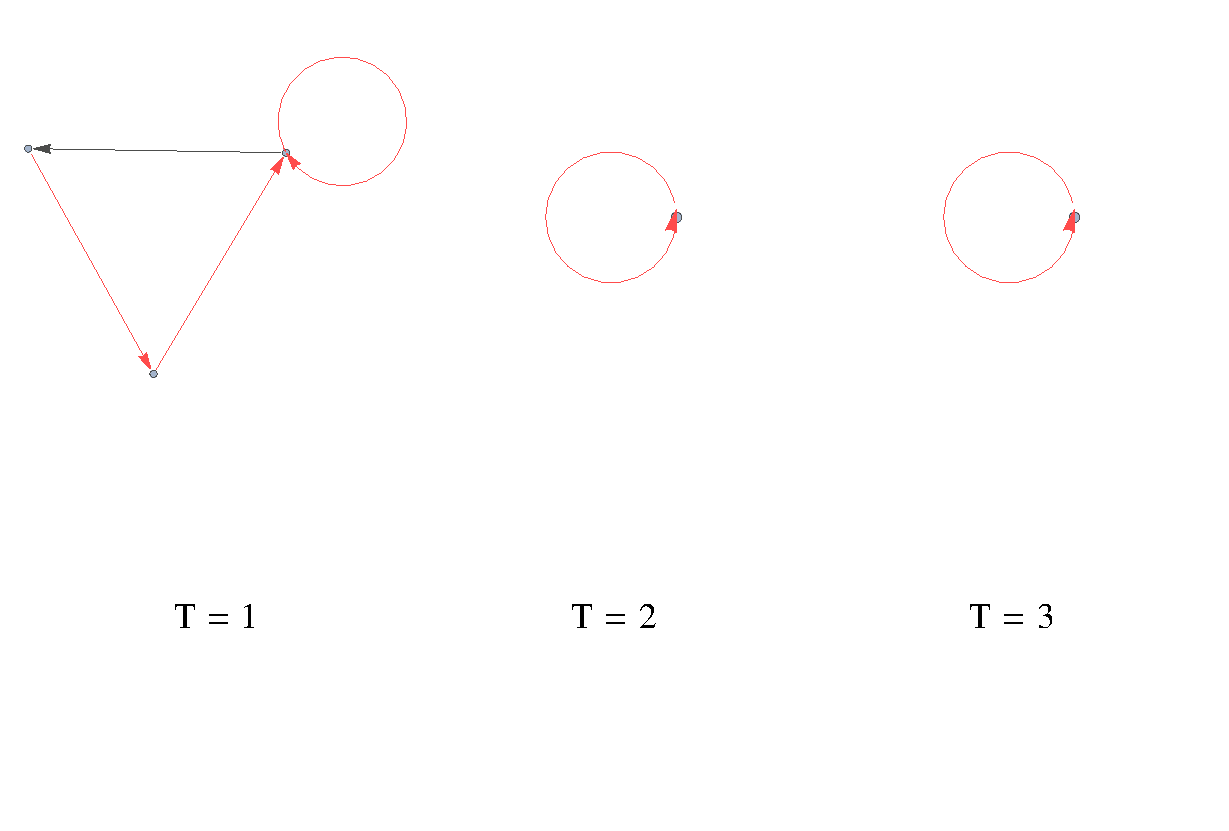
\includegraphics[scale=0.5]{img/Rule8.eps}
\caption{Convergência da regra 8 para o grafo de processo limite.}
\label{fig:r8t}
\end{center}
\end{figure}

\begin{figure}[htp]
\begin{center}
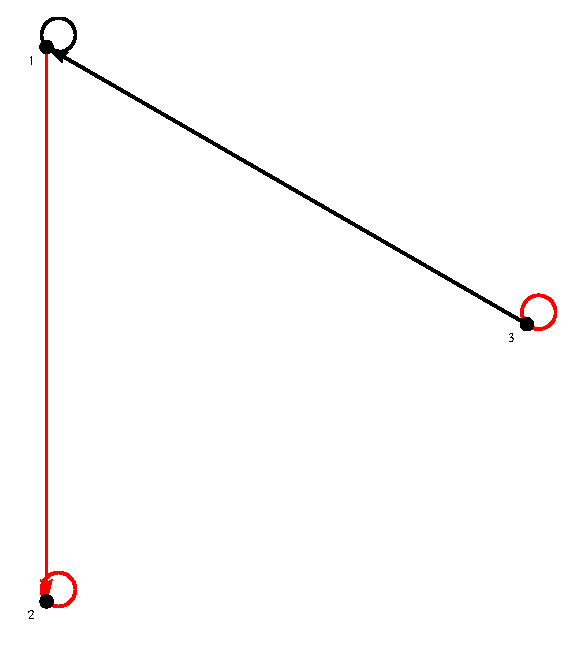
\includegraphics[scale=0.5]{img/limit128.eps}
\caption{Grafo de processo limite da regra 128.}
\label{fig:limit128}
\end{center}
\end{figure}

A explicação do porque regras como a 128 não convergirem e a busca por um
método algorítmico que gerasse o comportamento limite de tais regras foi
a motivação do trabalho de \citecustom{trafaniuc2004} e, posteriormente,
\citecustom{miki2006}.

\citecustom{trafaniuc2004} procurou isolar aquelas regras
que possuem crescimento estruturado, ou seja, em que se pode observar
estruturas comuns nos sucessivos passos de tempo. Primeiramente, sobre as
256 regras elementares, foi aplicado um algoritmo para seleção de regras
que apresentam grafos com complexidade crescente a cada passo de tempo. O
algoritmo é ilustrado na Figura \ref{fig:rulesel}.

\begin{figure}[htp]
\begin{center}
\input rulesel.tex
\centerline{\box\graph}
\caption{Algoritmo de seleção de regras \citecustom{trafaniuc2004}.}
\label{fig:rulesel}
\end{center}
\end{figure}

O algoritmo divide as regras em dois grupos \citecustom{trafaniuc2004}:

\begin{description}
\item[Grupo 1:] Regras que apresentam crescimento de complexidade no AF
limite a cada passo de tempo, e o método é interrompido quando o
número máximo de passos de execução for atingido.
\item[Grupo 2:] Regras que deixam de apresentar crescimento de complexidade no
AF em até cinco passos de tempo.
\end{description}

Na prática, o que o algoritmo faz é isolar as regras que convergem para o
grafo limite (Grupo 2) das que não convergem (Grupo 1). 

Foram então analisadas as estruturas de crescimento de complexidade das regras
do Grupo 1, primeiro manualmente e, depois, automaticamente por meio do
seguinte método \citecustom{trafaniuc2004}:

\begin{enumerate}\label{sec:mikialgo}
\item Gerar os grafos das regras de transição, para dois passos de tempo
consecutivos, $t$ e $t+1$, de uma regra do espaço elementar.

\item Gerar todos os possíveis subgrafos do passo de tempo $t+1$ que tenham
o mesmo número de estados que o grafo do passo de tempo $t$.

\item Selecionar todos os subgrafos gerados com base no passo de tempo $t+1$
que se encaixam perfeitamente no grafo do passo de tempo $t$. Ou seja,
selecionar os subgrafos gerados no passo dois, que também são subgrafos do
grafo no tempo $t$.

\item Realizar uma operação de diferença entre o grafo de $t$ e todos os
subgrafos de $t+1$ selecionados no passo três, com o mesmo número de nós. O
subgrafo que apresentar a menor diferença no número de transições de estados
é selecionado. No caso de empate, o primeiro subgrafo é selecionado.
\end{enumerate}

O algoritmo selecionou 26 regras que apresentavam padrão
de crescimento do AF gerado para os sucessivos passos de tempo na evolução
do AC. O trabalho deduziu a expressão de crescimento da regra 184, inclusive
um método para a obtenção do AF de tempo $t$. Após, o trabalho fez as mesmas
análises para as outras 25 regras. Do total das 26 regras, 16 regras
apresentaram relações entre passos de tempo distintos, sendo elas: 43, 113,
128, 132, 136 140, 142, 162, 168, 176, 184, 192, 196, 212, 224 e 232. Destas
16 regras, para 12 delas foram encontradas as expressões que caracterizam o
crescimento dos grafos de processo de acordo com o passo de tempo, sendo
apresentado o método de obtenção do grafo de processo de passo $t$ para cada uma.
O trabalho chegou à conclusão que são necessárias duas
propriedades para caracterização do grafo de processo de uma regra
\citecustom{trafaniuc2004}:

\begin{enumerate}
\item O crescimento do número de estados do grafo de processo deve ser
proporcional ao passo de tempo, ou seja, o número de estados cresce
a cada passo de tempo.

\item Os grafos de processo para passos de tempo distintos devem possuir uma
relação de crescimento, conforme descrito anteriormente.
\end{enumerate}

\citeonline{trafaniuc2004} reconstruiu a tabela de complexidade de
\citecustom{wolfram1994}, preenchendo novas lacunas na tabela. Também
encontrou alguns valores divergentes em relação à tabela original, embora
não tenha mencionado nada em relação a tal discrepância.
\citeonline{miki2006}, posteriormente, identificou que a descrição da função
MinNet estava errada em \citecustom{wolfram2002}, que apontava o primeiro
estado como sendo o estado inicial no autômato gerado pela função, mas na
verdade o último estado é o que representa o estado inicial, e atribuiu
a esse fato como possível causa das diferenças entre as tabelas de
\citecustom{trafaniuc2004} e \citecustom{wolfram1994}.

\citeonline{miki2006} automatizou o processo manual de análise de crescimento
de AFs desenvolvido por \citeonline{trafaniuc2004} por meio de uma operação
de diferença de grafos. Com os resultados, o trabalho passou a focar na análise
da regra 184 no objetivo de obter o autômato limite. O autômato limite
foi construído manualmente como referência, conforme mostrado na Figura
\ref{fig:limit184}.

\begin{figure}[htp]
\begin{center}
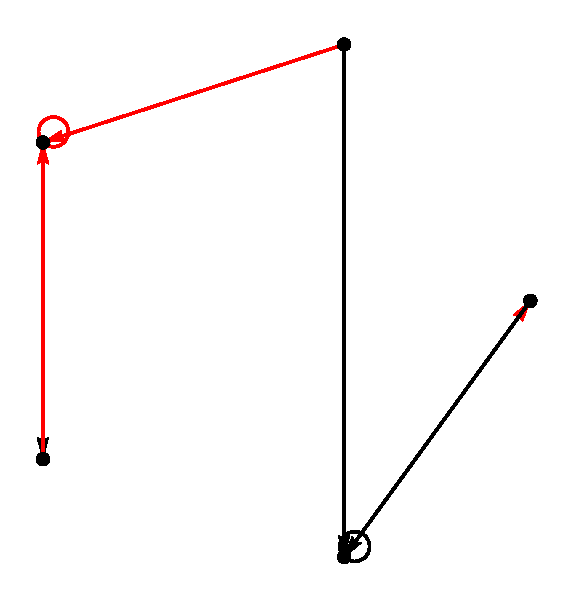
\includegraphics[scale=0.8]{img/limit184.eps}
\caption{Grafo limite da regra 184 segundo \citecustom{miki2006}.}
\label{fig:limit184}
\end{center}
\end{figure}

\citeonline{miki2006} identificou que os grafos de processo dos sucessivos passos de
tempo da regra são assimétricos, mas o grafo de processo limite é simétrico, e não
conseguiu achar uma operação que faça essa transformação de simetria;
não conseguindo, assim, encontrar o grafo de processo limite da regra 184
partindo-se dos grafos de processo intermediários.

\citeonline{miki2006} conseguiu, por meio da automação do processo de análise,
obter as expressões de crescimento das regras 11, 14, 35, 50, 70 e 81, que
\citecustom{trafaniuc2004} não tinha conseguido.

\subsection{Problemas encontrados no trabalho de
\citecustom{trafaniuc2004}}\label{sec:problem}

Tanto \citecustom{trafaniuc2004} quanto \citecustom{miki2006} basearam seus
respectivos trabalhos nas funções NetCAStep, MinNet e TrimNet.
\citeonline{trafaniuc2004} usava a saída da função NetCAStep como entrada
para a função TrimNet, cuja saída era usada como entrada da função
MinNet, que então realimentava a função NetCAStep. Como primeira
consequência (e já apontado em \citecustom{miki2006}),
\citeonline{trafaniuc2004} trabalhou com AFs determinísticos, e não com
grafos de processo como descreveu. \citeonline{trafaniuc2004} realimentou
a função NetCAStep com a saída da função MinNet, enquanto
\citeonline{miki2006} utilizou a saída da função TrimNet para realimentar
a função NetCAStep. A Figura \ref{fig:net-miki} mostra o encadeamento de
chamadas das funções NetCAStep, MinNet e TrimNet de acordo com
\citecustom{miki2006}.

\begin{figure}[htp]
\begin{center}
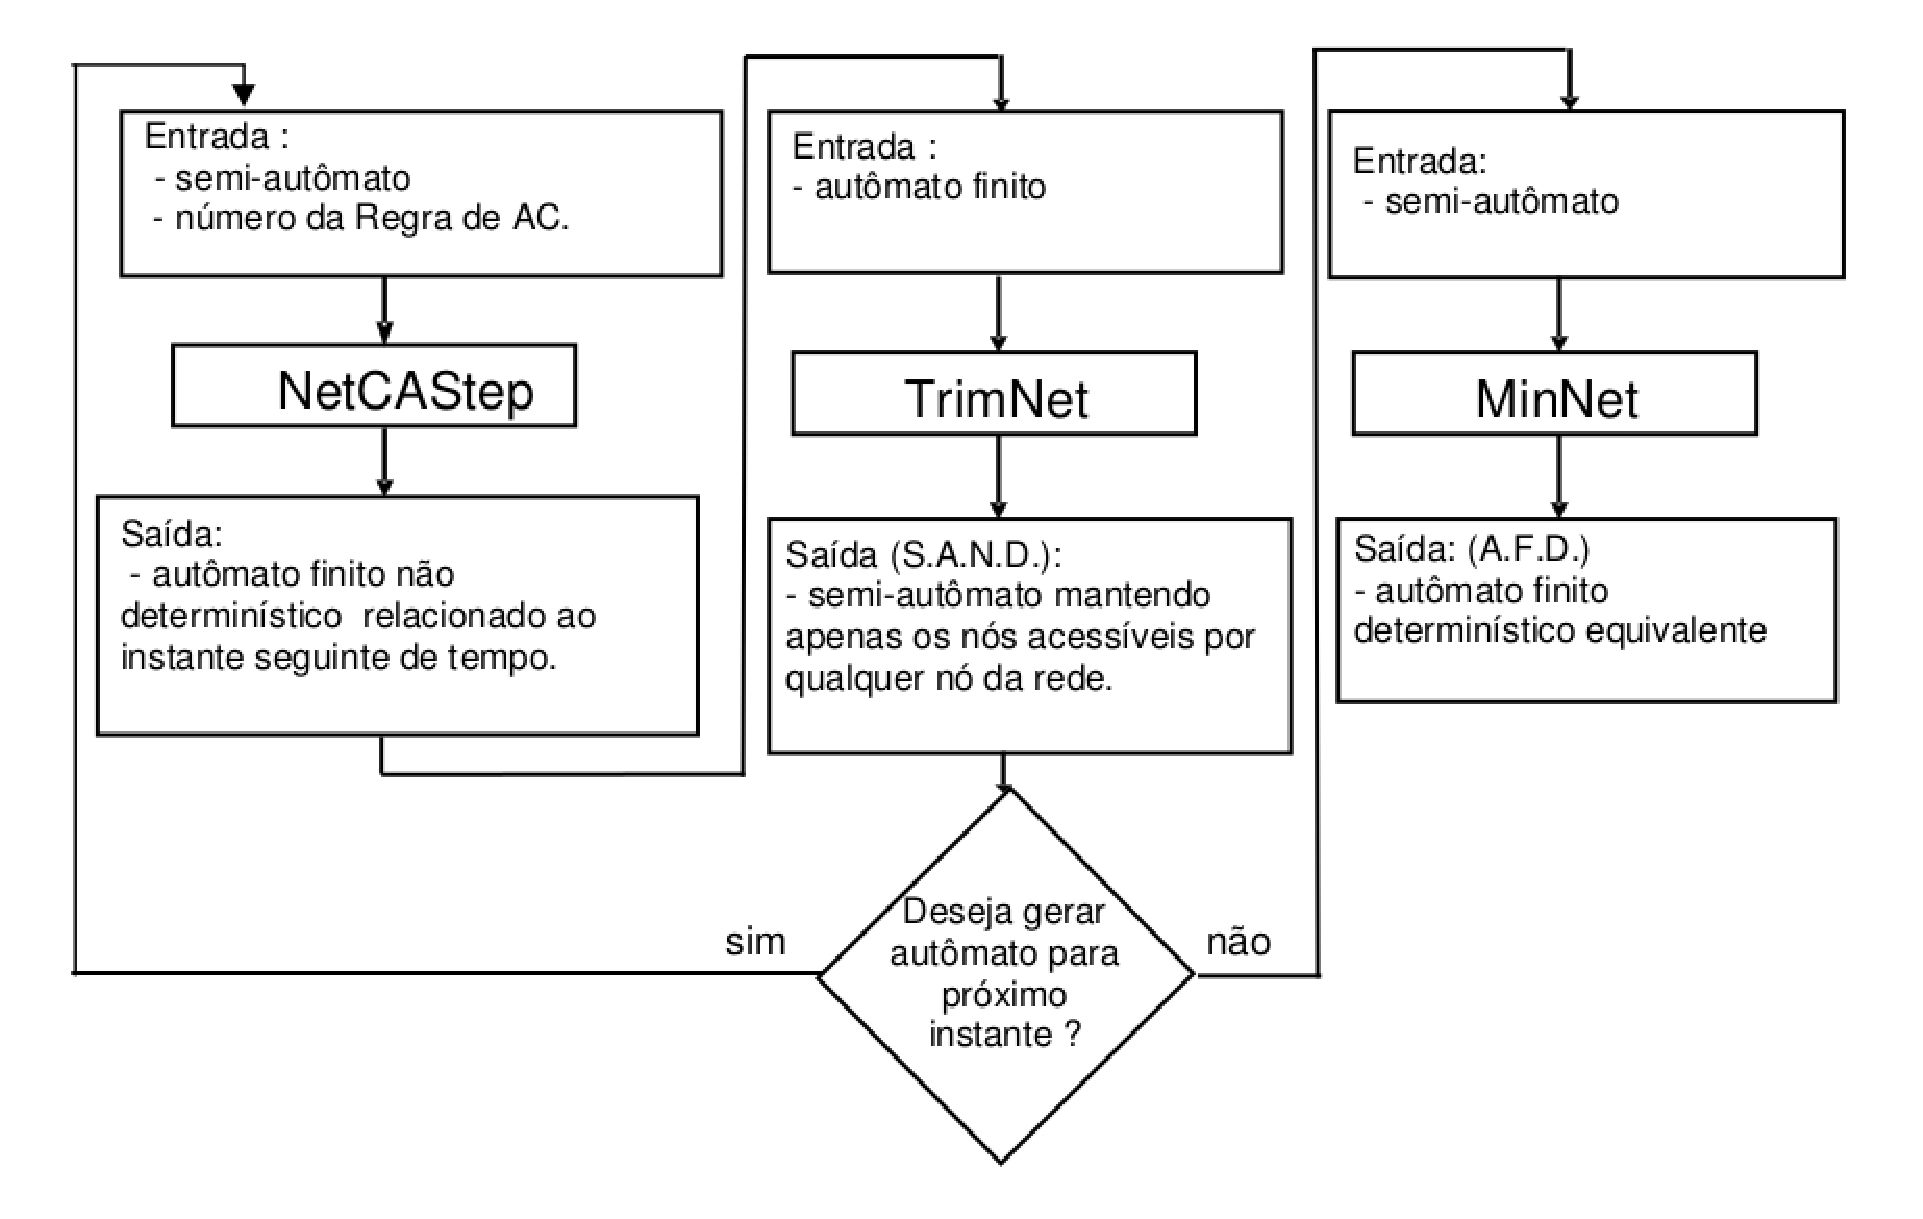
\includegraphics[scale=0.5]{img/net-miki.eps}
\caption{Sequência de chamada das funções NetCAStep, MinNet e TrimNet de
acordo com \citecustom{miki2006}.}
\label{fig:net-miki}
\end{center}
\end{figure}

De acordo como está descrito em
\citecustom{wolfram2002}, nenhuma das duas formas estaria correta e,
teoricamente, o modo como foram executadas leva a um comportamento indefinido,
sendo a forma como apresentada na Figura \ref{fig:net} o modo correto de
encadeá-las e realimentá-las.

Com isso, a construção da tabela de \citecustom{wolfram1994} foi novamente
refeita. A nova tabela e a discussão dos resultados são apresentados na
Seção \ref{sec:table}.

Outro ponto é que descobriu-se que o algoritmo de seleção de regras com
crescimento estruturado apresentado na Seção \ref{sec:mikialgo} gera falsos
negativos, ou seja, algumas regras que apresentam crescimento estruturado
não são selecionadas pelo algoritmo. Este problema foi descoberto durante
a análise da regra 32. Comparando-se os grafos de processo das regras
32 (Figura \ref{fig:r32t}) e 128 (Figura \ref{fig:r128t}), repara-se que
ambos são muito semelhantes, mas a regra 128 é selecionada pelo algoritmo,
enquanto a regra 32 é descartada.

\begin{figure}[htp]
\begin{center}
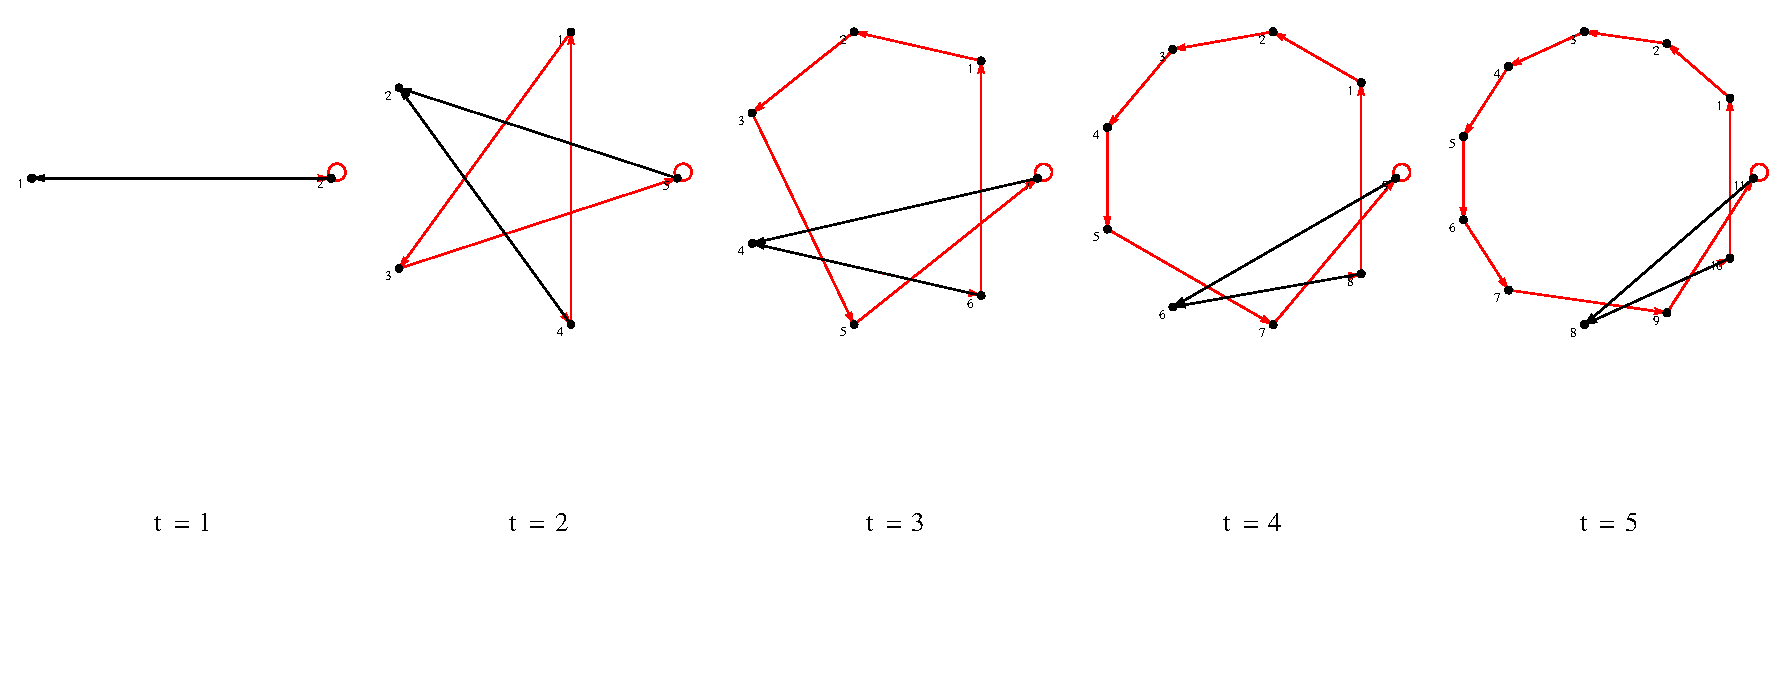
\includegraphics[scale=0.55]{img/Rule32.eps}
\caption{Sequência de grafos de processo da regra 32.}
\label{fig:r32t}
\end{center}
\end{figure}

\begin{figure}[htp]
\begin{center}
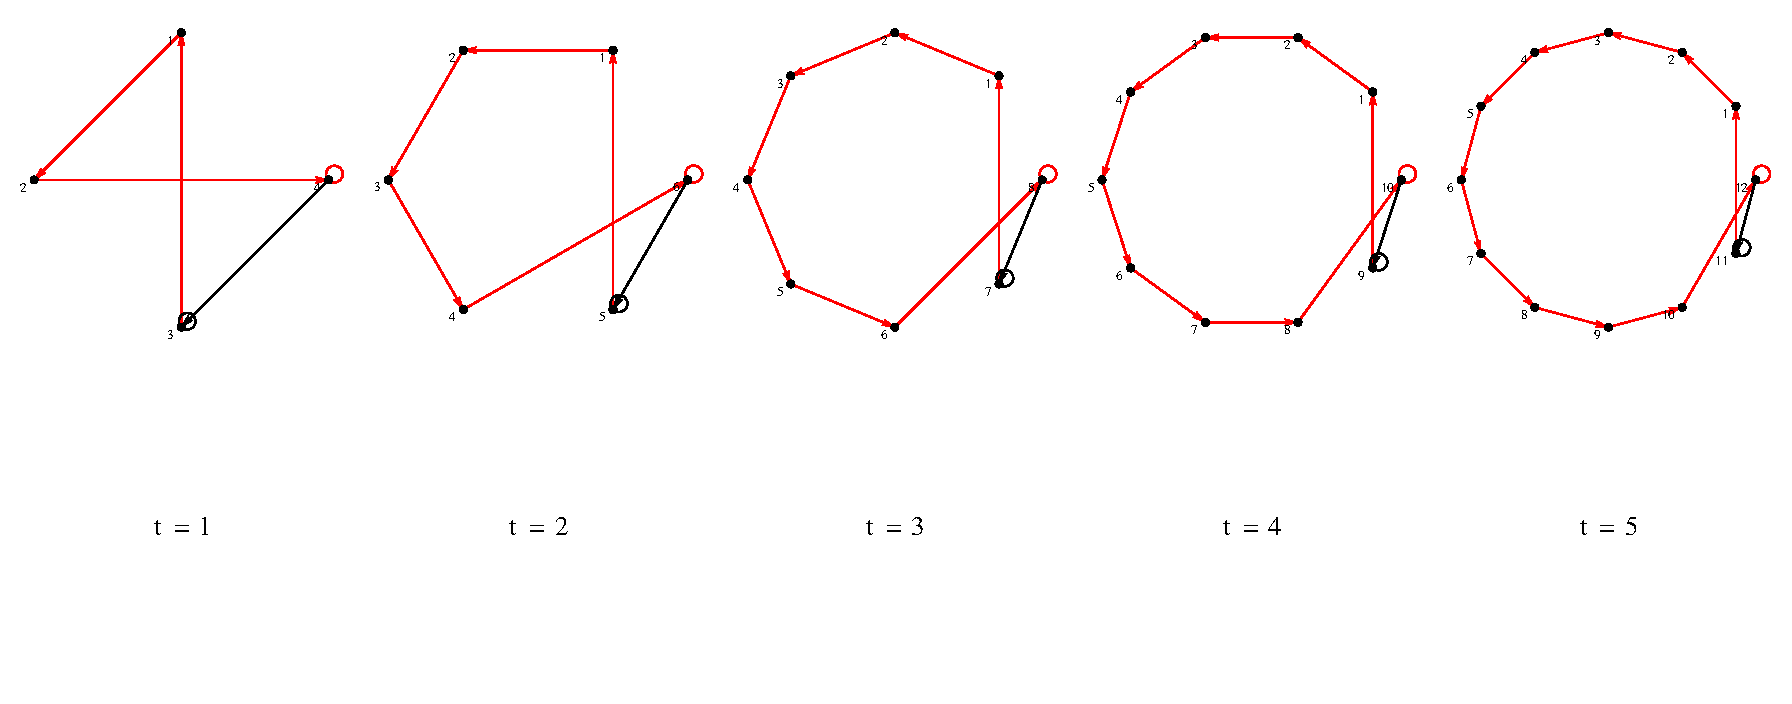
\includegraphics[scale=0.55]{img/Rule128.eps}
\caption{Sequência de grafos de processo da regra 128.}
\label{fig:r128t}
\end{center}
\end{figure}

Nota-se que ambas as regras possuem grafos de processo com a mesma estrutura geral:
uma pequena estrutura imutável é formada no canto inferior direito, e existe
uma sequência de transições que parte desta estrutura e retorna à mesma, com
a distância deste caminho aumentando a cada passo de tempo.

Após uma extensa análise da implementação do algoritmo, descobriu-se que o
problema estava no comportamento da função \textit{GraphDifference} do
software \textit{Mathematica}, utilizada na implementação do algoritmo.
O algoritmo original utilizava a antiga versão do pacote
\textit{Combinatorica}, mas testes mostraram que a versão mais recente da
função, integrada ao núcleo do \textit{Mathematica}, apresenta o mesmo
comportamento. A Figura \ref{fig:gd1} mostra a operação
\textit{GraphDifference} entre dois grafos de processo de passos de tempo
consecutivos da regra 32.

\begin{figure}[htp]
\begin{center}
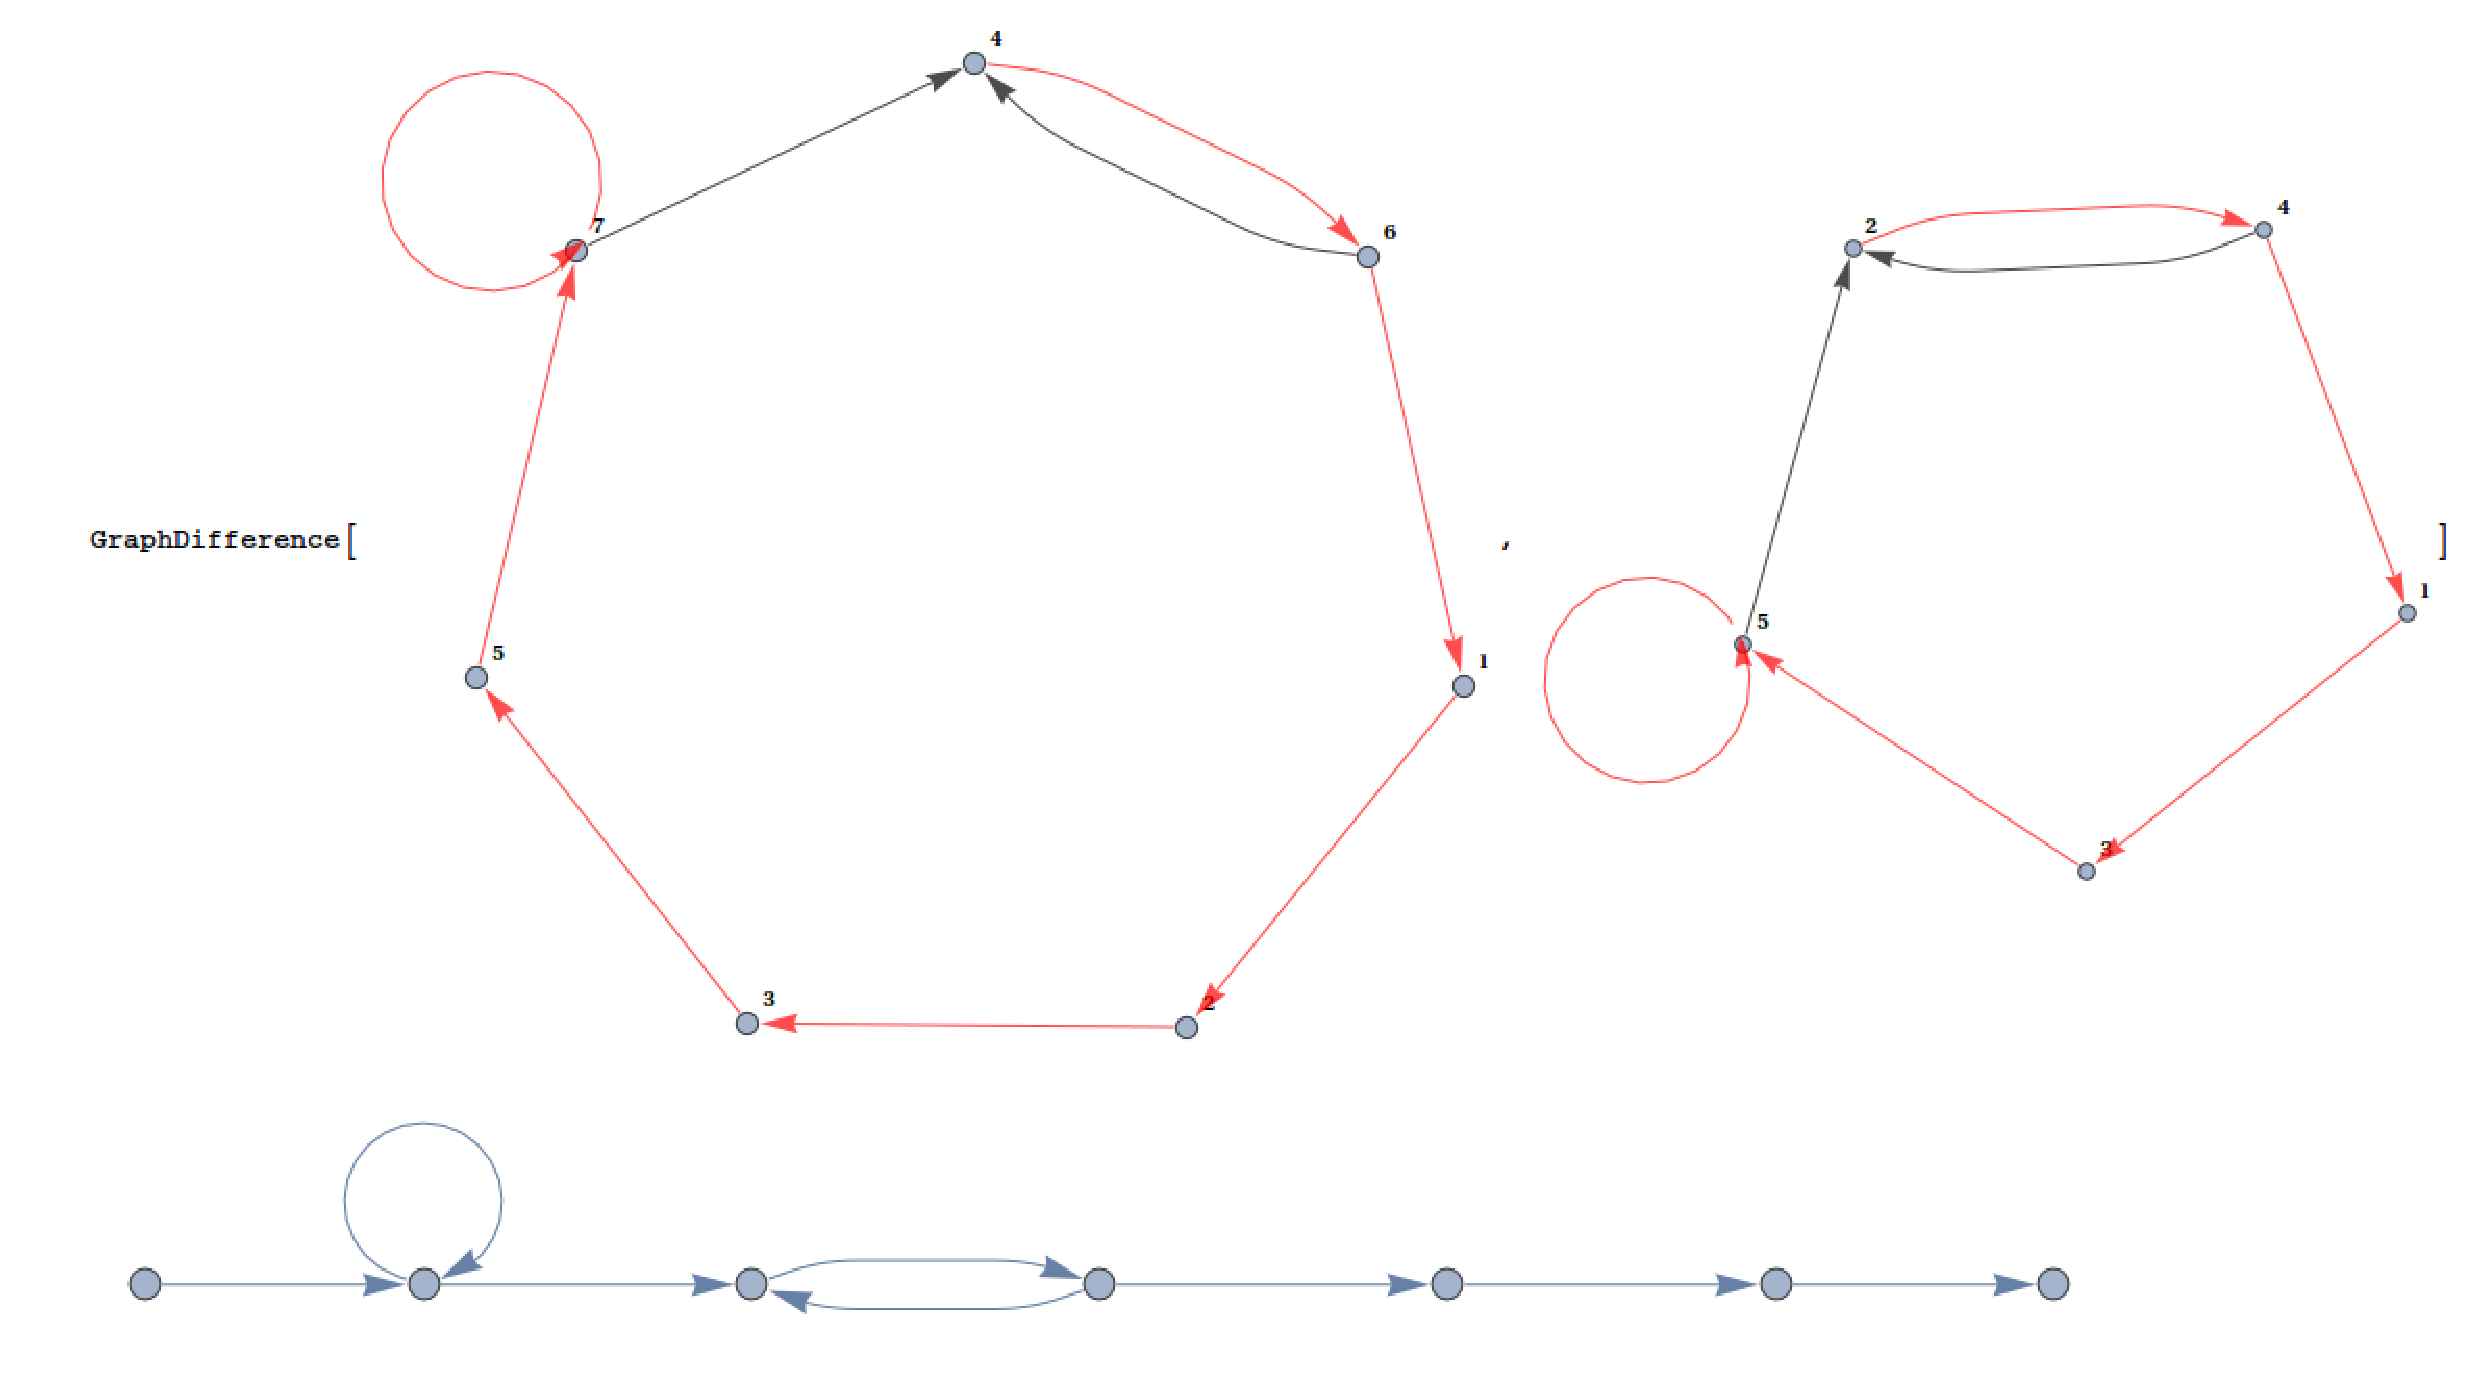
\includegraphics[scale=0.4]{img/GraphDifference1.eps}
\caption{Função \textit{GraphDifference} para dois grafos de processo
adjacentes da regra 32.}
\label{fig:gd1}
\end{center}
\end{figure}

Agora, a Figura \ref{fig:gd2} mostra o que ocorre quando se muda a numeração
dos vértices do primeiro grafo.

\begin{figure}[htp]
\begin{center}
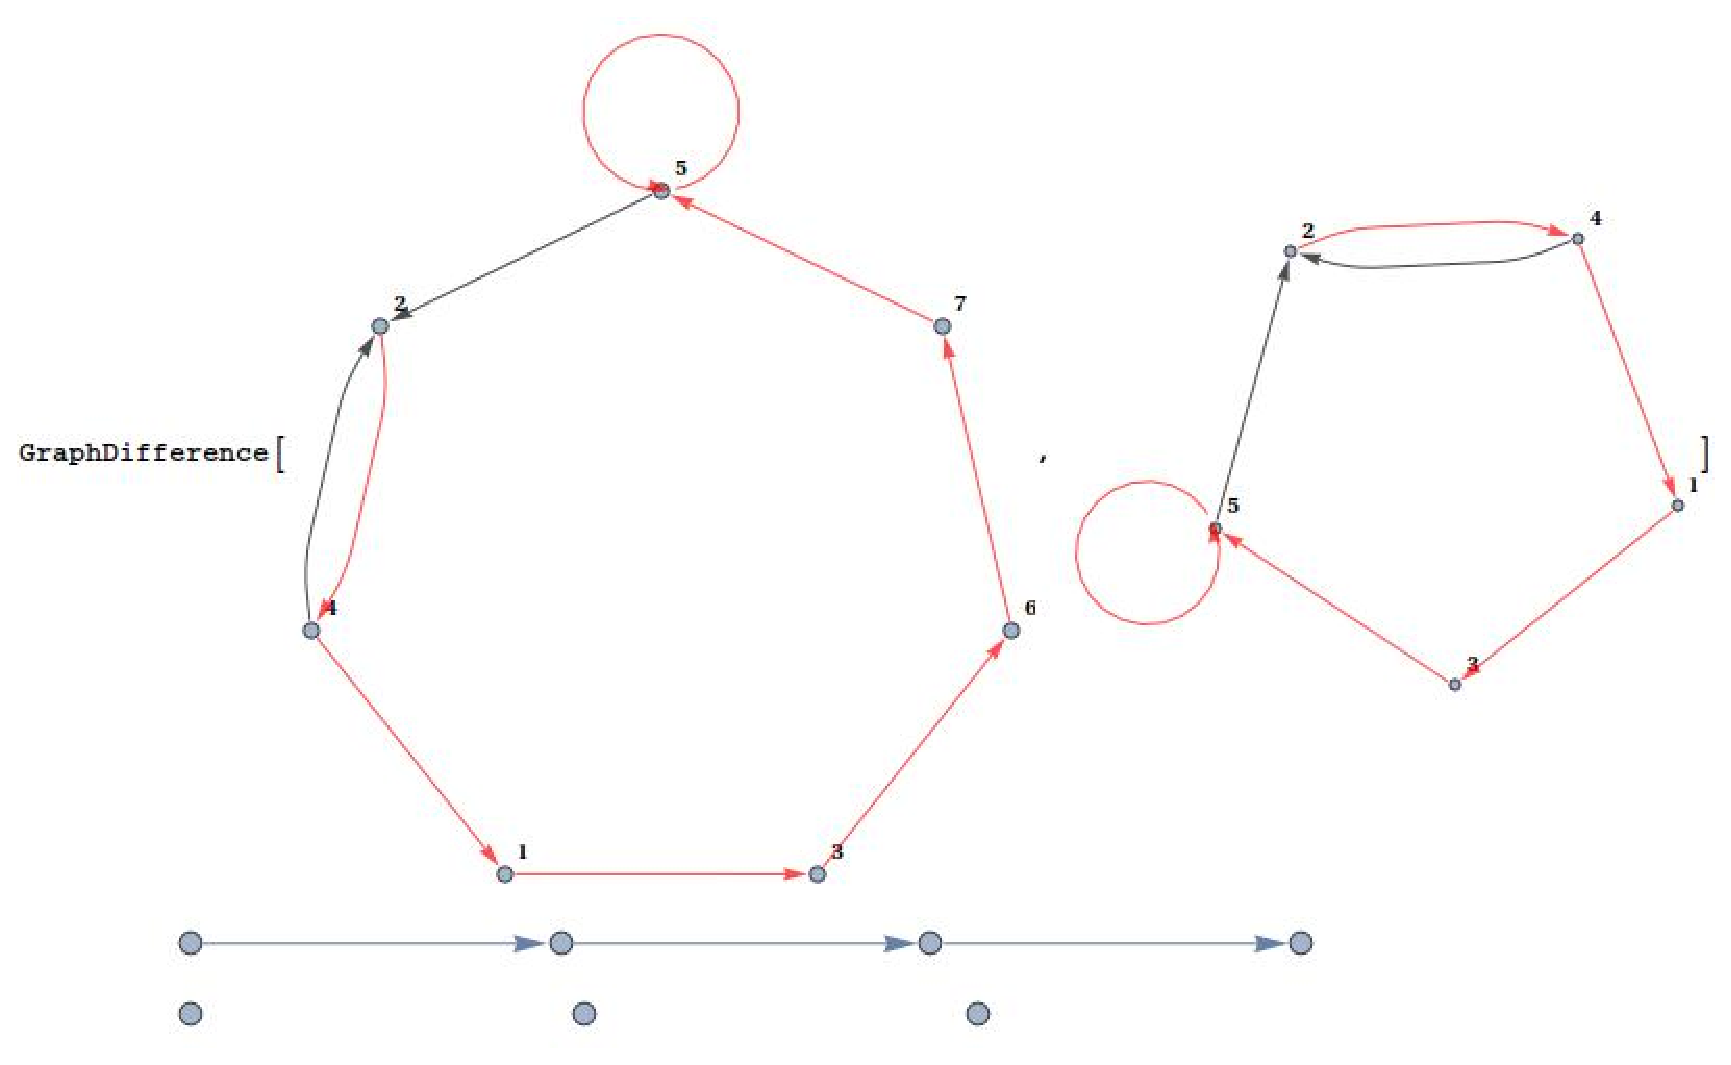
\includegraphics[scale=0.4]{img/GraphDifference2.eps}
\caption{Função \textit{GraphDifference} para dois grafos de processo
adjacentes da regra 32 com os vértices do primeiro grafo renomeados.}
\label{fig:gd2}
\end{center}
\end{figure}

Repara-se que, apesar de os vértices terem sido renomeados, trata-se ainda do
mesmo grafo, mas a operação resulta em uma diferença
menor entre os grafos de referência para o segundo caso. É exatamente essa
dependência da nomeação de vértices que faz com que a implementação do
algoritmo da Seção \ref{sec:mikialgo} gere falsos negativos.

Para contornar este problema, seria necessário um algoritmo que, dado
um grafo $G$, reorderne os vértices deste de tal forma que gere a menor
diferença com um grafo de referência $G'$. A derivação de tal algoritmo
ainda é algo pendente, sendo o problema do isomorfismo de grafos o mais
próximo do problema em questão.

\subsection{Comportamento limite da regra 184}

\citeonline{miki2006} analisou a regra elementar 184, e dividiu seu
comportamento limite em três partes, dependendo da configuração inicial:

\begin{itemize}
\item Configuração inicial com número de 1s igual ao número de 0s
(\#1s = \#0s), implica em configuração limite com 0s e 1s
intercalados.

\item Configuração inicial com número de 1s maior que o número de 0s
(\#1s > \#0s), implica em configuração limite com formação de grupos de
1s, intercalados por blocos 01.

\item Configuração inicial com número de 0s maior que o número de 1s
(\#1s < \#0s), implica em configuração limite com formação de grupos
de 0s, intercalados por blocos 10.
\end{itemize}

Com base nesta descrição, ele construiu um AF que seria
o AF limite da regra 184 (Figura \ref{fig:limit184}). Mas este AF não
aceita, por exemplo, a cadeia 011, que faz parte da linguagem limite e,
portanto, não descreve o comportamento limite da regra 184.  

A Figura \ref{fig:limit184w} mostra o que acredita-se ser o grafo de processo
que representa o comportamento limite da regra 184. Em busca de evidências
de que este se trata do comportamento limite, primeiramente foram geradas
todas as cadeias limites a partir de todas as combinações de configurações
iniciais de tamanho 20, e então foi verificado se o grafo aceitaria cada
configuração limite gerada. Além disso, o grafo foi testado com algumas
configurações que sabe-se não fazerem parte do comportamento limite.
Todos os testes foram executados com sucesso.
Então, embora não haja um prova formal de que este grafo de processo seja
realmente o comportamento limite da regra 184, há fortes evidências que
levam a tal conclusão.

\begin{figure}[htp]
\begin{center}
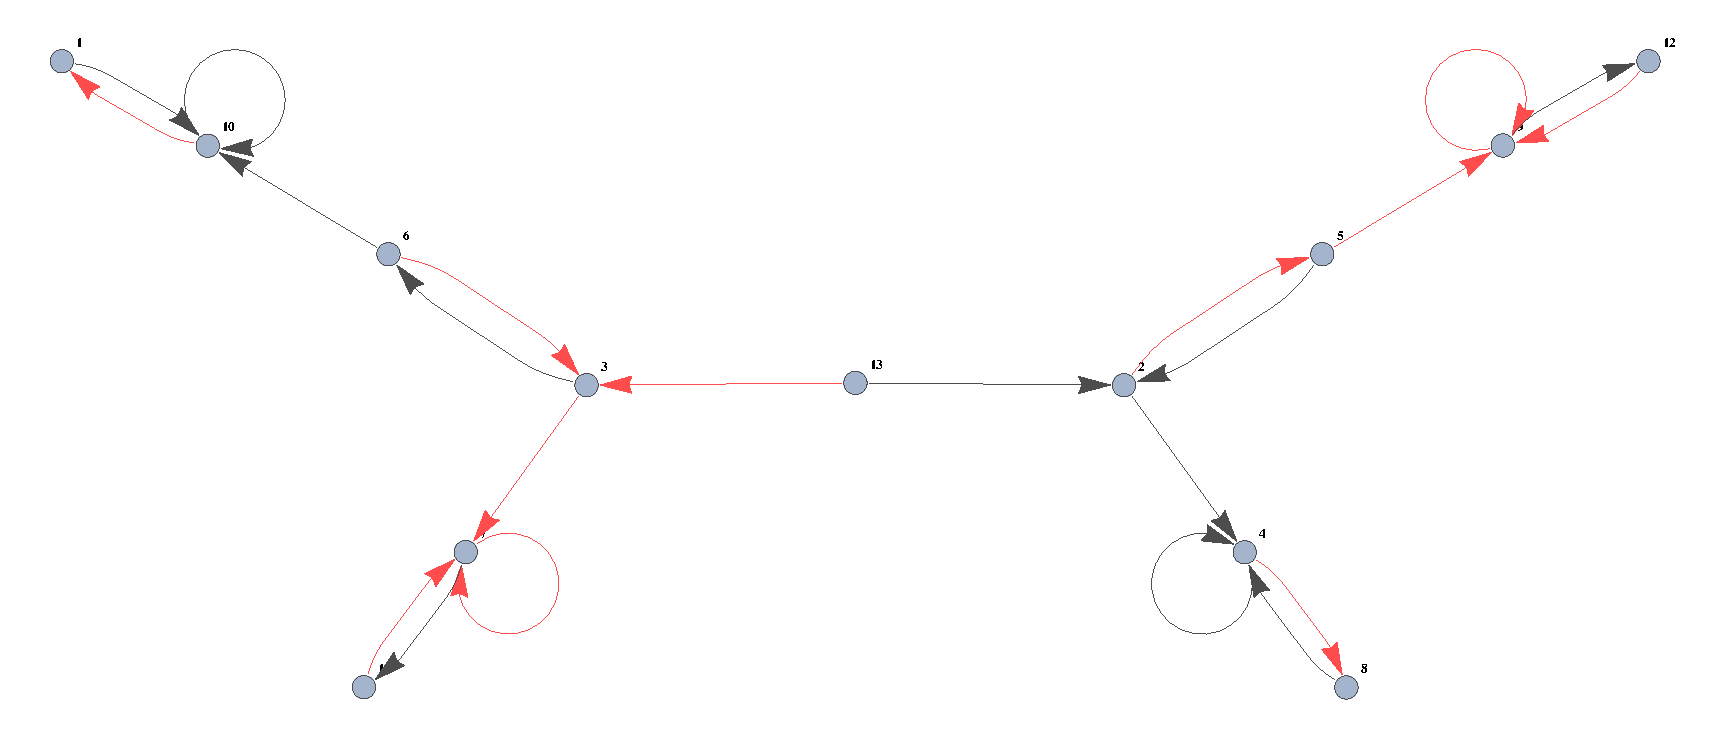
\includegraphics[scale=0.60]{img/limit184w.eps}
\caption{Grafo limite da regra 184.}
\label{fig:limit184w}
\end{center}
\end{figure}

\subsection{Nova tabela de complexidade de regras}\label{sec:table}

Conforme já relatado na Seção \ref{sec:problem}, o encadeamento das
funções NetCAStep, MinNet e TrimNet nos trabalhos anteriores estava
equivocado. Como consequência, a construção da tabela de complexidade
de Wolfram foi refeita. As Tabelas \ref{tbl:Table1}, \ref{tbl:Table2}
e \ref{tbl:Table3} apresentam os novos resultados.

\begin{sidewaystable}
\centering
\includegraphics[scale=0.5]{img/Table1.eps}
\caption{Tabela de complexidade de linguagens regulares (1/3).}
\label{tbl:Table1}
\end{sidewaystable}

\begin{sidewaystable}
\centering
\includegraphics[scale=0.5]{img/Table2.eps}
\caption{Tabela de complexidade de linguagens regulares (2/3).}
\label{tbl:Table2}
\end{sidewaystable}

\begin{sidewaystable}
\centering
\includegraphics[scale=0.5]{img/Table3.eps}
\caption{Tabela de complexidade de linguagens regulares (3/3).}
\label{tbl:Table3}
\end{sidewaystable}

Um ponto importante é que, para algumas regras em que os resultados de
\citecustom{wolfram1994} e \citecustom{trafaniuc2004} coincidiram, houve
divergências neste trabalho. Um exemplo é a regra 18, onde Wolfram e
Trafaniuc obtiveram os mesmos resultados mas este trabalho obteve valores
diferentes, embora Wolfram trabalhou com grafos de processo e Trafaniuc
com AFs.

Outra questão é com relação às regras 32, 128, 136, 160, 168, e 224. Estas têm
o número de estados e arestas do grafo limite apresentados em
\citecustom{wolfram1994} mas não há qualquer registro de como seus grafos
de processo limite foram obtidos. O grafo de processo da regra 128 está
em \citecustom{wolfram1984} e é mostrado na Figura \ref{fig:limit128}, mas
não há qualquer indício de onde os outros grafos vieram.

Baseado no comportamento limite da regra 128, neste trabalho foi desenvolvida
uma técnica manual para inferir o grafo de processo limite das outras regras.
A técnica parte das estruturas imutáveis dos grafos dos
sucessivos passos de tempo, observar a evolução do grafo e deduzir o caso
limite.

Por exemplo, observando os grafos da regra 128 (Figura \ref{fig:r128t}, ele
inicia sempre em um conjuntos de 0s, então uma transição em 1 para um
conjunto de 1s.  Então inicia-se um ciclo de volta ao cojunto de 0s; mas a
distância deste ciclo fica cada vez maior conforme aumenta-se o passo de
tempo. Deduz-se então que esta distância tende a $\infty$ conforme
$t \mapsto \infty$, resultando em um segundo conjunto de 0s visto no grafo
limite.

Seguindo a mesma linha de raciocínio, os grafos de processo limites das
outras regras foram também deduzidos.

\begin{figure}[H]
\begin{center}
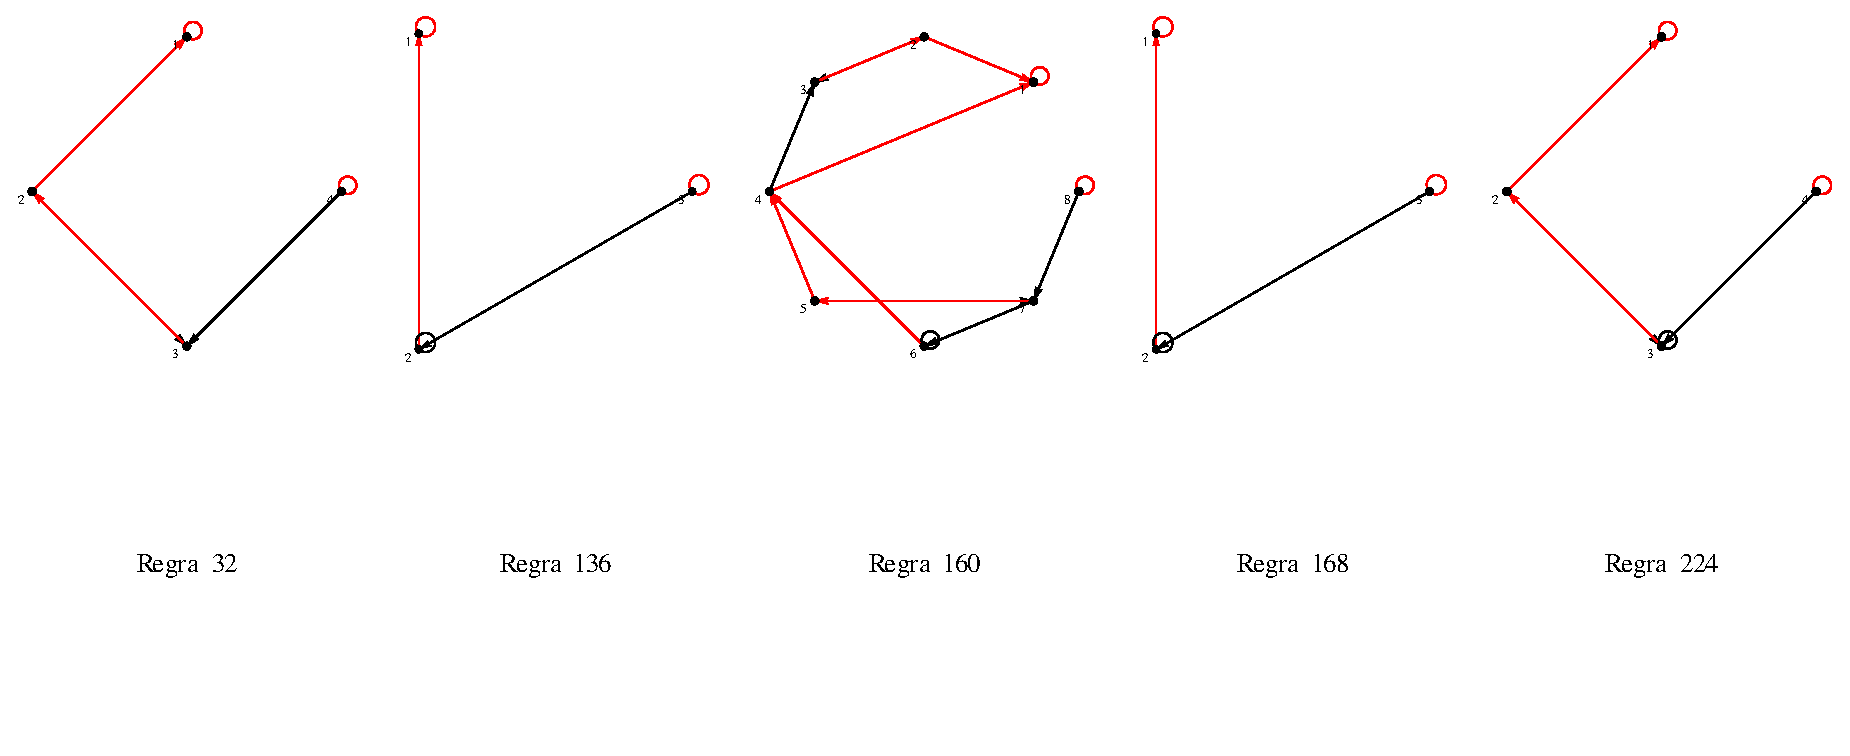
\includegraphics[scale=0.5]{img/Limits.eps}
\caption{Grafos de processo limite.}
\label{fig:limits}
\end{center}
\end{figure}

O mesmo procedimento de validação aplicado ao grafo de processo limite da
regra 184 foi aplicado a estes grafos como forma de evidenciar sua
veracidade.

\newpage

\section{Construção do grafo de processo por meio de matrizes de
adjacências}\label{sec:matrix}

Qualquer grafo pode ter uma representação matricial. Para AFs, é necessário
ainda definir uma forma de representar os estados iniciais e finais. No
caso de grafos de processo, esta informação é irrelevante, pois todos
os estados são iniciais e finais.

\citeonline{wang2011} propuseram uma representação matricial alternativa para
ACs. Eles descreveram a representação linear de sistemas não lineares com
dinâmica local (o que inclui ACs) por meio do produto semi tensorial de
matrizes. A representação linear de tais sistemas é essencialmente uma expansão de
espaço, e qualquer sistema lógico multi agente com $n$ agentes e $m$ estados
pode ser traduzido em um sistema linear de dimensão $m^n$ construindo uma
bijeção adequada. Especificamente, o produto semi tensorial desenvolvido
por \citeonline{cheng2007} fornece uma ferramenta para a construção de
tal bijeção \citecustom{wang2011}.  

Ao final, os autores definem e provam os seguintes teoremas
\citecustom{wang2011}:

\begin{enumerate}
\item Para um sistema linear, todo estado possível do sistema será
atingível a partir de qualquer estado inicial se e somente se os autovalores
da matriz $L_{m^n \times m^n}$ do sistema são
$e^{\frac{2k\pi i}{m^n}},k=0,1,\ldots,m^n-1$, onde $i$ é o número
imaginário tal que $i^2=-1$.

\item Se $e^{\frac{2k\pi i}{r}},k=0,1,\ldots,r-1$ são autovalores de $L$,
então o sistema terá um ciclo de período $r$. Adicionalmente,
o número de séries $\left\{e^{\frac{2k\pi i}{r}}\right\}^{r-1}_{k=0}$
é o número de ciclos de comprimento $r$.

\item O conjunto limite do sistema representado por $L$ consiste de somente um
ponto fixo se e somente se os autovalores da matriz $L$
tem um elemento igual a $1$ e todos os outros iguais a $0$.
\end{enumerate}

Neste capítulo, é proposta uma nova abordagem para o problema, por meio da
análise das matrizes de adjacência correspondentes aos grafos de processo
das respectivas regras do espaço elementar. Porém, como será visto adiante,
não é possível representar completamente um grafo de processo utilizando a
notação clássica de matrizes de adjacência. É proposta, então, uma
nova notação que, dada a matriz de adjacência, é possível construir
integralmente o grafo da respectiva matriz.

O texto então deduz o algoritmo de formação do grafo de processo
de tempo $t$ para a regra 184; e então finaliza com uma breve
descrição dos padrões de formação de matrizes das mesmas regras
estudadas em \citecustom{trafaniuc2004}. O motivo de escolher
a regra 184 para ilustrar o processo se deve ao fato de ser
uma regra que já foi extensivamente estudada em \citecustom{trafaniuc2004}
e \citecustom{miki2006}. No Apêndice \ref{sec:algorithms} os algoritmos
para todas as 26 regras estudadas são apresentados.

\subsection{Representação de grafos de processo em forma matricial}

\subsubsection{Matrizes de adjacências}

Uma \textit{matriz de adjacência}, algumas vezes também chamada de 
\textit{matriz de conexões}, representa os estados e transições de grafos
em forma matricial, rotulando as linhas e colunas com os vértices do grafo.
As linhas e colunas representam, respectivamente, os estados de origem e destino
do grafo\footnote{No caso de grafos não direcionados, não existe
distinção de estados origem e destino, mas somente grafos direcionados são 
de interesse neste trabalho}.

A representação de um grafo direcionado $G$ com $n$ vértices se dá por uma
matriz $M$ de dimensão $n \times n$. O valor da posição $a_{ij}$ da matriz
$M$ será $1$ se existir uma transição do estado $i$ para o estado $j$.
A Figura \ref{fig:graph} mostra um grafo direcionado e a Figura \ref{fig:adjm}
mostra a matriz de adjacência correspondente.

\begin{figure}[ht]
\begin{minipage}[b]{0.5\linewidth}
\begin{center}
\begin{VCPicture}{(0,-4)(4,1)}
\vState[1]{(0,0)}{A} \vState[2]{(4,0)}{B}
\vState[3]{(2,-2)}{C}
\ArcL{A}{B}{} \ArcR{A}{C}{} 
\ArcL{B}{A}{}
\ArcR{C}{B}{} \LoopS{C}{}
\end{VCPicture}
\caption{Grafo direcionado.}
\label{fig:graph}
\end{center}
\end{minipage}
\hspace{0.5cm}
\begin{minipage}[b]{0.5\linewidth}
\begin{center}
\begin{math}
\begin{pmatrix}
0 & 1 & 1 \\
1 & 0 & 0 \\
0 & 1 & 1
\end{pmatrix}
\end{math}
\caption{Representação em matriz de adjacência.}
\label{fig:adjm}
\end{center}
\end{minipage}
\end{figure}

Embora matrizes de adjacência possam representar grafos direcionados simples,
não é possível representar completamente um grafo de processo, dado que:

\begin{enumerate}
\item É possível haver mais de uma transição do estado $i$ para o estado
$j$, $\exists i,j$.

\item Nos índices da matriz não está codificado o valor da transição, que
é o valor esperado na fita de entrada. Observe que a solução de criar
um mapeamento $f: L \mapsto a_{ij}$ que associa o valor do arco ao índice
da matriz é inviável devido à possibilidade de existir mais de uma
transição por par de estados $(i,j)$.
\end{enumerate}

Para ilustrar a dificuldade de se representar grafos de processo utilizando
matrizes de adjacência, considere o grafo de processo da Figura
\ref{fig:initconfigautomaton}. A matriz de adjacência deste autômato
seria uma matriz $1 \times 1$ com valor $a_{1,1}=1$. Porém, perde-se a informação
de que existem duas transições reflexivas no grafo de processo. Mais ainda,
não existe qualquer menção ao valor das transições.

Uma notação possível seria utilizar uma lista em cada índice da matriz de
adjacência. Neste caso, o índice $a_{ij}$ conteria uma lista com todos
os possíveis valores de transição do estado $i$ para o estado $j$.
Porém, com este tipo de notação, além de ser mais complicado
detectar padrões nos sucessivos passos de tempo, perde-se qualquer possibilidade
de operações algébricas com as matrizes. Por exemplo, não seria possível
estudar possíveis padrões baseados nos autovalores das matrizes.

A próxima seção introduz uma notação alternativa de matrizes de
adjacência que contorna as dificuldades apresentadas.

\subsubsection{Matrizes de adjacência de evolução temporal}

Uma matriz de adjacência de evolução temporal é uma notação de matriz de
adjacência para representar grafos de processo que possui uma relação
de isomorfismo entre a matriz e sua representação em grafo.
Formalmente, dado o conjunto de matrizes de adjacência
de evolução temporal $\mathbb{M}$ e o conjunto de grafos de processo $\mathbb{G}$,
existe uma transformação $T: \mathbb{G} \mapsto \mathbb{M}$ e uma
transformação $T^{-1}: \mathbb{M} \mapsto \mathbb{G}$ \citecustom{costa2012}. 

O elemento chave para conseguir essa relação de isomorfismo
é encontrar uma representação do conjunto de transições e
seus respectivos valores em um número real que possa ser codificado
nos índices da matriz, e que possa ser decodificado quando for
aplicada à transformação $T^{-1}$. Formalmente, dado o conjunto de transições
$\mathbb{L}$ do estado $i$ para o estado $j$, $\forall i,j$, encontrar uma
relação $\eta:\mathbb{L} \mapsto \Re$ que seja bijetora.

A resposta para esta questão está em criar um mapeamento dos valores
possíveis de transições para o conjunto de números naturais
$\mathbb{L} \mapsto \mathbb{N}$ e então codificar os valores das transições
em um número binário. Cada bit do número binário corresponde a um valor de
transição. Se o valor no $k$-ésimo bit for 1, significa que existe uma
transição (mapeada no conjunto dos naturais) de valor $k$ do estado de
origem para o estado destino em questão. A operação $\eta$ de codificação dos
arcos $\mathbb{L}$ em um número natural é o polinômio de base 2:

\begin{equation}
\eta(\mathbb{L}_{ij}) = \sum_{\forall k \in (\mathbb{L}_{ij} \mapsto \mathbb{N})} 2^k
\end{equation}

Onde $\mathbb{L}_{ij}$ é o conjunto de transições do estado $i$ para o estado
$j$, o que permite a definição de um espaço de 256 regras possíveis, que são usualmente
identificadas por um número entre 0 e 255 \citecustom{wolfram1984}.
Nota-se que como $k \in \mathbb{N}$, então $\eta(\mathbb{L}_{ij}) \in \mathbb{Z}$,
ou seja, $\eta(\mathbb{L}_{ij})$ está restrita ao domínio dos inteiros. Se
$k \in \mathbb{Z}$ ($\mathbb{L}_{ij} \mapsto \mathbb{Z}$), então
$\eta(\mathbb{L}_{ij}) \in \Re$, pois admitiria-se a possibilidade de expoentes negativos.
Como computacionalmente é mais custoso trabalhar-se com números reais do que com inteiros,
e não há benefício aparente em expandir $\eta$ para o domínio dos reais,
já que $\mathbb{N}$ é contavelmente infinito \citecustom{lewis2008}, optou-se
por restringir-se $\eta$ ao domínio dos números inteiros. Outra observação
é a de que a base númerica não necessariamente deve ser base 2. Poderia-se trabalhar com outras
bases. Todavia, a única implicação na mudança de base é a quantidade de dígitos
necessária para representar um dado conjunto $2^{\mathbb{L}}$ de possíveis combinações de
transições e, do ponto de vista de arquitetura computacional, a base 2 é a
base mais natural para se trabalhar. A Figura \ref{fig:semigraph}
mostra o grafo da Figura \ref{fig:graph}, agora representado como um grafo de processo
(repare que agora existe um valor para cada transição), e a Figura \ref{fig:iadjm}
mostra a matriz de adjacência de evolução temporal correspondente.

\begin{figure}[ht]
\begin{minipage}[b]{0.5\linewidth}
\begin{center}
\begin{VCPicture}{(0,-4)(4,1)}
\vState[1]{(0,0)}{A} \vState[2]{(4,0)}{B}
\vState[3]{(2,-2)}{C}
\ArcL{A}{B}{0} \ArcR{A}{C}{0} 
\ArcL{B}{A}{1}
\ArcR{C}{B}{1} \LoopS{C}{0}
\end{VCPicture}
\caption{Grafo de processo representado através de um grafo direcionado.}
\label{fig:semigraph}
\end{center}
\end{minipage}
\hspace{0.5cm}
\begin{minipage}[b]{0.5\linewidth}
\begin{center}
\begin{math}
\begin{pmatrix}
0 & 1 & 1 \\
2 & 0 & 0 \\
0 & 2 & 1
\end{pmatrix}
\end{math}
\caption{Representação em matriz de adjacência de evolução temporal.}
\label{fig:iadjm}
\end{center}
\end{minipage}
\end{figure}

A transformação de um grafo de processo em uma matriz de adjacência
de evolução temporal é executada por meio do Algoritmo \ref{alg:stom}.

\begin{algorithm}
\caption{Algoritmo para gerar a matriz de adjacência de evolução temporal a partir
de um grafo de processo.}
\label{alg:stom}
\begin{algorithmic}
\STATE $n \leftarrow \mbox{Length}(\mathbb{Q})$ \COMMENT{número de estados}
\STATE $A \leftarrow \psi(n)$
\FORALL{$i,j \in \mathbb{Q}$}
    \IF{$\mathbb{L}_{ij} \neq \emptyset$}
        \STATE $A_{ij} \leftarrow \eta(\mathbb{\mathbb{L}}_{ij})$
    \ENDIF
\ENDFOR
\end{algorithmic}
\end{algorithm}

Onde $\psi(n) = \mbox{ matriz nula } n \times n$.
O algoritmo atua criando uma matriz $A_{n \times n}$, onde $n$ é o número
de estados do grafo de processo, e atribuindo à posição $A_{ij}$ o valor
da função $\eta(\mathbb{L}_{ij}),\forall i,j$, onde $\mathbb{L}_{ij}$
é o conjunto de transições de $i$ para $j$.

O algoritmo de transformação de uma matriz de adjacência de evolução temporal em
um grafo de processo é baseado na representação binária dos valores dos
índices da matriz. Por exemplo, se no índice $A_{1,2}$ existir o valor
$3$, então existe uma transição em $0$ e uma transição em $1$ do estado
\emph{1} para o estado \emph{2}, pois $2^0+2^1=3$. O Algoritmo \ref{alg:mtos}
mostra o processo de geração do grafo de processo a partir de uma matriz de
adjacência de evolução temporal. O algoritmo pressupõe a existência de uma função
\emph{MakeTransition(i,j,m)} que cria uma transição em \emph{m} do estado
\emph{i} para o estado \emph{j}.

\begin{algorithm}
\caption{Algoritmo para gerar o grafo de processo a partir de uma matriz de
adjacência de evolução temporal.}
\label{alg:mtos}
\begin{algorithmic}
\FOR{$i=1$ to $n$}
    \FOR{$j=1$ to $n$}
        \IF{$A_{ij} \neq 0$}
            \REPEAT
                \STATE $q \leftarrow \lfloor A_{ij} \div 2 \rfloor$
                \STATE $r \leftarrow Mod(A_{ij},2)$
                \IF{$r \neq 0$}
                    \STATE $n \leftarrow 0$
                    \WHILE{$2^n \le A_{ij}$}
                        \STATE $n \leftarrow n+1$
                    \ENDWHILE
                    \STATE MakeTransition$(i,j,n-1)$
                \ENDIF
            \UNTIL{$q \neq 0$}
        \ENDIF
    \ENDFOR
\ENDFOR
\end{algorithmic}
\end{algorithm}

O algoritmo executa em tempo $O(n^2)$ em relação à dimensão da matriz.
De posse do Algoritmo \ref{alg:mtos}, é possível criar o algoritmo para gerar o
autômato limite de uma regra apenas elaborando-se um outro algoritmo para gerar a
matriz de adjacência de evolução temporal da regra. A próxima seção apresenta este
algoritmo para a regra 184.

\subsection{Algoritmo do grafo de processo de tempo \emph{t} para a regra 184}\label{sec:184}

Esta seção mostra como utilizar a notação de matriz de adjacência
de evolução temporal para deduzir um algoritmo que gere o grafo de processo de uma
regra do espaço elementar para um passo de tempo discreto $t$ qualquer. Em
particular, aqui é deduzido o algoritmo para gerar a matriz de evolução temporal para
a regra 184 e, a partir desta, poderá ser aplicado o Algoritmo \ref{alg:mtos}
para obtenção do grafo de processo.

\citeonline{miki2006}, baseado nos resultados de \citeonline{trafaniuc2004},
estudou extensivamente o padrão de crescimento da regra 184 através da análise
dos grafos de processo gerados pelos sucessivos passos de tempo. No caso, ele estudou
os grafos de processo gerados dentro dos cinco primeiros passos de tempo. A Figura
\ref{fig:184-5t} mostra os grafos de processo da regra 184 gerados para os cinco
primeiros passos de tempo. A notação de grafo é a mesma da Figura
\ref{fig:initconfigmathematica}.

\begin{figure}[htp]
\begin{center}
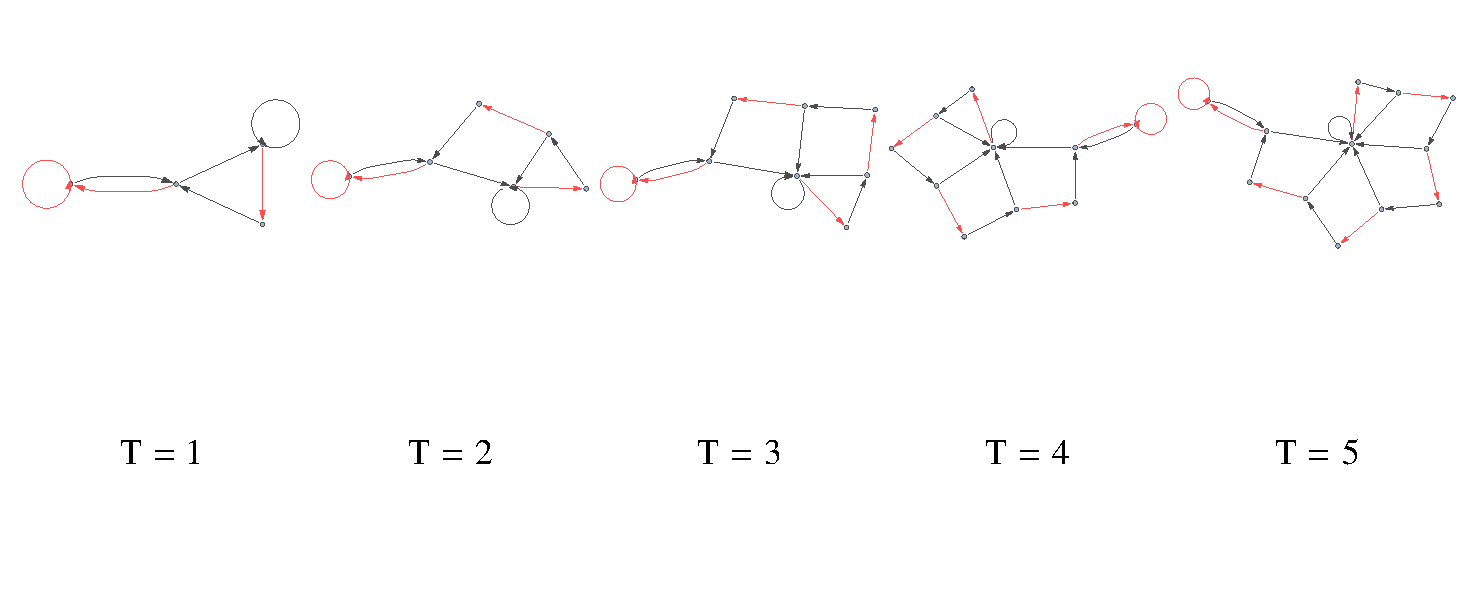
\includegraphics[scale=1]{img/184_5t.eps}
\caption{Grafos de processo para os cinco primeiros passos de tempo da regra 184.}
\label{fig:184-5t}
\end{center}
\end{figure}

Utilizando o método apresentado na Seção \ref{sec:mikialgo}, sua conclusão
foi a de que a cada passo de tempo, sempre existia uma mesma estrutura
de grafo sendo adicionada e uma sendo excluída, e essas estruturas eram
invariantes no tempo. As Figuras \ref{fig:addstruct} e \ref{fig:excstruct}
mostram, respectivamente, as estruturas adicionada e excluída dos sucessivos
grafos de processo da regra 184.

\begin{figure}[htp]
\begin{minipage}[b]{0.5\linewidth}
\centering
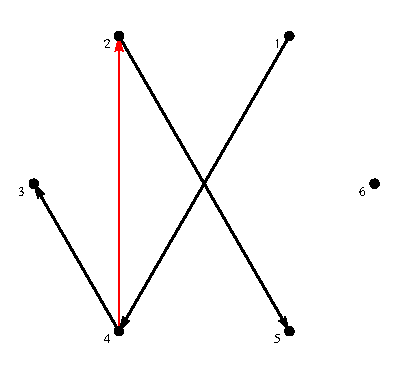
\includegraphics[scale=1]{img/addStruct.eps}
\caption{Estrutura adicionada \citecustom{miki2006}.}
\label{fig:addstruct}
\end{minipage}
\hspace{0.5cm}
\begin{minipage}[b]{0.5\linewidth}
\centering
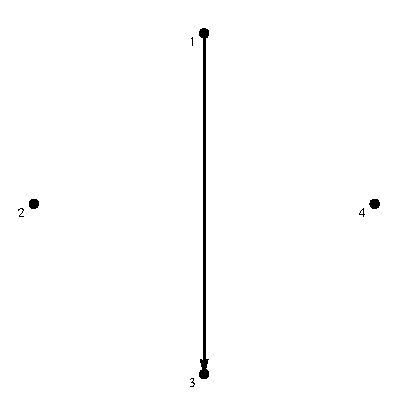
\includegraphics[scale=1]{img/excStruct.eps}
\caption{Estrutura excluída \citecustom{miki2006}.}
\label{fig:excstruct}
\end{minipage}
\end{figure}

É difícil identificar visualmente estas estruturas, ou qualquer padrão de
crescimento, por meio dos grafos de processo. Porém, convertendo estes grafos
em matrizes de adjacência de evolução temporal, é possível detectar os padrões
de crescimento e visualizar o efeito das estruturas adicionada e
excluída. As Figuras \ref{fig:addstructm} e \ref{fig:excstructm} mostram
as respectivas estruturas adicionada e excluída em notação matricial, e
a Tabela \ref{tab:mr184} mostra a evolução no tempo da regra 184 em notação
de grafo e matricial.

\begin{figure}[htp]
\begin{minipage}[b]{0.5\linewidth}
\begin{center}
\begin{math}
\begin{pmatrix}
0 & 0 & 0 & 2 & 0 & 0 \\
0 & 0 & 0 & 0 & 2 & 0 \\
0 & 0 & 0 & 0 & 0 & 0 \\
0 & 1 & 2 & 0 & 0 & 0 \\
0 & 0 & 0 & 0 & 0 & 0 \\
0 & 0 & 0 & 0 & 0 & 0
\end{pmatrix}
\end{math}
\caption{Estrutura adicionada em notação matricial.}
\label{fig:addstructm}
\end{center}
\end{minipage}
\hspace{0.5cm}
\begin{minipage}[b]{0.5\linewidth}
\begin{center}
\begin{math}
\begin{pmatrix}
0 & 0 & 2 & 0 \\
0 & 0 & 0 & 0 \\
0 & 0 & 0 & 0 \\
0 & 0 & 0 & 0
\end{pmatrix}
\end{math}
\caption{Estrutura excluída em notação matricial.}
\label{fig:excstructm}
\end{center}
\end{minipage}
\end{figure}

\begin{table}[H]
\begin{center}
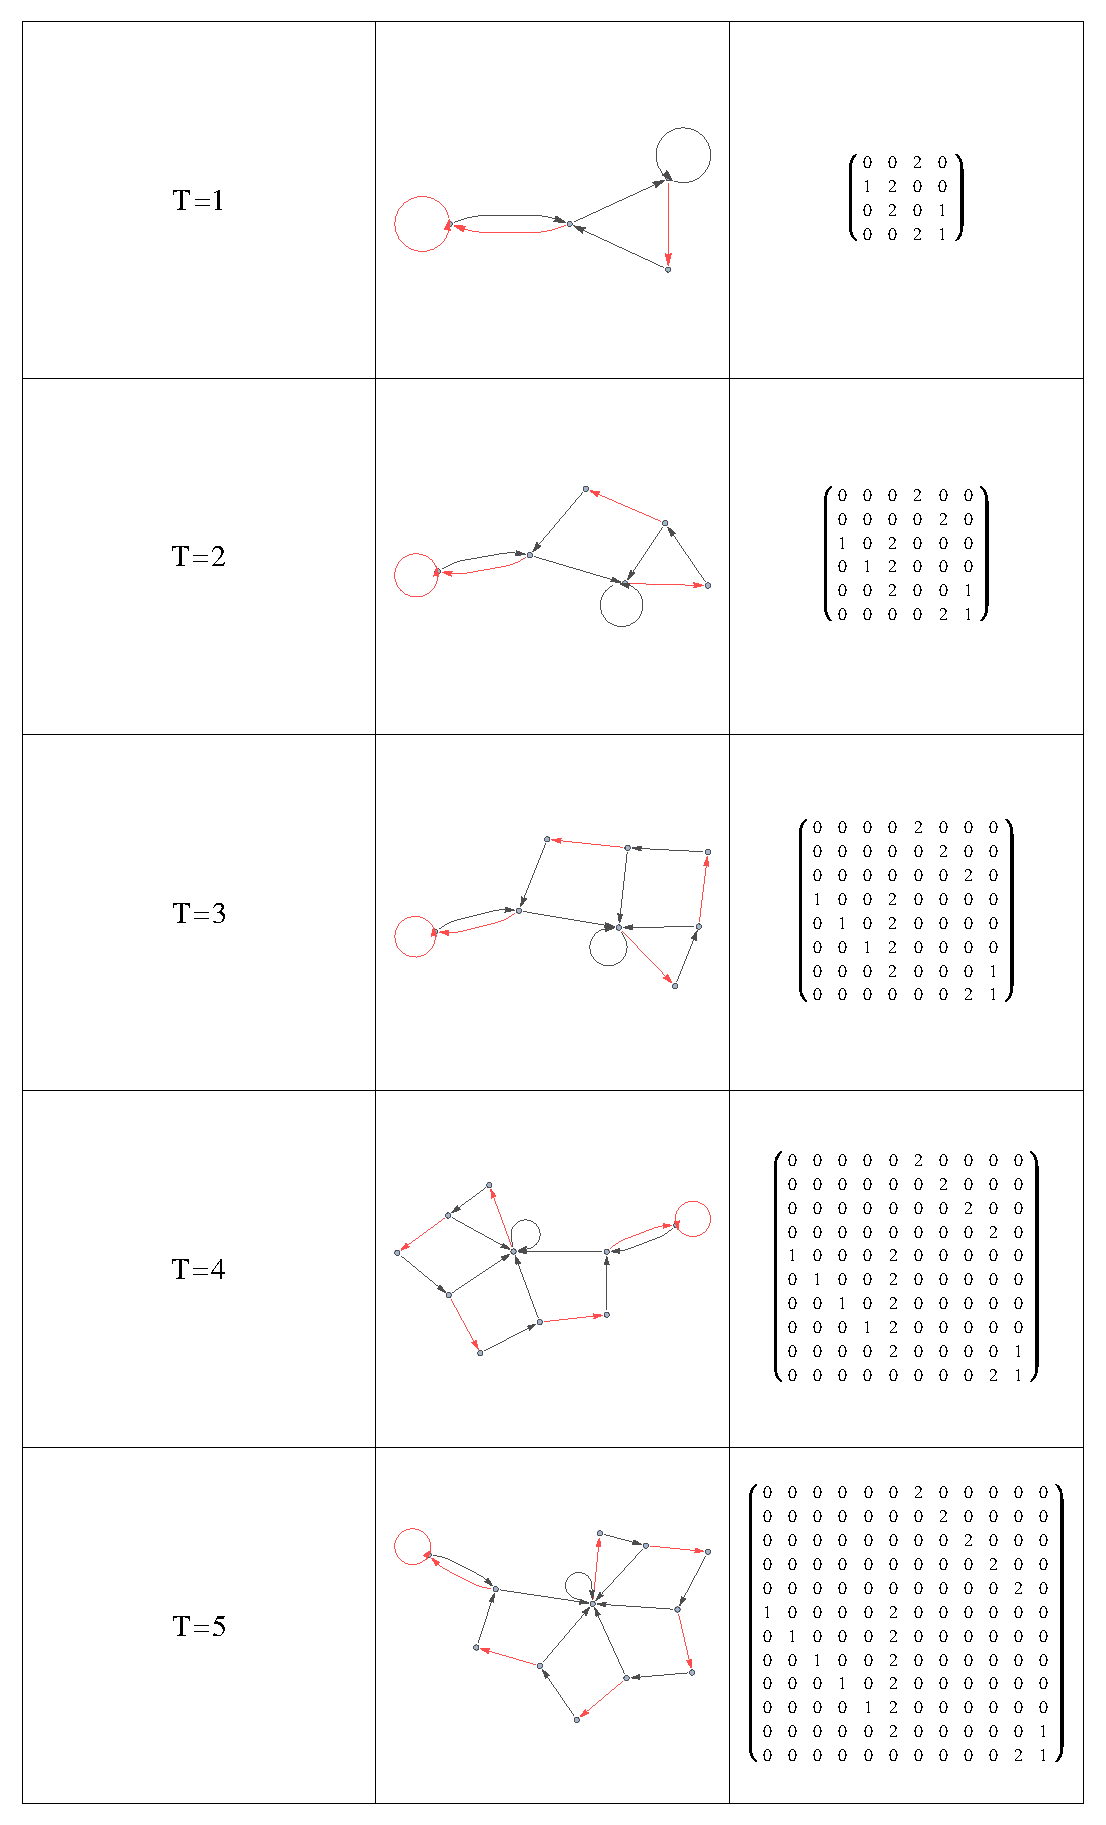
\includegraphics[scale=0.32]{img/mat/matr184.eps}
\caption{Regra 184.}
\label{tab:mr184}
\end{center}
\end{table}

Embora devido à diferença nos tamanhos das matrizes não seja possível
derivar uma operação algébrica, é fácil notar o que acontece na evolução
da regra 184 olhando as matrizes de adjacência da regra e as estruturas
adicionada e excluída.

Observando duas matrizes de tempo $t$ e tempo $t+1$, repara-se que:

\begin{enumerate}
\item Existe uma diagonal de transições em $1$ que começa em $A_{t+1,1}$
e vai até $A_{2t,t}$. A cada passo de tempo, uma transição em $1$ é adicionada,
o que corresponde ao valor $1$ na posição $(4,2)$ da estrutura adicionada.

\item Existe uma coluna de transições em $2$ iniciando-se na posição
$A_{t+1,t+1}$ e terminando na posição $A_{n-1,t+1}$. Novamente observa-se
que a cada passo de tempo, uma linha com uma transição em $2$ é adicionada à
coluna, e essa transição corresponde ao valor $2$ na posição $(4,3)$ na matriz da
estrutura adicionada.

\item Uma diagonal de transições em $2$ aparece na posição $A_{1,t+2}$ indo
até a posição $A_{t,n-1}$. Olhando para a matriz da estrutura adicionada,
observa-se que duas transições em $2$ são adicionadas a esta diagonal a cada
passo de tempo, mas uma dessas transições é retirada conforme se nota na
matriz da estrutura excluída.

\item Por fim, uma transição em $1$ é atribuída à posição $A_{n,n}$, uma
outra transição em $1$ na posição $A_{n-1,n}$ e uma transição em $2$ é
atribuída na posição $A_{n,n-1}$.
\end{enumerate}

Baseando-se nesta análise, é possível derivar um algoritmo de construção da
matriz de adjacência de evolução temporal do grafos de processo de tempo $t$ para a
regra 184. O algoritmo é mostrado no Algoritmo \ref{alg:r184}.

O algoritmo executa em tempo $O(t)$. A combinação dos Algoritmos
\ref{alg:mtos} e \ref{alg:r184} executa em tempo:

\begin{equation}
\begin{tabular}{ r c l }
\(T\) & \(=\) & \(O(t) + O((2t+2)^2)\) \\
  & \(=\) & \(O(t) + O(4t^2+8t+4)\) \\
  & \(=\) & \(O(t) + O(t^2) + O(t) + O(1)\) \\
  & \(=\) & \(O(t^2)\)
\end{tabular}
\end{equation}

De posse do Algoritmo \ref{alg:r184} e do Algoritmo \ref{alg:mtos} é
possível, então, recriar o grafo de processo de tempo $t$ para a regra 184.

\subsection{Padrão de formação das matrizes de adjacências de evolução temporal}\label{sec:pattern}

Após um estudo aprofundado e dedução do algoritmo de formação das matrizes
de adjacência de evolução temporal para a regra 184 descrito na Seção \ref{sec:184},
estudou-se o padrão de formação para todas as mesmas 26 regras estudadas em
\citecustom{trafaniuc2004}. Conforme mostrado na Tabela \ref{tab:pattern},
todas as regras apresentam um padrão de formação, embora nem sempre a
partir do primeiro instante de tempo.

\begin{table}[htp]
\begin{center}
\begin{tabular}{c c c}
\hline
\textbf{Regra} & \textbf{Início do padrão de formação} & \textbf{Linear}\\ \hline
 11 & $t=4$ & Não \\
 14 & $t=4$ & Não \\
 23 & $t=2$ & Sim \\
 35 & $t=3$ & Não \\
 43 & $t=2$ & Sim \\
 50 & $t=3$ & Não \\
 56 & $t=2$ & Sim \\
 70 & $t=3$ & Não \\
 81 & $t=3$ & Não \\
 98 & $t=3$ & Sim \\
113 & $t=2$ & Sim \\
128 & $t=1$ & Sim \\
132 & $t=2$ & Sim \\
136 & $t=2$ & Sim \\
140 & $t=2$ & Sim \\
142 & $t=2$ & Sim \\
162 & $t=2$ & Sim \\
168 & $t=2$ & Sim \\
172 & $t=2$ & Sim \\
176 & $t=2$ & Sim \\
184 & $t=1$ & Sim \\
192 & $t=2$ & Sim \\
196 & $t=1$ & Sim \\
212 & $t=2$ & Sim \\
224 & $t=2$ & Sim \\
232 & $t=2$ & Sim \\
\end{tabular}
\caption{Padrão de formação de matrizes de adjacência de evolução temporal das
regras elementares.}
\label{tab:pattern}
\end{center}
\end{table}

Além de especificar a regra, a tabela mostra em que passo de tempo a regra
começou a apresentar um padrão de formação e se esse padrão é linear
ou não. Por \textit{padrão de formação} entende-se por uma estrutura
presente em $t$ que pode ser vista em $t+1$ de forma expandida ou contraída.
Um \textit{padrão de formação linear} significa que uma
expansão de um padrão na matriz ocorre linearmente com o tempo.

A partir da Tabela \ref{tab:pattern}, conclui-se que as regras estão divididas
em dois grupos base: as que apresentam um padrão linear a partir de $t=n$ e as que
apresentam um padrão não linear a partir de $t=n,\exists n \in \mathbb{N}$.
A análise baseou-se a partir da observação dos cinco primeiros passos de
tempo e, quando o padrão de formação se deu a partir de $t=4$, analisou-se
os dez primeiros passos de tempo.

Com base nesta análise, foram construídos os algoritmos de geração da matriz
de passo de tempo $t$ para a outras 25 regras restantes. Os algoritmos de todas as
26 regras são apresentados no apêndice \ref{sec:algorithms}.

\newpage

\section{Conclusão}\label{sec:conclude}

Autômatos celulares são sistemas totalmente discretos que agem localmente
de forma simples e determinística, mas que podem possuir
comportamento global resultante extremamente complexo. O conjunto de
configurações globais que podem ser vistas em um AC após um determinado
número de passos de evolução pode ser descrito por uma linguagem
regular. Linguagens regulares são aquelas que sempre podem ser reconhecidas
por um autômato finito.

O objetivo deste trabalho é dar continuidade aos trabalhos de
\citeonline{trafaniuc2004} e \citeonline{miki2006}, onde foram feitas
análises dos grafos de processo dos diferentes passos de tempo
para as regras elementares.

Durante a pesquisa, foram encontradas inconsistências nos trabalhos anteriores,
fruto da ambiguidade da descrição das funções NetCAStep, MinNet e TrimNet 
em \citecustom{wolfram2002}. A tabela de \citecustom{wolfram1994} foi novamente
refeita, e novos resultados apareceram, inclusive uma técnica para inferir
o comportamento limite de regras quando isto é possível. O grafo de processo
limite da regra 184 também foi inferido, mas partindo-se da expressão regular
que descreve seu comportamento. Os testes realizados evidenciam que o grafo
de processo apresentado pode ser o grafo limite da regra. A implementação do
algoritmo de seleção de regras de \citecustom{trafaniuc2004} apresenta um
problema com relação a operação de diferença de grafos, e um método para
resolvê-lo ainda não foi obtido.

Outra estratégia foi a de converter os grafos de processo dos sucessivos
passos de tempo das regras do espaço elementar em matrizes de adjacência e analisar
tais matrizes. Porém, a notação comumente utilizada para matrizes de adjacência
não consegue completamente descrever os grafos de processo. É, então, proposta uma
nova notação de matriz de adjacência, chamada de \textit{matriz de
adjacência de evolução temporal}. Com isso, é possível construir o
grafo de processo a partir de sua matriz de adjacência de evolução temporal.

Especificamente, mostrou-se aqui que é possível deduzir um algoritmo para o
grafo de processo de tempo $t$ da regra 184 baseado na análise das respectivas
matrizes de adjacência. Em seguida, analisou-se
os padrões de evolução das matrizes para as 26 regras estudadas em
\citecustom{trafaniuc2004}, evidenciando-se que esse grupo de regras
também apresenta padrão de formação, embora nem sempre desde o primeiro
instante de tempo, da mesma maneira que \citeonline{trafaniuc2004} e
\citeonline{miki2006} já haviam demonstrado para a notação em grafo de processo.
\citeonline{trafaniuc2004} deduziu a regra de formação do autômato de
tempo $t$ para outras 11 regras, além da regra 184. \citeonline{miki2006}
conseguiu automatizar o processo de detecção de padrões em tempos adjacentes
dos grafos de processo que representam a evolução dos ACs, ainda dentro do
conjunto de 26 regras abordadas. Baseando-se nos padrões de formação, foi
deduzido o algoritmo da matriz de evolução temporal para as outras 25 regras.

Acredita-se então que essa nova representação por meio de matrizes de
adjacência possa ajudar no estudo da complexidade de ACs e na identificação
de padrões de crescimento dos respectivos grafos de processo.

Resumidamente, este trabalho apresentou as seguintes críticas aos estudos
anteriores e contribuições:

\begin{itemize}
\item A ordem de chamada das funções NetCAStep, MinNet e TrimNet estava
equivocada nos trabalhos de \citecustom{trafaniuc2004} e \citecustom{miki2006}.
A ordem das funções MinNet e TrimNet estava invertida e o ponto de
realimentação de NetCAStep estava incorreto. A Figura \ref{fig:net} mostra o
encademento correto das funções.

\item O algoritmo de seleção de regras de \citecustom{trafaniuc2004} possui
um problema de implementação na operação de diferença de grafos. Dependendo
de como os vértices são nomeados, diferentes resultados na operação de
diferença ocorrem. Este problema causa a aparição de falsos negativos no
algoritmo.

\item O suposto AF limite da regra 184 apresentado por \citecustom{miki2006}
(Figura \ref{fig:limit184}) não representa o comportamento limite da regra.

\item Devido aos problemas mencionados acima, a tabela de
\citecustom{wolfram1994} foi novamente reconstruída, da mesma forma que
\citecustom{trafaniuc2004} já havia feito.

\item A tabela de \citecustom{wolfram1994} apresentou o número de estados
e transições do grafo de processo limite para algumas regras, mas não
apresentou esses grafos e nem documentou como foram obtidos. Neste trabalho
foi desenvolvida uma técnica para inferir o grafo limite dessas regras.

\item Aqui, por meio de uma abordagem baseada em matrizes, foi possível
obter o algoritmo do grafo de passo de tempo $t$ para todas as 26 regras
obtidas pelo algoritmo de seleção de regras de \citecustom{trafaniuc2004}.
\end{itemize}

Permanece aberta, porém, a questão da convergência da evolução dos grafos
de processo da regra 184 para o seu comportamento limite \citecustom{miki2006}.
Como trabalhos futuros, sugere-se trabalhar em um prova formal da veracidade
do grafo de processo da Figura \ref{fig:limit184w} como o grafo limite da regra
184. Também é necessário encontrar um algoritmo de tempo polinomial que resolva
o problema de diferença de grafos apresentado na Seção \ref{sec:problem}.
Pelo fato de este problema ser muito parecido com o de isomorfismo de grafos,
é aconselhável começar a investigação pela literatura existente sobre tal
problema.

Como sugestão final, a exploração da notação matricial foi feita de forma
superficial neste trabalho.  Pesquisas posteriores podem se aprofundar em
tal tema.

\newpage

\def\refname{Referências bibliográficas}
\bibliography{masterthesis}
\addcontentsline{toc}{section}{Referências bibliográficas} 
\bibliographystyle{abnt-alf}

\appendix
\section{Algoritmos para gerar o grafo de processo de tempo $t$ para as 26 regras
estudadas}\label{sec:algorithms}

\begin{algorithm}[H]
\caption{Algoritmo para gerar a matriz de adjacência de evolução temporal do
grafo de processo de tempo $t$ para a regra 11.}
\label{alg:r11}
\begin{algorithmic}
\STATE $k \leftarrow \lfloor t \div 2 \rfloor$
\STATE $m \leftarrow t-2k$
\IF{$t=1$}
    \STATE $n \leftarrow 3$
    \STATE $A \leftarrow \psi(n)$
    \STATE $A_{n,n-1} \leftarrow 2$
\ELSE
    \STATE $n \leftarrow 2(t+1)$
    \STATE $A \leftarrow \psi(n)$
    \STATE $A_{n-2,n-1} \leftarrow 2$
    \STATE $A_{n,n-2} \leftarrow 2$
    \FOR {$j=1$ to $k$}
        \STATE $A_{k+j,j} \leftarrow 1$
        \STATE $A_{j,t+k+j} \leftarrow 2$
    \ENDFOR
    \FOR {$j=1$ to $k+m$}
        \STATE $A_{t+k+j,k+1} \leftarrow 1$
    \ENDFOR
    \IF {$t > 2$}
        \FOR {$j=1$ to $k+m-1$}
            \STATE $A_{t+k+j,t+j-m} \leftarrow 2$
        \ENDFOR
    \ENDIF
\algstore{rule11}
\end{algorithmic}
\end{algorithm}

\begin{algorithm}[H]
\begin{algorithmic}
\algrestore{rule11}
    \IF {$t>3$}
        \FOR {$j=1$ to $k-1$}
            \STATE $A_{t+j-m,k+j+1} \leftarrow 1$
        \ENDFOR
    \ENDIF
    \IF {$m \ne 0$}
        \STATE $A_{3k,3k+1} \leftarrow 1$
    \ENDIF
\ENDIF
\STATE $A_{n-1,t+k} \leftarrow 1$
\STATE $A_{n,n} \leftarrow 1$
\STATE $A_{n-1,n-1} \leftarrow 2$
\STATE $A_{t+k,n} \leftarrow 1$
\end{algorithmic}
\end{algorithm}

\begin{algorithm}[H]
\caption{Algoritmo para gerar a matriz de adjacência de evolução temporal do
grafo de processo de tempo $t$ para a regra 14.}
\label{alg:r14}
\begin{algorithmic}
\STATE $k \leftarrow \lfloor t \div 2 \rfloor$
\STATE $m \leftarrow t-2k$
\IF{$t=1$}
    \STATE $n \leftarrow 3$
    \STATE $A \leftarrow \psi(n)$
    \STATE $A_{1,n} \leftarrow 1$
    \STATE $A_{2,n} \leftarrow 1$
    \STATE $A_{n,n} \leftarrow 1$
    \STATE $A_{2,1} \leftarrow 2$
    \STATE $A_{n,2} \leftarrow 2$
\ELSE
\algstore{rule14}
\end{algorithmic}
\end{algorithm}

\begin{algorithm}[H]
\begin{algorithmic}
\algrestore{rule14}
    \STATE $n \leftarrow 2(t+1)$
    \STATE $A \leftarrow \psi(n)$
    \FOR{$j=1$ to $k$}
        \STATE $A_{t+k+m+j-1,j} \leftarrow 2$
        \STATE $A_{t+k+m+j-1,t+k+m} \leftarrow 1$
    \ENDFOR
    \IF{$t>2$}
        \FOR{$j=1$ to $k+m-1$}
            \STATE $A_{j,k+j} \leftarrow 2$
            \STATE $A_{k+j,t+j-1} \leftarrow 1$
        \ENDFOR
    \ENDIF
    \IF{$t>3$}
        \FOR{$j=1$ to $k-1$}
            \STATE $A_{t+j-1,t+k+m+j} \leftarrow 1$
        \ENDFOR
    \ENDIF
    \IF{$m=0$}
        \STATE $A_{k,t+k-1} \leftarrow 2$
    \ELSE
        \STATE $A_{3k,n-1} \leftarrow 1$
    \ENDIF
    \STATE $A_{n-2,n} \leftarrow 1$
    \STATE $A_{t+k+m-1,n} \leftarrow 1$
    \STATE $A_{n,n-1} \leftarrow 1$
    \STATE $A_{n,n-2} \leftarrow 2$
    \STATE $A_{n-1,n-2} \leftarrow 2$
    \STATE $A_{n-1,t+k+m} \leftarrow 1$
    \STATE $A_{n-2,t+k+m-1} \leftarrow 2$
\ENDIF
\end{algorithmic}
\end{algorithm}

\begin{algorithm}[H]
\caption{Algoritmo para gerar a matriz de adjacência de evolução temporal do
grafo de processo de tempo $t$ para a regra 23.}
\label{alg:r23}
\begin{algorithmic}
\STATE $n \leftarrow 4t+6$
\STATE $A \leftarrow \psi(n)$
\IF{$t>1$}
    \FOR{$j=1$ to $t-1$}
        \STATE $A_{j,j+1} \leftarrow 2$
        \STATE $A_{t+j,t+j+1} \leftarrow 1$
        \STATE $A_{2t+j,2t+j+2} \leftarrow 2$
        \STATE $A_{3t+j+2,3t+j+3} \leftarrow 1$
    \ENDFOR
\ENDIF
\FOR{$j=1$ to $t$}
    \STATE $A_{3t+j+2,t} \leftarrow 2$
    \STATE $A_{2t+j+1,2t} \leftarrow 1$
\ENDFOR
\STATE $A_{n,n} \leftarrow 1$
\STATE $A_{n-1,n-1} \leftarrow 2$
\STATE $A_{3t+1,n-1} \leftarrow 2$
\STATE $A_{n-1,n-2} \leftarrow 1$
\STATE $A_{n,n-3} \leftarrow 2$
\STATE $A_{n-2,3t+3} \leftarrow 1$
\STATE $A_{3t+2,1} \leftarrow 2$
\STATE $A_{n-2,3t+2} \leftarrow 2$
\STATE $A_{n-3,2t+1} \leftarrow 1$
\STATE $A_{n-3,2t+2} \leftarrow 2$
\STATE $A_{t,2t+2} \leftarrow 2$
\STATE $A_{2t,3t+3} \leftarrow 1$
\STATE $A_{n-4,n} \leftarrow 1$
\STATE $A_{2t+1,t+1} \leftarrow 1$
\STATE $A_{3t+2,2t+1} \leftarrow 1$
\STATE $A_{2t+1,3t+2} \leftarrow 2$
\end{algorithmic}
\end{algorithm}

\begin{algorithm}[H]
\caption{Algoritmo para gerar a matriz de adjacência de evolução temporal do
grafo de processo de tempo $t$ para a regra 35.}
\label{alg:r35}
\begin{algorithmic}
\STATE $k \leftarrow \lfloor t \div 2 \rfloor$
\STATE $m \leftarrow t - 2k$
\STATE $n \leftarrow t+k+3$
\STATE $A \leftarrow \psi(n)$
\IF{$t>2$}
    \FOR{$j=1$ to $k+m-1$}
        \STATE $A_{j,k+j+1} \leftarrow 2$
    \ENDFOR
\ENDIF
\FOR{$j=1$ to $k+m$}
    \STATE $A_{k+j,t+j} \leftarrow 1$
\ENDFOR
\IF{$t>1$}
    \FOR{$j=1$ to $k$}
        \STATE $A_{t+j,j} \leftarrow 1$
    \ENDFOR
\ENDIF
\FOR{$j=1$ to $k+1$}
    \STATE $A_{t+j,k+1} \leftarrow 2$
\ENDFOR
\IF{$m=0$}
    \STATE $A_{k,n-1} \leftarrow 2$
\ENDIF
\STATE $A_{n,n} \leftarrow 1$
\STATE $A_{n,n-1} \leftarrow 2$
\STATE $A_{n-1,n-1} \leftarrow 2$
\STATE $A_{n-1,n-2} \leftarrow 1$
\STATE $A_{n-2,n} \leftarrow 1$
\end{algorithmic}
\end{algorithm}

\begin{algorithm}[H]
\caption{Algoritmo para gerar a matriz de adjacência de evolução temporal do
grafo de processo de tempo $t$ para a regra 43.}
\label{alg:r43}
\begin{algorithmic}
\STATE $n \leftarrow 4(t+1)$
\STATE $A \leftarrow \psi(n)$
\IF{$t>1$}
    \FOR{$j=1$ to $t-1$}
        \STATE $A_{t+j,2t+j+1} \leftarrow 1$
    \ENDFOR
\ENDIF
\FOR{$j=1$ to $t$}
    \STATE $A_{j,n-t-3+j} \leftarrow 2$
    \STATE $A_{3t+j,t+j} \leftarrow 2$
    \STATE $A_{2t+j,j} \leftarrow 1$
    \STATE $A_{2t+j,3t+1} \leftarrow 2$
\ENDFOR
\FOR{$j=1$ to $t+1$}
    \STATE $A_{3t+j,2t+1} \leftarrow 1$
\ENDFOR
\STATE $A_{n,n} \leftarrow 1$
\STATE $A_{n,n-3} \leftarrow 2$
\STATE $A_{n-1,n-1} \leftarrow 2$
\STATE $A_{n-1,n-2} \leftarrow 1$
\STATE $A_{n-2,n} \leftarrow 1$
\STATE $A_{n-3,n-1} \leftarrow 2$
\STATE $A_{2t,n-2} \leftarrow 1$
\STATE $A_{n-2,3t+1} \leftarrow 2$
\end{algorithmic}
\end{algorithm}

\begin{algorithm}[H]
\caption{Algoritmo para gerar a matriz de adjacência de evolução temporal do
grafo de processo de tempo $t$ para a regra 50.}
\label{alg:r50}
\begin{algorithmic}
\STATE $k \leftarrow \lfloor t \div 2 \rfloor$
\STATE $m \leftarrow t - 2k$
\IF{$t=1$}
    \STATE $n \leftarrow 3$
    \STATE $A \leftarrow \psi(n)$
    \STATE $A_{2,1} \leftarrow 2$
    \STATE $A_{n,2} \leftarrow 2$
    \STATE $A_{1,n} \leftarrow 1$
    \STATE $A_{2,n} \leftarrow 1$
    \STATE $A_{n,n} \leftarrow 1$
\ELSE
    \STATE $n \leftarrow 2t+3$
    \STATE $A \leftarrow \psi(n)$
    \FOR{$j=1$ to $k+m-1$}
        \STATE $A_{k+j,j} \leftarrow 1$
        \STATE $A_{t+k+j,2k+j+1} \leftarrow 1$
        \STATE $A_{t+k+j,t} \leftarrow 2$
    \ENDFOR
    \FOR{$j=1$ to $k-1$}
        \STATE $A_{t+j,3k+2m+j} \leftarrow 2$
        \STATE $A_{j,k+j+1} \leftarrow 2$
    \ENDFOR
    \FOR{$j=1$ to $k$}
        \STATE $A_{t+j,k} \leftarrow 1$
    \ENDFOR
    \IF{$t=2$}
        \STATE $A_{n-1,n-2} \leftarrow 2$
        \STATE $A_{1,n-2} \leftarrow 2$
    \ENDIF
\algstore{rule50}
\end{algorithmic}
\end{algorithm}

\begin{algorithm}[H]
\begin{algorithmic}
\algrestore{rule50}
    \IF{$t>2$}
        \STATE $A_{k,t+k+1} \leftarrow 2$
        \STATE $A_{n-1,n-(k+m+2)} \leftarrow 2$
    \ENDIF
    \STATE $A_{n-2,n} \leftarrow 1$
    \STATE $A_{n,n-1} \leftarrow 1$
    \STATE $A_{n,n-2} \leftarrow 2$
    \STATE $A_{n-1,n-3} \leftarrow 1$
    \STATE $A_{n-3,n-3} \leftarrow 1$
    \STATE $A_{t+k,n-2} \leftarrow 2$
    \STATE $A_{t,t+1} \leftarrow 1$
    \STATE $A_{2t,k+1} \leftarrow 2$
    \STATE $A_{2t+1,t} \leftarrow 2$
\ENDIF
\end{algorithmic}
\end{algorithm}

\begin{algorithm}[H]
\caption{Algoritmo para gerar a matriz de adjacência de evolução temporal do
grafo de processo de tempo $t$ para a regra 56.}
\label{alg:r56}
\begin{algorithmic}
\IF{$t=1$}
    \STATE $n \leftarrow 3$
    \STATE $A \leftarrow \psi(n)$
    \STATE $A_{1,n} \leftarrow 1$
    \STATE $A_{2,1} \leftarrow 2$
\ELSE
    \STATE $n \leftarrow 2t$
    \STATE $A \leftarrow \psi(n)$
    \FOR{$j=1$ to $t-1$}
        \STATE $A_{t+j-1,j} \leftarrow 1$
        \STATE $A_{j,t+j} \leftarrow 2$
        \STATE $A_{t+j,t} \leftarrow 2$
    \ENDFOR
\ENDIF
\STATE $A_{n,n} \leftarrow 1$
\STATE $A_{n-1,n} \leftarrow 1$
\STATE $A_{n,n-1} \leftarrow 2$
\end{algorithmic}
\end{algorithm}

\begin{algorithm}[H]
\caption{Algoritmo para gerar a matriz de adjacência de evolução temporal do
grafo de processo de tempo $t$ para a regra 70.}
\label{alg:r70}
\begin{algorithmic}
\IF{$t=1$}
    \STATE $n \leftarrow 3$
\ELSE
    \IF{$t=2$}
        \STATE $n \leftarrow 7$
    \ELSE
        \STATE $n \leftarrow t+6$
    \ENDIF
\ENDIF
\STATE $k \leftarrow \lfloor t \div 2 \rfloor$
\STATE $m \leftarrow t - 2k$
\STATE $A \leftarrow \psi(n)$
\IF{$t=1$}
    \STATE $A_{1,n} \leftarrow 1$
    \STATE $A_{2,n} \leftarrow 1$
    \STATE $A_{n,n} \leftarrow 1$
    \STATE $A_{2,1} \leftarrow 2$
    \STATE $A_{n,2} \leftarrow 2$
\ELSE
    \IF{$t>2$}
        \FOR{$j=1$ to $k+m-1$}
            \STATE $A_{k+j,1-m+j} \leftarrow 1$
        \ENDFOR
        \FOR{$j=1$ to $4$}
            \STATE $A_{t+j+2,t+j-1} \leftarrow 2$
        \ENDFOR
        \STATE $A_{n-3,n} \leftarrow 1$
    \ENDIF
    \FOR{$j=1$ to $k$}
        \STATE $A_{j,k+m+2} \leftarrow 2$
    \ENDFOR
\algstore{rule70}
\end{algorithmic}
\end{algorithm}

\begin{algorithm}[H]
\begin{algorithmic}
\algrestore{rule70}
    \STATE $A_{t,n} \leftarrow 1$
    \STATE $A_{t+2,n} \leftarrow 1$
    \STATE $A_{n,n-1} \leftarrow 1$
    \STATE $A_{n-1,n-2} \leftarrow 1$
    \STATE $A_{n-2,n-2} \leftarrow 1$
    \IF{$t=2$}
        \STATE $A_{n,n-3} \leftarrow 2$
        \STATE $A_{n-1,n-3} \leftarrow 2$
        \STATE $A_{n-2,3} \leftarrow 2$
    \ENDIF
    \STATE $A_{t+1,k+1} \leftarrow 2$
    \STATE $A_{t+2,k+1} \leftarrow 2$
    \STATE $A_{t+1,1} \leftarrow 1$
\ENDIF
\end{algorithmic}
\end{algorithm}

\begin{algorithm}[H]
\caption{Algoritmo para gerar a matriz de adjacência de evolução temporal do
grafo de processo de tempo $t$ para a regra 81.}
\label{alg:r81}
\begin{algorithmic}
\IF{$t=1$}
    \STATE $n \leftarrow 3$
\ELSE
    \IF{$t=2$}
        \STATE $n \leftarrow 7$
    \ELSE
        \STATE $n \leftarrow 2t+2$
    \ENDIF
\ENDIF
\STATE $k \leftarrow \lfloor t \div 2 \rfloor$
\STATE $m \leftarrow t - 2k$
\STATE $A \leftarrow \psi(n)$
\IF{$j>1$}
    \FOR{$j=1$ to $k$}
        \STATE $A_{j,t+j+m} \leftarrow 2$
        \STATE $A_{n-k+j-1,j} \leftarrow 2$
    \ENDFOR
\ENDIF
\FOR{$j=1$ to $k+m$}
    \STATE $A_{k+j,n-k-m+j} \leftarrow 1$
    \STATE $A_{t+j,t+1} \leftarrow 2$
    \STATE $A_{t+j,k+j} \leftarrow 1$
\ENDFOR
\STATE $A_{n,n-k-1} \leftarrow 2$
\IF{$t>2$}
    \STATE $A_{n-k-1,t} \leftarrow 1$
    \STATE $A_{n-k-1,n-k-2} \leftarrow 2$
\ENDIF
\end{algorithmic}
\end{algorithm}

\begin{algorithm}[H]
\caption{Algoritmo para gerar a matriz de adjacência de evolução temporal do
grafo de processo de tempo $t$ para a regra 98.}
\label{alg:r98}
\begin{algorithmic}
\IF{$t=1$}
    \STATE $n \leftarrow 3$
    \STATE $A \leftarrow \psi(n)$
    \STATE $A_{2,1} \leftarrow 2$
    \STATE $A_{1,n} \leftarrow 1$
    \STATE $A_{2,n} \leftarrow 1$
    \STATE $A_{n,n} \leftarrow 1$
    \STATE $A_{n,n-1} \leftarrow 2$
\ELSE
    \STATE $n \leftarrow 2t$
    \STATE $A \leftarrow \psi(n)$
    \FOR{$j=1$ to $t-1$}
        \STATE $A_{t+j-1,j} \leftarrow 2$
        \STATE $A_{t+j-1,t} \leftarrow 1$
    \ENDFOR
    \IF{$t>2$}
        \FOR{$j=1$ to $t-2$}
            \STATE $A_{j,t+j} \leftarrow 1$
        \ENDFOR
    \ENDIF
    \STATE $A_{n-1,n} \leftarrow 1$
    \STATE $A_{t-1,n} \leftarrow 1$
    \STATE $A_{n,n-1} \leftarrow 2$
    \STATE $A_{n,t} \leftarrow 1$
    \STATE $A_{n-1,t-1} \leftarrow 2$
\ENDIF
\end{algorithmic}
\end{algorithm}

\begin{algorithm}[H]
\caption{Algoritmo para gerar a matriz de adjacência de evolução temporal do
grafo de processo de tempo $t$ para a regra 113.}
\label{alg:r113}
\begin{algorithmic}
\STATE $n \leftarrow 4(t+1)$
\STATE $A \leftarrow \psi(n)$
\IF{$t>1$}
    \FOR{$j=1$ to $t-1$}
        \STATE $A_{j,2t+j+1} \leftarrow 2$
    \ENDFOR
\ENDIF
\FOR{$j=1$ to $t$}
    \STATE $A_{3t+j,j} \leftarrow 2$
    \STATE $A_{t+j,3t+j+1} \leftarrow 1$
    \STATE $A_{2t+j,t+j} \leftarrow 1$
    \STATE $A_{2t+2,2t+1} \leftarrow 2$
\ENDFOR
\FOR{$j=1$ to $t+1$}
    \STATE $A_{3t+j,3t+1} \leftarrow 1$
\ENDFOR
\STATE $A_{n-1,n} \leftarrow 2$
\STATE $A_{n-3,n} \leftarrow 2$
\STATE $A_{n,n-1} \leftarrow 1$
\STATE $A_{n-2,n-1} \leftarrow 1$
\STATE $A_{t,n-2} \leftarrow 2$
\STATE $A_{n,n-2} \leftarrow 2$
\STATE $A_{n-1,n-3} \leftarrow 1$
\STATE $A_{n-2,2t+1} \leftarrow 2$
\end{algorithmic}
\end{algorithm}

\begin{algorithm}[H]
\caption{Algoritmo para gerar a matriz de adjacência de evolução temporal do
grafo de processo de tempo $t$ para a regra 128.}
\label{alg:r128}
\begin{algorithmic}
\STATE $n \leftarrow 2(t+1)$
\STATE $A \leftarrow \psi(n)$
\FOR{$j=1$ to $2t-1$}
    \STATE $A_{j,j+1} \leftarrow 1$
\ENDFOR
\STATE $A_{n,n} \leftarrow 1$
\STATE $A_{n,n-1} \leftarrow 2$
\STATE $A_{n-1,n-1} \leftarrow 2$
\STATE $A_{n-2,n} \leftarrow 1$
\STATE $A_{n-1,1} \leftarrow 1$
\end{algorithmic}
\end{algorithm}

\begin{algorithm}[H]
\caption{Algoritmo para gerar a matriz de adjacência de evolução temporal do
grafo de processo de tempo $t$ para a regra 132.}
\label{alg:r132}
\begin{algorithmic}
\STATE $n \leftarrow 2t+3$
\STATE $A \leftarrow \psi(n)$
\IF{$t>1$}
    \FOR{$j=1$ to $t-1$}
        \STATE $A_{j,j+1} \leftarrow 1$
        \STATE $A_{t+j+1,t+j+2} \leftarrow 1$
    \ENDFOR
\ENDIF
\FOR{$j=1$ to $t$}
    \STATE $A_{t+j+1,t} \leftarrow 2$
\ENDFOR
\STATE $A_{n,n} \leftarrow 1$
\STATE $A_{n-2,n} \leftarrow 1$
\STATE $A_{n,n-1} \leftarrow 2$
\STATE $A_{t,t+2} \leftarrow 1$
\STATE $A_{n-1,t+2} \leftarrow 1$
\STATE $A_{n-1,t+1} \leftarrow 2$
\STATE $A_{t+1,t+1} \leftarrow 2$
\STATE $A_{t+1,1} \leftarrow 1$
\end{algorithmic}
\end{algorithm}

\begin{algorithm}[H]
\caption{Algoritmo para gerar a matriz de adjacência de evolução temporal do
grafo de processo de tempo $t$ para a regra 136.}
\label{alg:r136}
\begin{algorithmic}
\STATE $n \leftarrow t+2$
\STATE $A \leftarrow \psi(n)$
\IF{$t>1$}
    \FOR{$j=1$ to $t-1$}
        \STATE $A_{j,j+1} \leftarrow 1$
    \ENDFOR
\ENDIF
\STATE $A_{n,n} \leftarrow 1$
\STATE $A_{n-2,n} \leftarrow 1$
\STATE $A_{n,n-1} \leftarrow 2$
\STATE $A_{n-1,n-1} \leftarrow 2$
\STATE $A_{n-1,1} \leftarrow 1$
\end{algorithmic}
\end{algorithm}

\begin{algorithm}[H]
\caption{Algoritmo para gerar a matriz de adjacência de evolução temporal do
grafo de processo de tempo $t$ para a regra 140.}
\label{alg:r140}
\begin{algorithmic}
\STATE $n \leftarrow t+3$
\STATE $A \leftarrow \psi(n)$
\IF{$t>1$}
    \FOR{$j=1$ to $t-1$}
        \STATE $A_{j,j+1} \leftarrow 1$
    \ENDFOR
\ENDIF
\STATE $A_{n,n} \leftarrow 1$
\STATE $A_{n-1,n} \leftarrow 1$
\STATE $A_{n-3,n} \leftarrow 1$
\STATE $A_{n,n-1} \leftarrow 2$
\STATE $A_{n-1,n-2} \leftarrow 2$
\STATE $A_{n-2,n-2} \leftarrow 2$
\STATE $A_{n-2,1} \leftarrow 1$
\end{algorithmic}
\end{algorithm}

\begin{algorithm}[H]
\caption{Algoritmo para gerar a matriz de adjacência de evolução temporal do
grafo de processo de tempo $t$ para a regra 142.}
\label{alg:r142}
\begin{algorithmic}
\STATE $n \leftarrow 4(t+1)$
\STATE $A \leftarrow \psi(n)$
\IF{$t>1$}
    \FOR{$j=1$ to $t-1$}
        \STATE $A_{j,2t+j+1} \leftarrow 2$
    \ENDFOR
\ENDIF
\FOR{$j=1$ to $t$}
    \STATE $A_{3t+j,j} \leftarrow 2$
    \STATE $A_{2t+j,t+j} \leftarrow 1$
    \STATE $A_{t+j,3t+j+1} \leftarrow 1$
    \STATE $A_{2t+j,2t+1} \leftarrow 2$
\ENDFOR
\FOR{$j=1$ to $t+1$}
    \STATE $A_{3t+j,3t+1} \leftarrow 1$
\ENDFOR
\STATE $A_{n-1,n} \leftarrow 2$
\STATE $A_{n,n-1} \leftarrow 1$
\STATE $A_{n,n-2} \leftarrow 2$
\STATE $A_{n-2,n-1} \leftarrow 1$
\STATE $A_{n-1,n-3} \leftarrow 1$
\STATE $A_{t,n-2} \leftarrow 2$
\STATE $A_{n-2,2t+1} \leftarrow 2$
\STATE $A_{n-3,n} \leftarrow 2$
\end{algorithmic}
\end{algorithm}

\begin{algorithm}[H]
\caption{Algoritmo para gerar a matriz de adjacência de evolução temporal do
grafo de processo de tempo $t$ para a regra 162.}
\label{alg:r162}
\begin{algorithmic}
\STATE $n \leftarrow 2t+3$
\STATE $A \leftarrow \psi(n)$
\FOR{$j=1$ to $t$}
    \STATE $A_{t+j,j} \leftarrow 2$
\ENDFOR
\IF{$t>1$}
    \FOR{$j=1$ to $t-1$}
        \STATE $A_{j,t+j+1} \leftarrow 1$
    \ENDFOR
\ENDIF
\FOR{$j=1$ to $t+2$}
    \STATE $A_{t+j,t+1} \leftarrow 1$
\ENDFOR
\STATE $A_{n-1,n} \leftarrow 2$
\STATE $A_{t,n-1} \leftarrow 1$
\STATE $A_{n,n-1} \leftarrow 1$
\STATE $A_{n,n-2} \leftarrow 2$
\STATE $A_{n-2,n-2} \leftarrow 2$
\end{algorithmic}
\end{algorithm}

\begin{algorithm}[H]
\caption{Algoritmo para gerar a matriz de adjacência de evolução temporal do
grafo de processo de tempo $t$ para a regra 168.}
\label{alg:r168}
\begin{algorithmic}
\STATE $n \leftarrow t+3$
\STATE $A \leftarrow \psi(n)$
\IF{$t>1$}
    \FOR{$j=1$ to $t-1$}
        \STATE $A_{j,j+1} \leftarrow 1$
    \ENDFOR
\ENDIF
\STATE $A_{n,n} \leftarrow 1$
\STATE $A_{n-3,n} \leftarrow 1$
\STATE $A_{n,n-1} \leftarrow 2$
\STATE $A_{n-1,n-1} \leftarrow 2$
\STATE $A_{n-2,n-1} \leftarrow 2$
\STATE $A_{n-1,n-2} \leftarrow 1$
\STATE $A_{n-2,1} \leftarrow 1$
\end{algorithmic}
\end{algorithm}

\begin{algorithm}[H]
\caption{Algoritmo para gerar a matriz de adjacência de evolução temporal do
grafo de processo de tempo $t$ para a regra 172.}
\label{alg:r172}
\begin{algorithmic}
\IF{$t=1$}
    \STATE $n \leftarrow 8$
    \STATE $A \leftarrow \psi(n)$
    \STATE $A_{4,n} \leftarrow 1$
    \STATE $A_{n-1,n-1} \leftarrow 2$
    \STATE $A_{n,n-2} \leftarrow 2$
    \STATE $A_{1,n-2} \leftarrow 2$
    \STATE $A_{n-3,n-2} \leftarrow 2$
    \STATE $A_{n-2,n-3} \leftarrow 2$
    \STATE $A_{5,3} \leftarrow 1$
    \STATE $A_{n-1,4} \leftarrow 1$
    \STATE $A_{n-2,4} \leftarrow 1$
\algstore{rule172}
\end{algorithmic}
\end{algorithm}

\begin{algorithm}[H]
\begin{algorithmic}
\algrestore{rule172}
\ELSE
    \STATE $n \leftarrow t+9$
    \STATE $A \leftarrow \psi(n)$
    \FOR{$j=1$ to $t-1$}
        \STATE $A_{j+1,j+2} \leftarrow 1$
    \ENDFOR
    \STATE $A_{n,n-1} \leftarrow 2$
    \STATE $A_{n-1,n-2} \leftarrow 2$
    \STATE $A_{n-2,n-2} \leftarrow 2$
    \STATE $A_{1,n-3} \leftarrow 2$
    \STATE $A_{n-4,n-3} \leftarrow 2$
    \STATE $A_{n-3,n-4} \leftarrow 2$
    \STATE $A_{t+4,1} \leftarrow 2$
    \STATE $A_{t+3,3} \leftarrow 1$
    \STATE $A_{t+5,t+2} \leftarrow 1$
    \STATE $A_{n-2,t+3} \leftarrow 1$
    \STATE $A_{n-5,n} \leftarrow 1$
    \STATE $A_{n-1,n-5} \leftarrow 1$
    \STATE $A_{n-3,t+3} \leftarrow 1$
\ENDIF
\STATE $A_{n,n} \leftarrow 1$
\STATE $A_{t+1,n} \leftarrow 1$
\STATE $A_{t+2,1} \leftarrow 2$
\STATE $A_{t+3,1} \leftarrow 2$
\STATE $A_{t+2,2} \leftarrow 1$
\end{algorithmic}
\end{algorithm}

\begin{algorithm}[H]
\caption{Algoritmo para gerar a matriz de adjacência de evolução temporal do
grafo de processo de tempo $t$ para a regra 176.}
\label{alg:r176}
\begin{algorithmic}
\STATE $n \leftarrow 2t+3$
\STATE $A \leftarrow \psi(n)$
\FOR{$j=1$ to $t$}
    \STATE $A_{j,t+j} \leftarrow 2$
\ENDFOR
\FOR{$j=1$ to $t-1$}
    \STATE $A_{t+j,j+1} \leftarrow 1$
\ENDFOR
\STATE $A_{n,n} \leftarrow 1$
\STATE $A_{n-1,n} \leftarrow 1$
\STATE $A_{n-3,n} \leftarrow 1$
\STATE $A_{n,n-1} \leftarrow 2$
\STATE $A_{n-1,n-2} \leftarrow 2$
\STATE $A_{n-2,n-2} \leftarrow 2$
\STATE $A_{n-2,1} \leftarrow 1$
\end{algorithmic}
\end{algorithm}

\begin{algorithm}[H]
\caption{Algoritmo para gerar a matriz de adjacência de evolução temporal do
grafo de processo de tempo $t$ para a regra 184.}
\label{alg:r184}
\begin{algorithmic}
\STATE $n \leftarrow 2(t+1)$
\STATE $A \leftarrow \psi(n)$
\STATE $i \leftarrow t+1$
\FOR{$j=1$ to t}
    \STATE $A_{ij} \leftarrow 1$
    \STATE $i \leftarrow i+1$
\ENDFOR
\FOR{$i=t+1$ to $n$}
    \STATE $A_{i,t+1} \leftarrow 2$
\ENDFOR
\STATE $j \leftarrow t+2$
\FOR{$i=1$ to $t$}
    \STATE $A_{ij} \leftarrow 2$
    \STATE $j \leftarrow j+1$
\ENDFOR
\STATE $A_{n,n} \leftarrow 1$
\STATE $A_{n-1,n} \leftarrow 1$
\STATE $A_{n,n-1} \leftarrow 2$
\end{algorithmic}
\end{algorithm}

\begin{algorithm}[H]
\caption{Algoritmo para gerar a matriz de adjacência de evolução temporal do
grafo de processo de tempo $t$ para a regra 192.}
\label{alg:r192}
\begin{algorithmic}
\STATE $n \leftarrow t+2$
\STATE $A \leftarrow \psi(n)$
\FOR{$j=1$ to $t-1$}
    \STATE $A_{j,j+1} \leftarrow 1$
\ENDFOR
\STATE $A_{n,n} \leftarrow 1$
\STATE $A_{n-2,n} \leftarrow 1$
\STATE $A_{n,n-1} \leftarrow 2$
\STATE $A_{n-1,n-1} \leftarrow 2$
\STATE $A_{n-1,1} \leftarrow 1$
\end{algorithmic}
\end{algorithm}

\begin{algorithm}[H]
\caption{Algoritmo para gerar a matriz de adjacência de evolução temporal do
grafo de processo de tempo $t$ para a regra 196.}
\label{alg:r196}
\begin{algorithmic}
\STATE $n \leftarrow t+3$
\STATE $A \leftarrow \psi(n)$
\FOR{$j=1$ to $t$}
    \STATE $A_{j,j+1} \leftarrow 1$
    \STATE $A_{j+1,1} \leftarrow 2$
\ENDFOR
\STATE $A_{n,n} \leftarrow 1$
\STATE $A_{n-2,n} \leftarrow 1$
\STATE $A_{n,n-1} \leftarrow 2$
\STATE $A_{n-1,n-1} \leftarrow 2$
\STATE $A_{n-1,2} \leftarrow 1$
\end{algorithmic}
\end{algorithm}

\begin{algorithm}[H]
\caption{Algoritmo para gerar a matriz de adjacência de evolução temporal do
grafo de processo de tempo $t$ para a regra 212.}
\label{alg:r212}
\begin{algorithmic}
\STATE $n \leftarrow 4(t+1)$
\STATE $A \leftarrow \psi(n)$
\FOR{$j=1$ to $t$}
    \STATE $A_{j,3t+j+1} \leftarrow 2$
    \STATE $A_{3t+j,t+j} \leftarrow 2$
    \STATE $A_{2t+j,j} \leftarrow 1$
    \STATE $A_{2t+j,3t+1} \leftarrow 2$
\ENDFOR
\IF{$t>1$}
    \FOR{$j=1$ to $t-1$}
        \STATE $A_{t+j,2t+j+1} \leftarrow 1$
    \ENDFOR
\ENDIF
\FOR{$j=1$ to $t+1$}
    \STATE $A_{n-(t-j+4),2t+1} \leftarrow 1$
\ENDFOR
\STATE $A_{n,n} \leftarrow 1$
\STATE $A_{n-2,n} \leftarrow 1$
\STATE $A_{n-1,n-1} \leftarrow 2$
\STATE $A_{n-3,n-1} \leftarrow 2$
\STATE $A_{n-1,n-2} \leftarrow 1$
\STATE $A_{n,n-3} \leftarrow 2$
\STATE $A_{n-2,3t+1} \leftarrow 2$
\STATE $A_{2t,n-2} \leftarrow 1$
\end{algorithmic}
\end{algorithm}

\begin{algorithm}[H]
\caption{Algoritmo para gerar a matriz de adjacência de evolução temporal do
grafo de processo de tempo $t$ para a regra 224.}
\label{alg:r224}
\begin{algorithmic}
\STATE $n \leftarrow t+3$
\STATE $A \leftarrow \psi(n)$
\FOR{$j=1$ to $t-1$}
    \STATE $A_{j,j+1} \leftarrow 1$
\ENDFOR
\STATE $A_{n,n} \leftarrow 1$
\STATE $A_{n-3,n} \leftarrow 1$
\STATE $A_{n,n-1} \leftarrow 2$
\STATE $A_{n-1,n-1} \leftarrow 2$
\STATE $A_{n-2,n-1} \leftarrow 2$
\STATE $A_{n-1,n-2} \leftarrow 1$
\STATE $A_{t+1,1} \leftarrow 1$
\end{algorithmic}
\end{algorithm}

%\begin{algorithm}[H]
%\caption{Algoritmo para gerar a matriz de adjacência de evolução temporal do
%grafo de processo de tempo $t$ para a regra 252.}
%\label{alg:r252}
%\begin{algorithmic}
%\STATE $n \leftarrow t+2$
%\STATE $A \leftarrow \psi(n)$
%\FOR{$j=1$ to $t-1$}
%    \STATE $A_{j,j+1} \leftarrow 2$
%\ENDFOR
%\STATE $A_{n,n} \leftarrow 2$
%\STATE $A_{n-2,n} \leftarrow 2$
%\STATE $A_{n,n-1} \leftarrow 1$
%\STATE $A_{n-1,n-1} \leftarrow 1$
%\STATE $A_{n-1,1} \leftarrow 2$
%\end{algorithmic}
%\end{algorithm}

\begin{algorithm}[H]
\caption{Algoritmo para gerar a matriz de adjacência de evolução temporal do
grafo de processo de tempo $t$ para a regra 232.}
\label{alg:r232}
\begin{algorithmic}
\STATE $n \leftarrow 4t+6$
\STATE $A \leftarrow \psi(n)$
\IF{$t>1$}
    \FOR{$j=1$ to $t-1$}
        \STATE $A_{j,j+1} \leftarrow 2$
        \STATE $A_{2t+j+1,2t+j+2} \leftarrow 2$
        \STATE $A_{t+j,t+j+1} \leftarrow 1$
        \STATE $A_{3t+j+2,3t+j+3} \leftarrow 1$
    \ENDFOR
\ENDIF
\FOR{$j=1$ to $t$}
    \STATE $A_{3t+j+2,t} \leftarrow 2$
    \STATE $A_{2t+j+1,2t} \leftarrow 1$
\ENDFOR
\STATE $A_{n,n} \leftarrow 1$
\STATE $A_{n-4,n} \leftarrow 1$
\STATE $A_{3t+1,n-1} \leftarrow 2$
\STATE $A_{n-1,n-1} \leftarrow 2$
\STATE $A_{n-1,n-2} \leftarrow 1$
\STATE $A_{n,n-3} \leftarrow 2$
\STATE $A_{2t,3t+3} \leftarrow 1$
\STATE $A_{n-2,3t+3} \leftarrow 1$
\STATE $A_{n-2,3t+2} \leftarrow 2$
\STATE $A_{2t+1,3t+2} \leftarrow 2$
\STATE $A_{t,2t+2} \leftarrow 2$
\STATE $A_{n-3,2t+2} \leftarrow 2$
\STATE $A_{n-3,2t+1} \leftarrow 1$
\STATE $A_{3t+2,2t+1} \leftarrow 1$
\STATE $A_{3t+2,1} \leftarrow 2$
\STATE $A_{2t+1,t+1} \leftarrow 1$
\end{algorithmic}
\end{algorithm}

\newpage

\end{document}

% vim:set spell spelllang=pt
